\section{Physic Object Recostruction}

\subsection{Primary Vertices object definition}

\begin{table}[htb]
	\caption{definition of Vertex.}
	\label{table:vertexobjdefinition}
	\ttfamily\scriptsize\selectfont
	\begin{center}
		\begin{tabular}{|l|ll|}
			\hline
			\multicolumn{3}{|l|}{collection \texttt{label: recoVertex}}\\
			\multicolumn{3}{|l|}{type: \texttt{offlinePrimaryVertices}}\\
			\hline
			vertex.size() & $>$ & 0 \\
			\hline
		\end{tabular}
	\end{center}
\end{table}

\subsection{Trigger Paths definition}

\begin{table}[htb]
	
	\caption{Trigger paths list.}
	\label{table:triggerdefinition}
	\ttfamily\scriptsize\selectfont
	\begin{center}
		\begin{tabular}{|l|l|}
			\hline
			\multicolumn{2}{|l|}{collection \texttt{label: TriggerResults\_HLT}}\\
			\multicolumn{2}{|l|}{type: \texttt{edm::TriggerResults}}\\
			\hline
			\texttt{HLT\_DoubleMediumIsoPFTau35\_Trk5\_eta2p1\_Prong1\_v2} & OR \\
			\texttt{HLT\_DoubleMediumIsoPFTau35\_Trk5\_eta2p1\_Prong1\_v3} & OR \\
			\texttt{HLT\_DoubleMediumIsoPFTau35\_Trk5\_eta2p1\_Prong1\_v4} & OR \\
			\texttt{HLT\_DoubleMediumIsoPFTau35\_Trk5\_eta2p1\_Prong1\_v6} & OR \\
			\texttt{HLT\_DoubleMediumIsoPFTau35\_Trk1\_eta2p1\_Prong1\_v1} & OR \\
			\texttt{HLT\_DoubleMediumIsoPFTau35\_Trk1\_eta2p1\_Prong1\_v3} & OR \\
			\texttt{HLT\_DoubleMediumIsoPFTau35\_Trk1\_eta2p1\_Prong1\_v4} & \\
			\hline
		\end{tabular}
	\end{center}
\end{table}

\clearpage

\subsection{Jet object definition}

\begin{table}[htb]
  \caption{definition of jets.}
   \label{table:jetobjdefinition}
  \begin{center}
    \ttfamily\scriptsize\selectfont
    \begin{tabular}{|l|ll|}
      \hline
      \multicolumn{3}{|l|}{ collection label: selectedPatJets}\\
      \multicolumn{3}{|l|}{ type: \texttt{pat::Jet}}\\
      \hline
      jet.pt() & $>=$ & 30. \\
      fabs(jet.eta()) & $<=$ & 5.0 \\
      jet.neutralHadronEnergyFraction() & $<$ &  0.99 \\
      jet.neutralEmEnergyFraction() & $<$ & 0.99 \\
      jet.numberOfDaughters() & $>$& 1 \\
      if(fabs(jet.eta()) $<$ 2.4) && \\
      ~~~jet.chargedHadronEnergyFraction() & $>$ & 0 \\
      ~~~jet.chargedEmEnergyFraction() & $<$ & 0.99 \\
      ~~~jet.chargedMultiplicity() & $>$ & 0 \\
      DeltaR(jet,tau) & $>=$ & 0.3 \\
      \hline
    \end{tabular}
  \end{center}
\end{table}

\subsection{b-Jet object definition}

\begin{table}[htb]
  \caption{definition of $b$-jets.}
  \label{table:bjetobjdefinition}
  \begin{center}
  \ttfamily\scriptsize\selectfont
  \begin{tabular}{|l|ll|}
    \hline
    \multicolumn{3}{|l|}{ collection label: selectedPatJets}\\
    \multicolumn{3}{|l|}{ type: \texttt{pat::Jet}}\\
    \hline
    jet.pt() & $>=$ &  30. \\
    fabs(jet.eta()) & $<=$ & 2.4 \\
    DeltaR(jet,tau) & $>=$ & 0.3 \\
    jet.bDiscriminator(?) & $>$ & 0.244 \\
    \hline
  \end{tabular}
  \end{center}
\end{table}

\subsection{Tau object definition}

\begin{table}[htb]
  \caption{definition of \ensuremath{\tau} leptons.}
  \label{table:tauobjdefinition}
  \begin{center}
  \ttfamily\scriptsize\selectfont
  \begin{tabular}{|l|ll|}
    \hline
    \multicolumn{3}{|l|}{ collection label: \texttt{patTaus}}\\
    \multicolumn{3}{|l|}{ type: \texttt{pat::Tau}}\\
    \hline
    fabs(tau.eta()) & $<=$ & 2.1 \\
    tau.pt() & $>=$ & 45.0 \\
    tau.leadPFChargedHadrCand()-$>$pt() & $>=$ & 5.0 \\
    tau.tauID(``byTightIsolationMVA3newDMwLT'') & $>$ & 0.5 ||\\
    ~tau.tauID(``byMediumIsolationMVA3newDMwLT'') & $>$ & 0.5 ||\\
    ~tau.tauID(``byLooseIsolationMVA3newDMwLT'') & $>$ & 0.5 \\
    (decayModeFindingNewDMs & $>$ & 0.5 $\&\&$ \\ 
    ~signalPFChargedHadrCands().size() & $==$ & 1) \\
    tau.tauID(``againstElectronMediumMVA5'') & $>$ & 0.5 \\
    tau.tauID(``againstMuonLoose3'') & $>$ & 0.5 \\
    \hline
  \end{tabular}
  \end{center}
\end{table}

\clearpage

\subsection{MET object definition}

\begin{table}[htb]
  \caption{definition of \met}
  \label{table:metobjdefinition}
  \ttfamily\scriptsize\selectfont
  \begin{center}
   \begin{tabular}{|l|ll|}
      \hline
      \multicolumn{3}{|l|}{ collection \texttt{label: patMET}}\\
      \multicolumn{3}{|l|}{ type: \texttt{patPfMetT0pcT1Txy}}\\
      \hline
    \end{tabular}
  \end{center}
\end{table}

\section{Physic Object Recostruction at 13 TeV}

\subsection{Tau object definition}

\begin{table}[htb]
	\caption{definition of \ensuremath{\tau} leptons.}
	\label{table:tauobjdefinition_13TeV}
	\begin{center}
		\ttfamily\scriptsize\selectfont
		\begin{tabular}{|l|ll|}
			\hline
			\multicolumn{3}{|l|}{ collection label: \texttt{patTaus}}\\
			\multicolumn{3}{|l|}{ type: \texttt{pat::Tau}}\\
			\hline
			fabs(tau.eta()) & $<=$ & 2.1 \\
			tau.pt() & $>=$ & 20 \\
			tau.leadPFChargedHadrCand()-$>$pt() & $>=$ & 5.0 \\
			tau.tauID(``byTightIsolationMVArun2v1DBdR03oldDMwLT'') & $>$ & 0.5 ||\\
			~tau.tauID(``byMediumIsolationMVArun2v1DBdR03oldDMwLT'') & $>$ & 0.5 ||\\
			~tau.tauID(``byLooseIsolationMVArun2v1DBdR03oldDMwLT'') & $>$ & 0.5 \\
			(byLooseIsolationMVArun2v1DBnewDMwLT & $>$ & 0.5 $\&\&$ \\ 
			~signalPFChargedHadrCands().size() & $<$ & 4) \\
			tau.tauID(``againstElectronMediumMVA6'') & $>$ & 0.5 \\
			tau.tauID(``againstMuonLoose3'') & $>$ & 0.5 \\
			\hline
		\end{tabular}
	\end{center}
\end{table}

\subsection{Jet object definition}

\begin{table}[htb]
	\caption{definition of jets.}
	\label{table:jetobjdefinition_13TeV}
	\begin{center}
		\ttfamily\scriptsize\selectfont
		\begin{tabular}{|l|ll|}
			\hline
			\multicolumn{3}{|l|}{ collection label: selectedPatJets}\\
			\multicolumn{3}{|l|}{ type: \texttt{pat::Jet}}\\
			\hline
			jet.pt() & $>=$ & 30. \\
			fabs(jet.eta()) & $<=$ & 5.0 \\
			jet.neutralHadronEnergyFraction() & $<$ &  0.99 \\
			jet.neutralEmEnergyFraction() & $<$ & 0.99 \\
			jet.numberOfDaughters() & $>$& 1 \\
			if(fabs(jet.eta()) $<$ 2.4) && \\
			~~~jet.chargedHadronEnergyFraction() & $>$ & 0 \\
			~~~jet.chargedEmEnergyFraction() & $<$ & 0.99 \\
			~~~jet.chargedMultiplicity() & $>$ & 0 \\
			DeltaR(jet,tau) & $>=$ & 0.3 \\
			\hline
		\end{tabular}
	\end{center}
\end{table}

\section{Monte Carlo Samples at 8 TeV}

\begin{table}[ht]
	\tiny
	\centering{
		\begin{tabular}{| l | l |}
			\hline
			&\\
			Process &Official CMS Datasets /DY*/AODSIM \\
			&\\
			\hline		
			&\\
			$Z \longrightarrow \tau\tau$ & \texttt{ToTauTau\_M-20\_CT10\_TuneZ2star\_v2\_8TeV-powheg-tauola-pythia6/Summer12 DR53X-PU\_S10\_START53\_V7A-v2} \\
			&\\
			$Z \longrightarrow \mu\mu$ & \texttt{ToMuMu\_M-20\_CT10\_TuneZ2star\_v2\_8TeV-powheg-pythia6/Summer12\_DR53X-PU\_S10\_START53\_V7A-v1} \\
			&\\
			$Z \longrightarrow ee$ & \texttt{ToEE\_M-20\_CT10\_TuneZ2star\_v2 8TeV-powheg-pythia6/Summer12\_DR53X-PU\_S10\_START53 V7A-v1} \\
			&\\
			$Z \longrightarrow ll~(10 < m_{ll} < 50)$ & \texttt{JetsToLL\_M-10To50\_TuneZ2Star\_8TeV-madgraph/Summer12\_DR53X-PU\_S10\_START53\_V7A-v1} \\
			&\\
			$Z \longrightarrow ll~(m_{ll} > 50)$ & \texttt{JetsToLL\_M-50\_TuneZ2Star\_8TeV-madgraph-tarball/Summer12\_DR53X-PU\_S10 START53\_V7A-v1} \\
			&\\
			$Z \longrightarrow ll + 1jets$ &
			\texttt{1JetsToLL\_M-50\_TuneZ2Star\_8TeV-madgraph/Summer12\_DR53X-PU\_S10 START53\_V7A-v1} \\
			&\\
			$Z \longrightarrow ll + 2jets$ & \texttt{2JetsToLL\_M-50\_TuneZ2Star\_8TeV-madgraph/Summer12\_DR53X-PU\_S10\_START53\_V7A-v1} \\
			&\\
			$Z \longrightarrow ll + 3jets$ &
			\texttt{3JetsToLL\_M-50\_TuneZ2Star\_8TeV-madgraph/Summer12 DR53X-PU\_S10\_START53\_V7A-v1} \\
			&\\
			$Z \longrightarrow ll + 4jets$ &
			\texttt{4JetsToLL\_M-50\_TuneZ2Star\_8TeV-madgraph/Summer12 DR53X-PU\_S10\_START53\_V7A-v1} \\
			&\\
			$Z \longrightarrow ll~EWK$ &
			\texttt{JJ01JetsToLL\_M-50\_MJJ-200\_TuneZ2Star 8TeV-madgraph\_tauola/Summer12\_DR53X-PU\_S10 START53\_V7A-v1} \\
			&\\
			\hline
		\end{tabular}
	}
	\caption{ Drell Yang simulated samples.}
	\label{table:samples_DY} % is used to refer this table in the text
\end{table}

\begin{table}[ht]
	\tiny
	\centering{
		\begin{tabular}{| l | l |}
			\hline
			&\\
			Process &Official CMS Datasets /W*/AODSIM \\
			&\\
			\hline		
			&\\
			W + 0 jets & \texttt{JetsToLNu\_TuneZ2Star\_8TeV-madgraph-tarball/Summer12\_DR53X-PU\_S10 START53\_V7A-v2} \\
			&\\
			W + 1 jet & \texttt{1JetsToLNu\_TuneZ2Star\_8TeV-madgraph/Summer12\_DR53X-PU\_S10\_START53\_V7A-v1} \\
			&\\
			W + 2 jets & \texttt{2JetsToLNu\_TuneZ2Star\_8TeV-madgraph/Summer12\_DR53X-PU\_S10\_START53\_V7A-v1} \\
			&\\
			W + 3 jets &
			\texttt{3JetsToLNu\_TuneZ2Star\_8TeV-madgraph/Summer12\_DR53X-PU\_S10 START53\_V7A-v1} \\
			&\\
			W + 4 jets & \texttt{4JetsToLNu\_TuneZ2Star\_8TeV-madgraph/Summer12\_DR53X-PU\_S10\_START53\_V7A-v1} \\
			&\\
			\hline
		\end{tabular}
	}
	\caption{ W boson plus additional jets simulated samples.}
	\label{table:samples_Wjets} % is used to refer this table in the text
\end{table}

\begin{table}[ht]
	\tiny
	\centering{
		\begin{tabular}{| l | l |}
			\hline
			&\\
			Process &Official CMS Datasets /TTJets*/AODSIM \\
			&\\
			\hline		
			\ttbar & \texttt{MassiveBinDECAY\_TuneZ2star\_8TeV-madgraph-tauola/Summer12\_DR53X-PU\_S10\_START53\_V7C-v1} \\
			&\\
			
			&\\
			\hline
		\end{tabular}
	}
	\caption{Standard model top production simulated sample.}
	\label{table:samples_ttbar} % is used to refer this table in the text
\end{table}

\begin{table}[ht]
	\tiny
	\centering{
		\begin{tabular}{| l | l |}
			\hline
			&\\
			Process &Official CMS Datasets */AODSIM \\
			&\\
			\hline		
			&\\
			$WW(\longrightarrow 2l2\nu)$ & \texttt{WJetTo2L2Nu\_8TeV-powheg-pythia6/Summer12\_DR53X-PU\_S10\_START53\_V7C-v1} \\
			&\\
			$W^{+}W^{+}$ & \texttt{/WpWpqq\_8TeV-madgraph/Summer12\_DR53X-PU\_S10\_START53\_V7A-v1} \\
			&\\
			$W^{−}W^{−}$ & \texttt{/WmWmqq\_TeV-madgraph/Summer12\_R53X-PU\_10\_START53\_V7A-v1} \\
			&\\
			WW double scattering & \texttt{/WW\_DoubleScattering\_8TeV-pythia8/Summer12\_DR53X-PU\_S10\_START53\_V7A-v1} \\
			&\\
			WW EWK & \texttt{/WWjjTo2L2Nu\_8TeV\_madgraph\_qed6\_qcd0/Summer12\_DR53X-PU\_S10\_\_V19-v1} \\
			&\\
			$WZ~(\longrightarrow 2q2\nu)$ & \texttt{/WZJetsTo2Q2Nu\_TuneZ2star\_8TeV-madgraph-tauloa/Summer12\_DR53X-PU\_S10\_START53\_V7A-v1} \\
			&\\
			$WZ~(\longrightarrow 2l2\nu)$ & \texttt{/WZJetsTo2L2Nu\_TuneZ2star\_8TeV-madgraph-tauloa/\_DR53X-PU\_S10\_START53\_V7A-v1} \\
			&\\
			$WZ~(\longrightarrow 3l)$ & \texttt{/WZJetsTo3L\_TuneZ2star\_8TeV-madgraph-tauloa/Summer12\_DR53X-PU\_S10 START53\_V7A-v1} \\
			&\\
			$ZZ~(\longrightarrow 2q2\nu)$ & \texttt{/ZZJetsTo2Q2Nu\_TuneZ2star\_8TeV-madgraph-tauloa/Summer12\_DR53X-PU\_S10\_START53\_V7A-v1} \\
			&\\
			$ZZ~(\longrightarrow 2l2\nu)$ & \texttt{/ZZJetsTo2L2Nu\_TuneZ2star\_8TeV-madgraph-tauloa/Summer12\_DR53X-PU\_S10\_START53\_V7A-v1} \\
			&\\
			$ZZ~(\longrightarrow 2l2q)$ & \texttt{/ZZJetsTo2L2Q\_TuneZ2star\_8TeV-madgraph-tauloa/Summer12\_DR53X-PU\_S10\_START53\_V7A-v1} \\
			&\\
			$ZZ~(\longrightarrow 4l)$ & \texttt{/ZZJetsTo4L\_TuneZ2star\_8TeV-madgraph-tauloa/Summer12\_DR53X-PU\_S10\_START53\_V7A-v1} \\
			
			&\\
			\hline
		\end{tabular}
	}
	\caption{ Standard model production of two vector bosons simulated samples.}
	\label{table:samples_VV} % is used to refer this table in the text
\end{table}

\begin{table}[ht]
	\tiny
	\centering{
		\begin{tabular}{| l | l |}
			\hline
			&\\
			Process &Official CMS Datasets /VBF */AODSIM \\
			&\\
			\hline
			&\\
			$H \longrightarrow WW(\longrightarrow 2l)$ & \texttt{HToWWTo2LAndTau2Nu\_M-125\_8TeV-powheg-pythia6/Summer12\_DR53X-\_S10\_START53\_V7A-v1} \\
			&\\
			$H \longrightarrow ZZ(\longrightarrow 2l2\nu)$ & \texttt{HToZZTo2L2Nu\_M-120\_8TeV-powheg-pythia6/Summer12\_DR53X-PU\_S10\_START53\_V7A-v1} \\
			&\\
			$H \longrightarrow ZZ~(\longrightarrow 2l2q)$ & \texttt{HToZZTo2L2Q\_M-125\_8TeV-powheg-pythia6/Summer12\_DR53X-PU\_S10\_START53\_V7A-v1} \\
			&\\
			$H \longrightarrow ZZ~(→ 4l)$ & \texttt{HToZZTo4L\_M-125\_8TeV-powheg-pythia6/Summer12\_DR53X-PU\_S10\_START53\_V7A-v1} \\
			&\\
			$H \longrightarrow ZZ~(\longrightarrow 4\nu)$ & \texttt{HToZZTo4Nu\_M-120\_8TeV-pythia6/Summer12\_DR53X-PU\_S10\_START53\_V7A-v1} \\
			&\\
			$H \longrightarrow \tau\tau$ & \texttt{HToTauTau\_M-125\_8TeV-powheg-pythia6/Summer12\_DR53X-PU\_S} \\
			&\\
			\hline
		\end{tabular}
	}
	\caption{Standard model Higgs production by vector boson fusion simulated
		samples}
	\label{table:samples_higgs} % is used to refer this table in the text
\end{table}

\begin{table}[ht]
	\tiny
	\centering{
		\begin{tabular}{| l | l |}
			\hline
			&\\
			Process &Official CMS Datasets /VBF */AODSIM \\
			&\\
			\hline
			&\\
			$bg \longrightarrow tW^{-}$ & \texttt{/T\_tW-channel-DR\_TuneZ2star\_8TeV-powheg-tauola/Summer12\_DR53X-PU\_S10 START53\_V7A-v1} \\
			&\\
			$bg \longrightarrow tW^{+}$ & /Tbar \texttt{tW-channel-DR\_TuneZ2star\_8TeV-powheg-tauola/Summer12\_DR53X-PU\_S10\_START53\_V7A-v1} \\
			&\\
			q\textquoteright b \ensuremath{\longrightarrow} qt & \texttt{/T\_t-channel\_TuneZ2star\_8TeV-powheg-tauola/Summer12\_DR53X-PU\_S10\_START53\_V7A-v1} \\
			&\\
			$qb \longrightarrow q’t$ & \texttt{/Tbar\_t-channel\_TuneZ2star\_8TeV-powheg-tauola/Summer12\_DR53X-PU\_S10\_START53\_V7A-v1} \\
			&\\
			qq\textquoteright \ensuremath{\longrightarrow} tb & \texttt{/T\_s-channel\_TuneZ2star\_8TeV-powheg-tauola/Summer12\_DR53X-PU\_S10\_START53\_V7A-v1} \\
			&\\
			qq\textquoteright \ensuremath{\longrightarrow} tb & \texttt{/Tbar\_s-channel\_TuneZ2star\_8TeV-powheg-tauola/Summer12\_DR53X-PU\_S10\_START53\_V7A-v1} \\
			
			&\\
			\hline
		\end{tabular}
	}
	\caption{Single top simulated samples.}
	\label{table:samples_singlet} % is used to refer this table in the text
\end{table}

\clearpage


\section{Monte Carlo Samples at 13 TeV}

\begin{table}[ht]
	\tiny
	\centering{
		\begin{tabular}{| l | l |}
			\hline
			&\\
			Process &Official CMS Datasets QCD*/RunIISpring15MiniAODv2 \\
			&\\
			\hline		
			&\\
			QCD $100 < \HT < 200\gev$ & \texttt{HT100to200\_TuneCUETP8M1\_13TeV\-madgraphMLM\-pythia8/}	\\
			&\\
			QCD $200 < \HT < 300\gev$ & \texttt{HT200to300\_TuneCUETP8M1\_13TeV\-madgraphMLM\-pythia8/}	\\
			&\\
			QCD $300 < \HT < 500\gev$ & \texttt{HT300to500\_TuneCUETP8M1\_13TeV\-madgraphMLM\-pythia8/}	\\
			&\\
			QCD $500 < \HT < 700\gev$ & \texttt{HT500to700\_TuneCUETP8M1\_13TeV\-madgraphMLM\-pythia8/}	\\
			&\\
			QCD $700 < \HT < 1000\gev$ & \texttt{HT700to1000\_TuneCUETP8M1\_13TeV\-madgraphMLM\-pythia8/} \\
			&\\
			QCD $1000 < \HT < 1500\gev$ & \texttt{HT1000to1500\_TuneCUETP8M1\_13TeV\-madgraphMLM\-pythia8/}	\\
			&\\
			QCD $1500 < \HT < 2000\gev$ & \texttt{HT1500to2000\_TuneCUETP8M1\_13TeV\-madgraphMLM\-pythia8/}	\\
			&\\
			QCD $2000 < \HT < \infty\gev$ & \texttt{HT2000toInf\_TuneCUETP8M1\_13TeV\-madgraphMLM\-pythia8/}	\\
			&\\
			\hline
		\end{tabular}
	}
	\caption{QCD simulated samples.}
	\label{table:samples_QCD_13tev} % is used to refer this table in the text
\end{table}

\clearpage

\section{Main distributions at 13 TeV}



\subsection*{Signal region}

\FloatBarrier

2 tight-isolated \hadtau

\begin{figure}[tbh!]
	\centering
	\begin{tabular}{cc}
		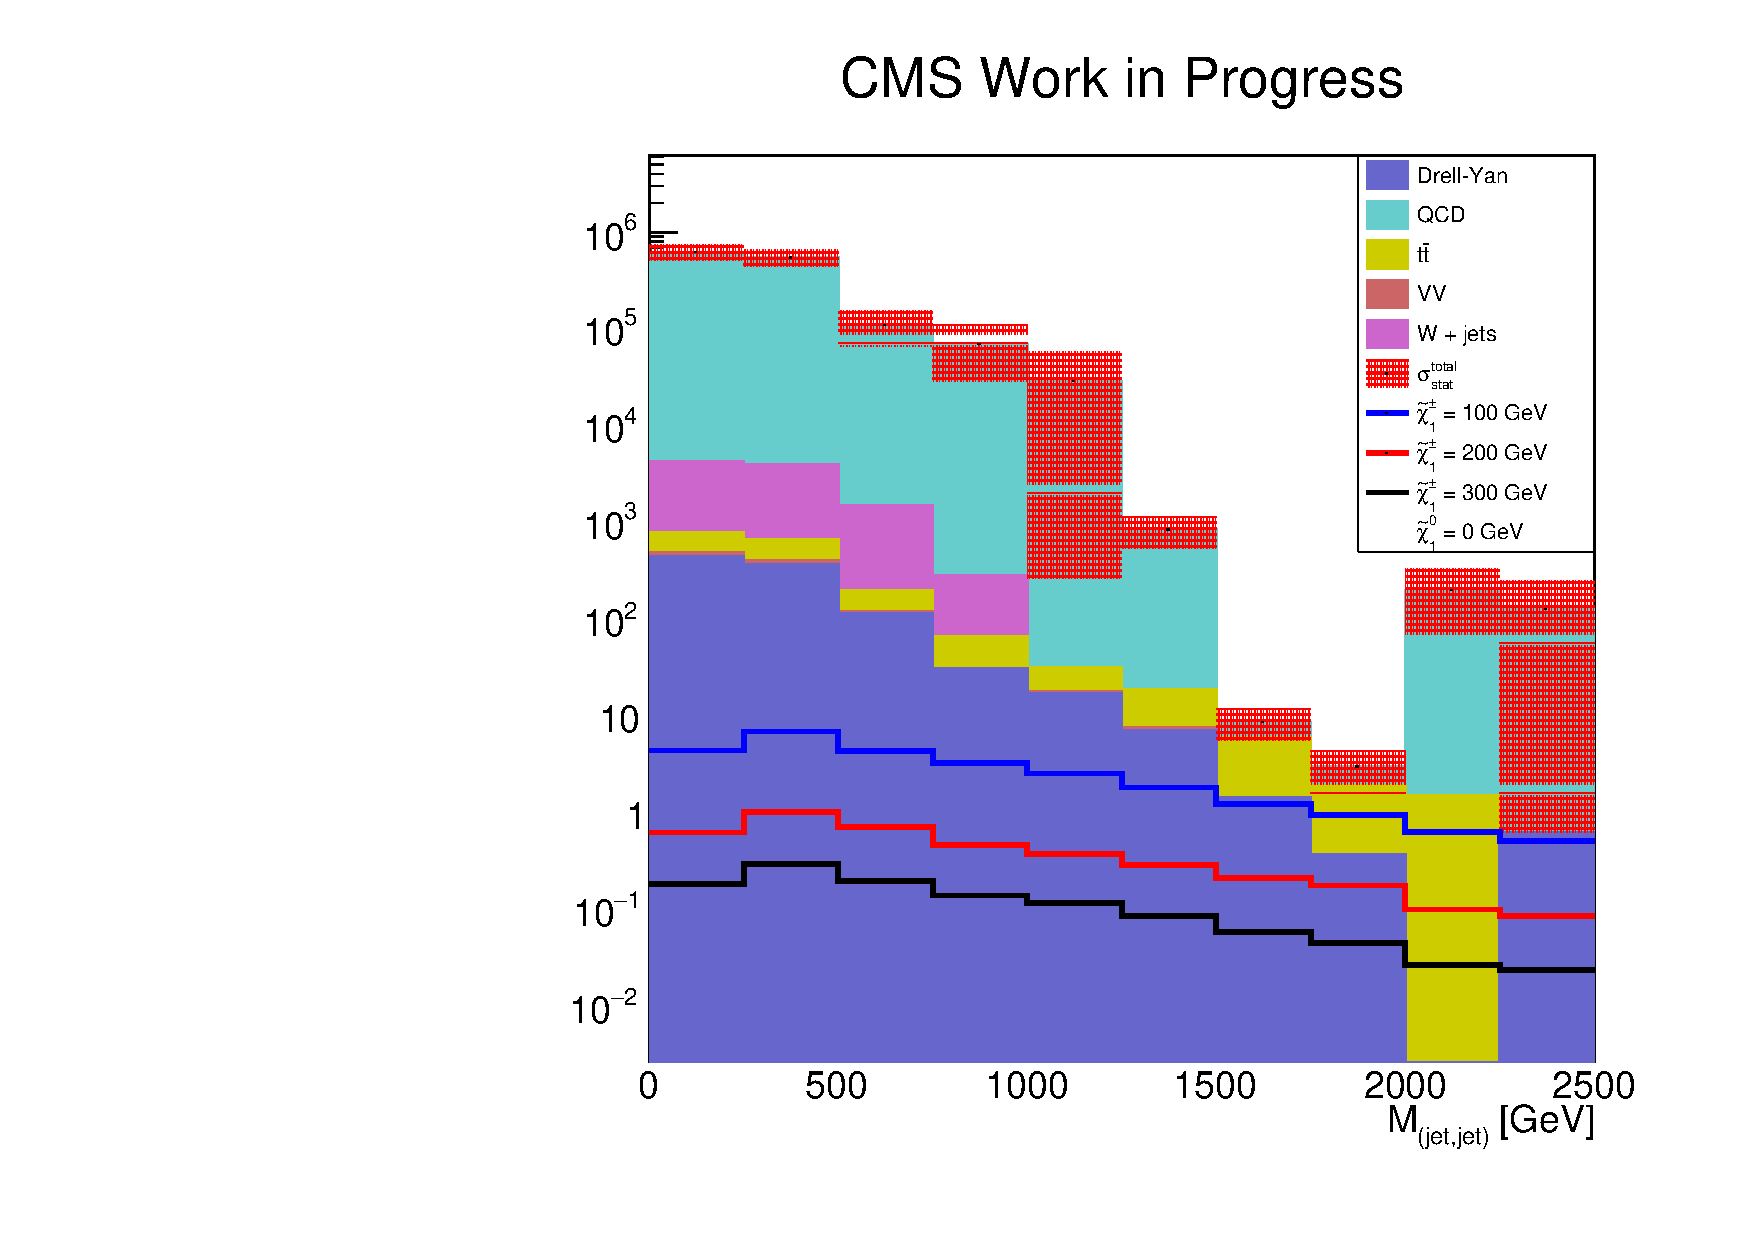
\includegraphics[width=0.5\textwidth]{analysis/pics/h_dijetinvariantmass_Taui2TightIso.pdf}
		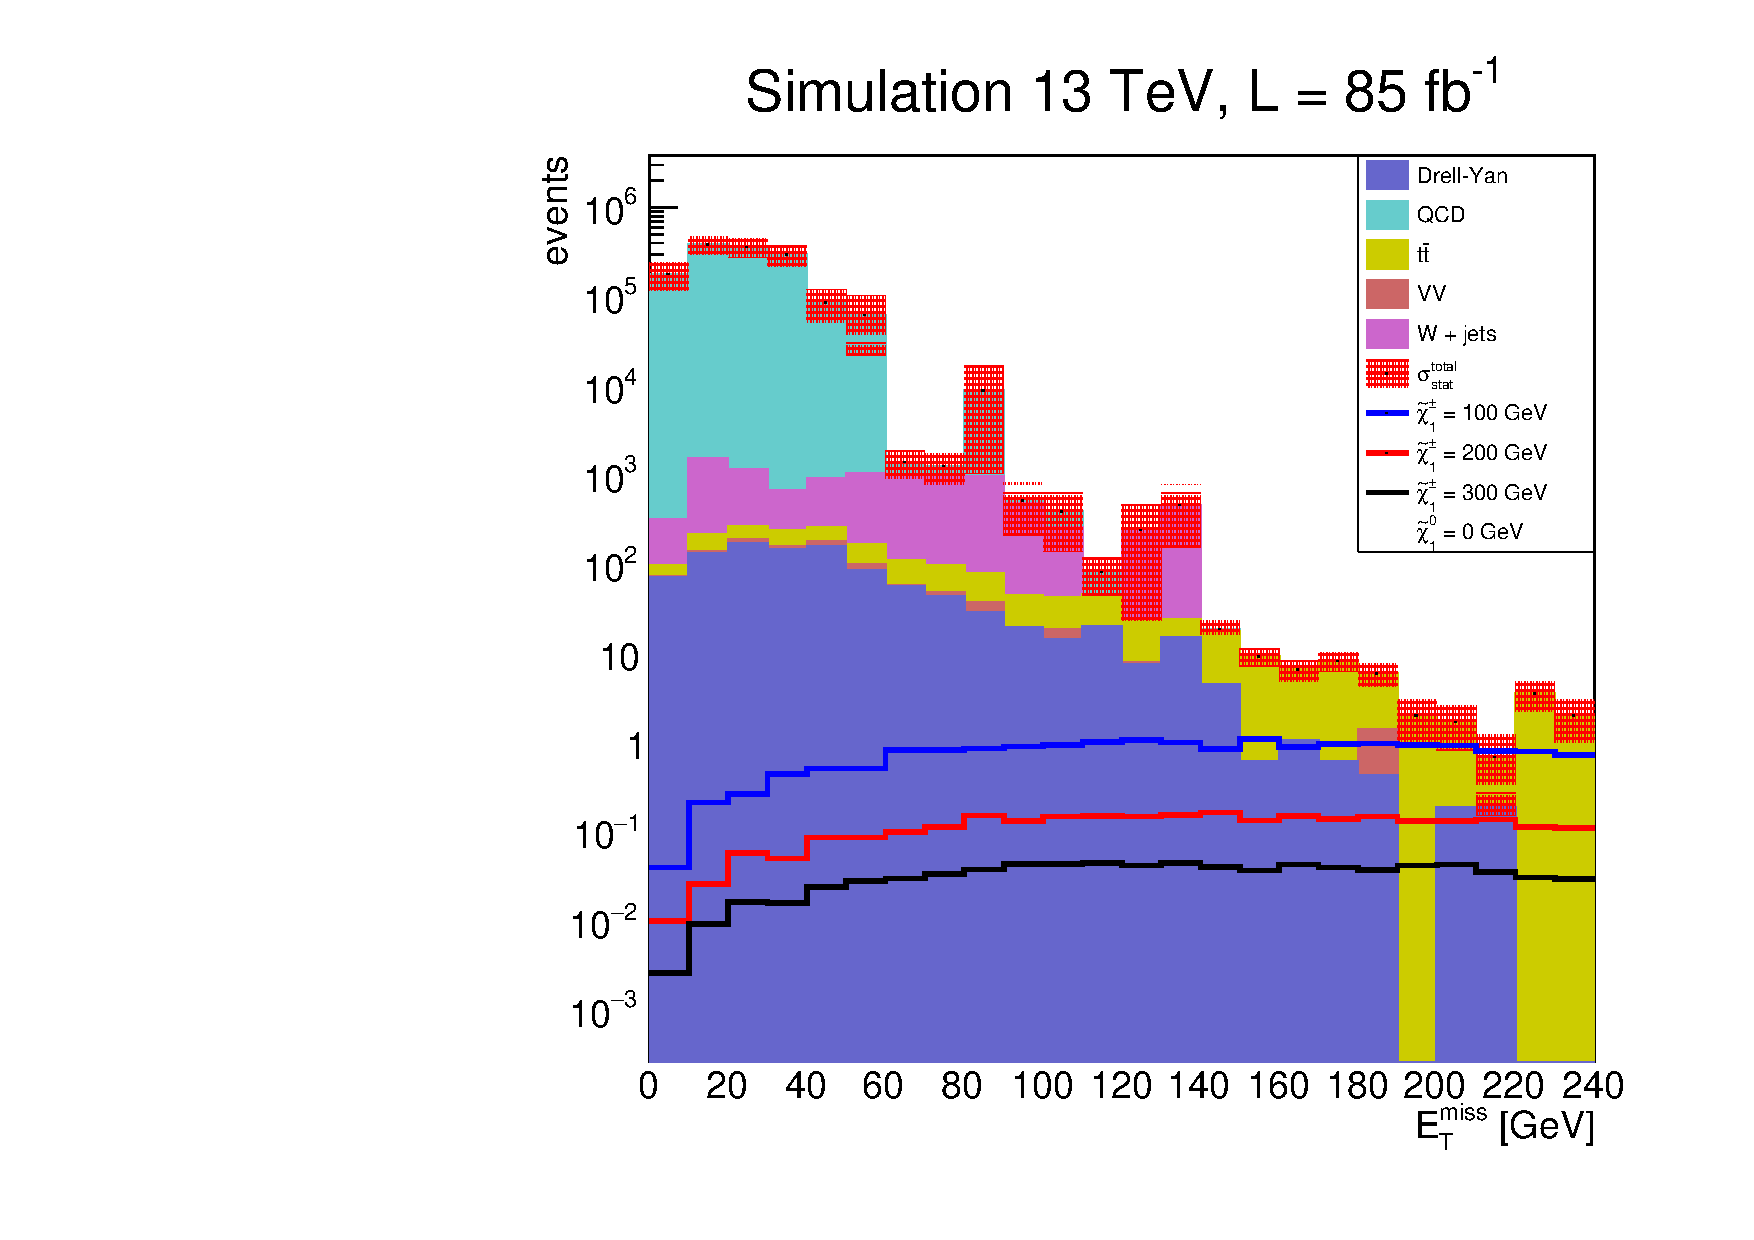
\includegraphics[width=0.5\textwidth]{analysis/pics/h_met_Taui2TightIso.pdf} 		
	\end{tabular}
	\caption{(Left) Di-jet invariant mass distribution and (Right) and \met distribution of selected signal and all MC background samples in signal region.}
	\label{fig::crplots1_Taui2TightIso_13tev}
\end{figure}

\begin{figure}[tbh!]
	\centering
	\begin{tabular}{cc}
		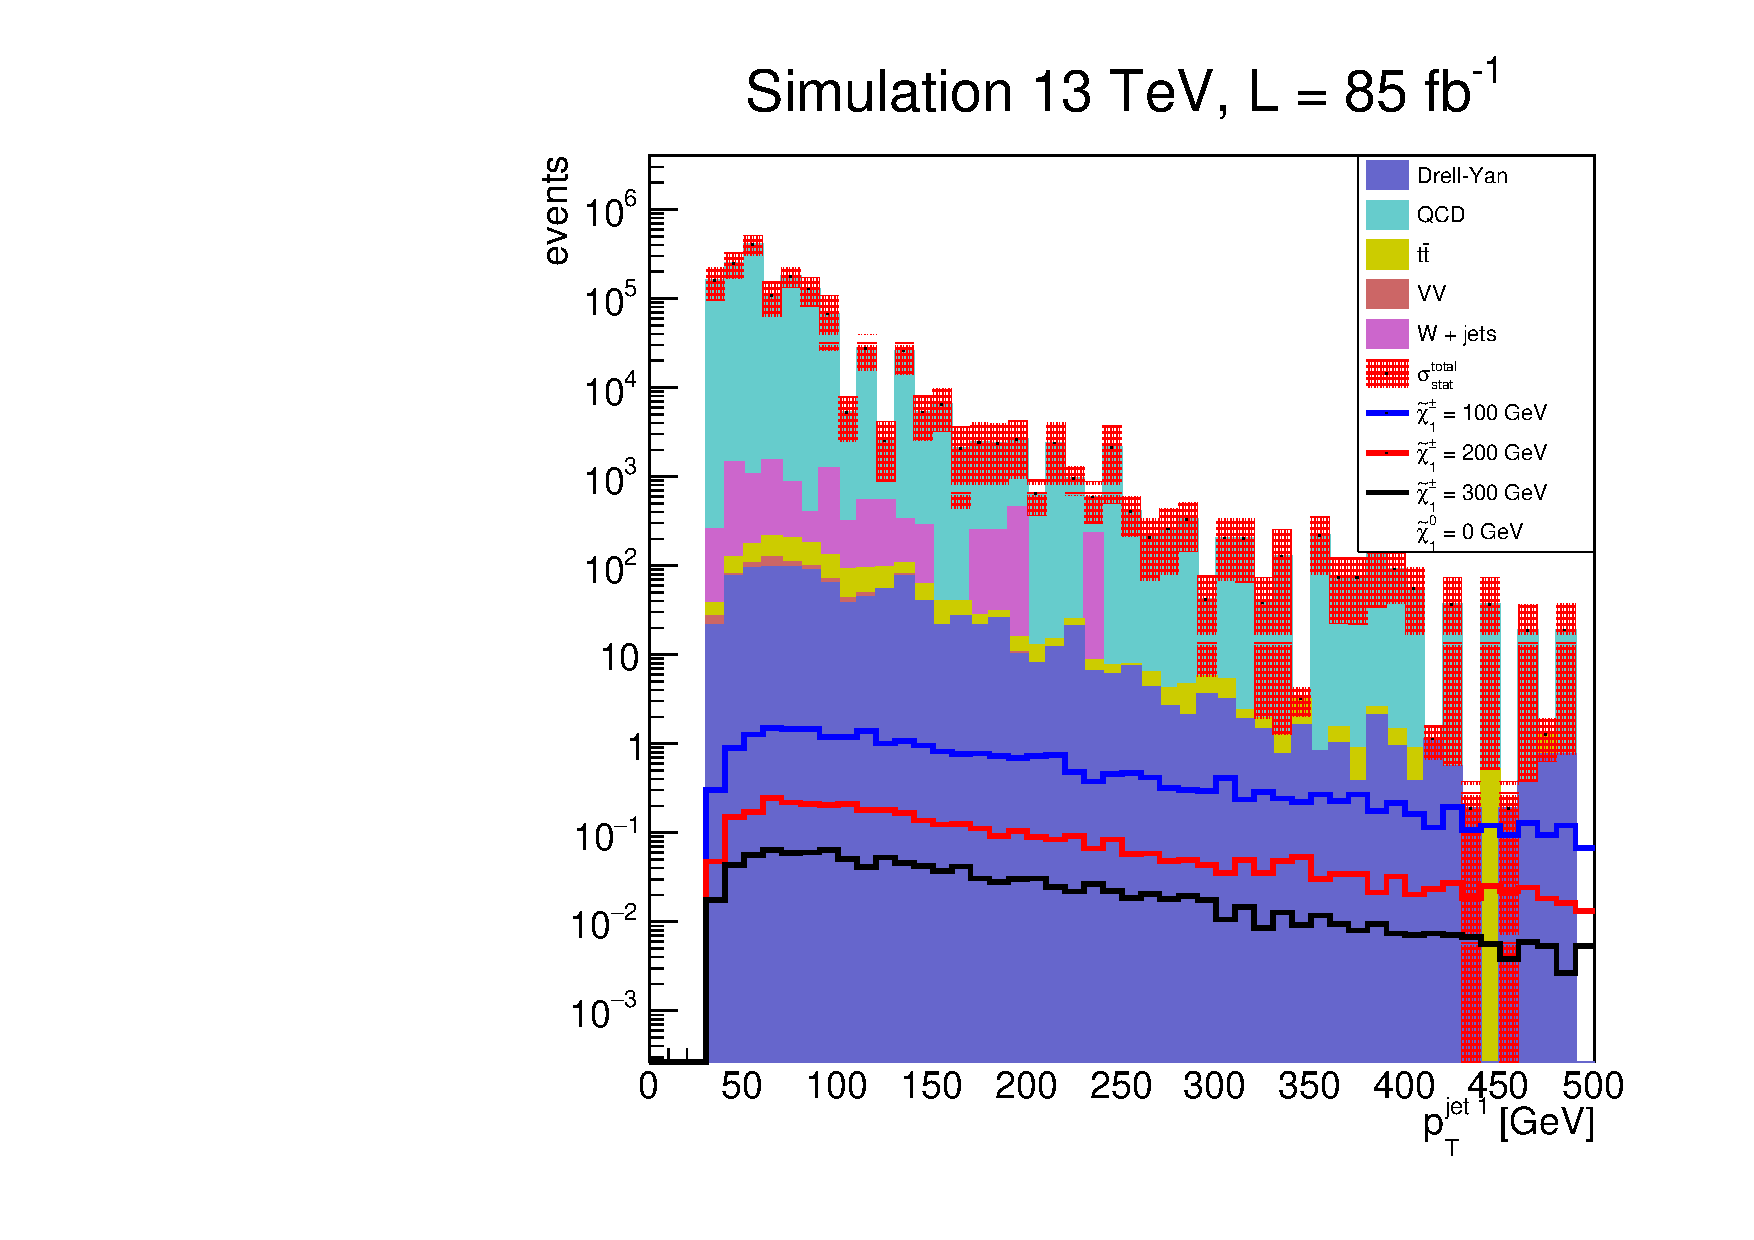
\includegraphics[width=0.5\textwidth]{analysis/pics/h_jet1pt_Taui2TightIso.pdf}
		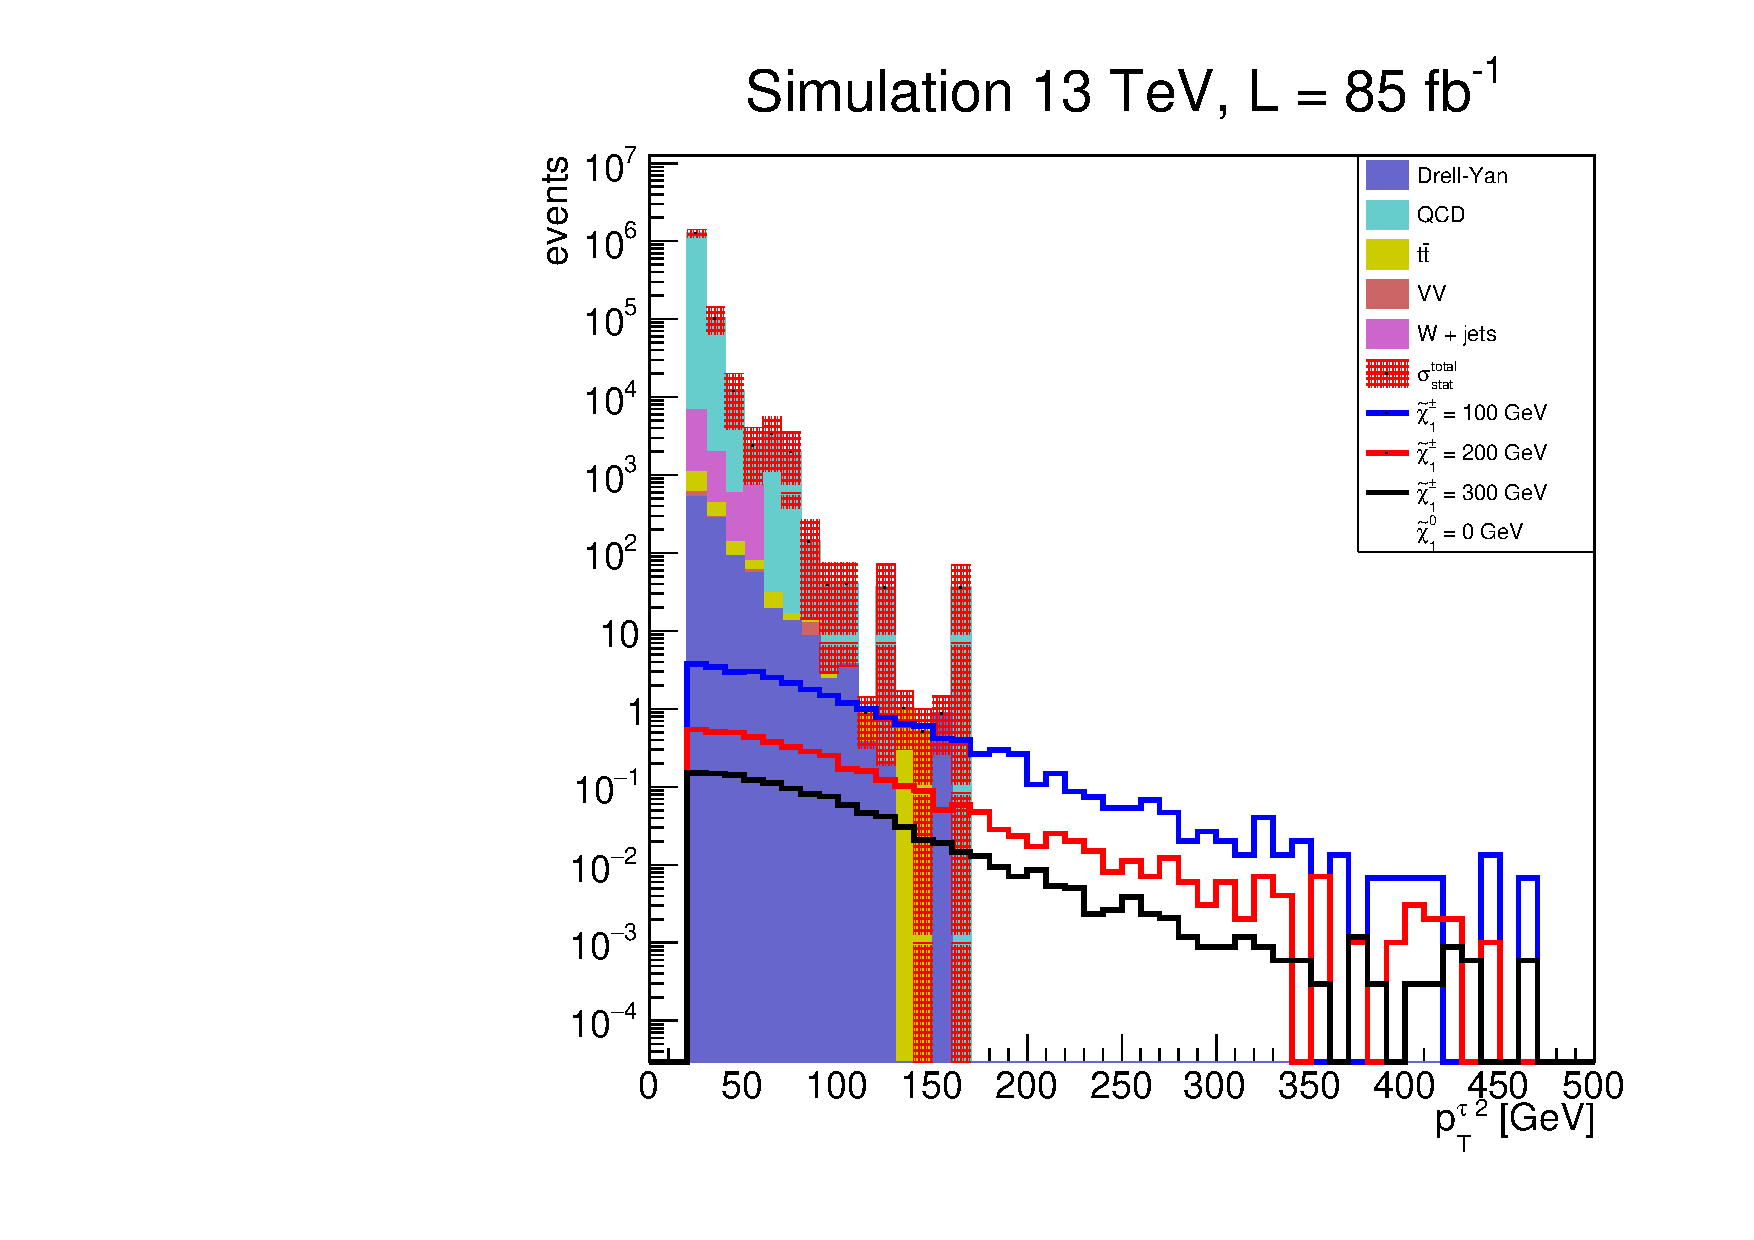
\includegraphics[width=0.5\textwidth]{analysis/pics/h_tau2pt_Taui2TightIso.pdf} 		
	\end{tabular}
	\caption{(Left) Leading jet \pt distribution and (Right) and second leading \hadtau \pt distribution of selected signal and all MC background samples in signal region.}
	\label{fig::crplots2_Taui2TightIso_13tev}
\end{figure}

\subsection*{Control region 2}

\FloatBarrier

2 tight-isolated \hadtau, inverted VBF selection

\begin{figure}[tbh!]
	\centering
	\begin{tabular}{cc}
		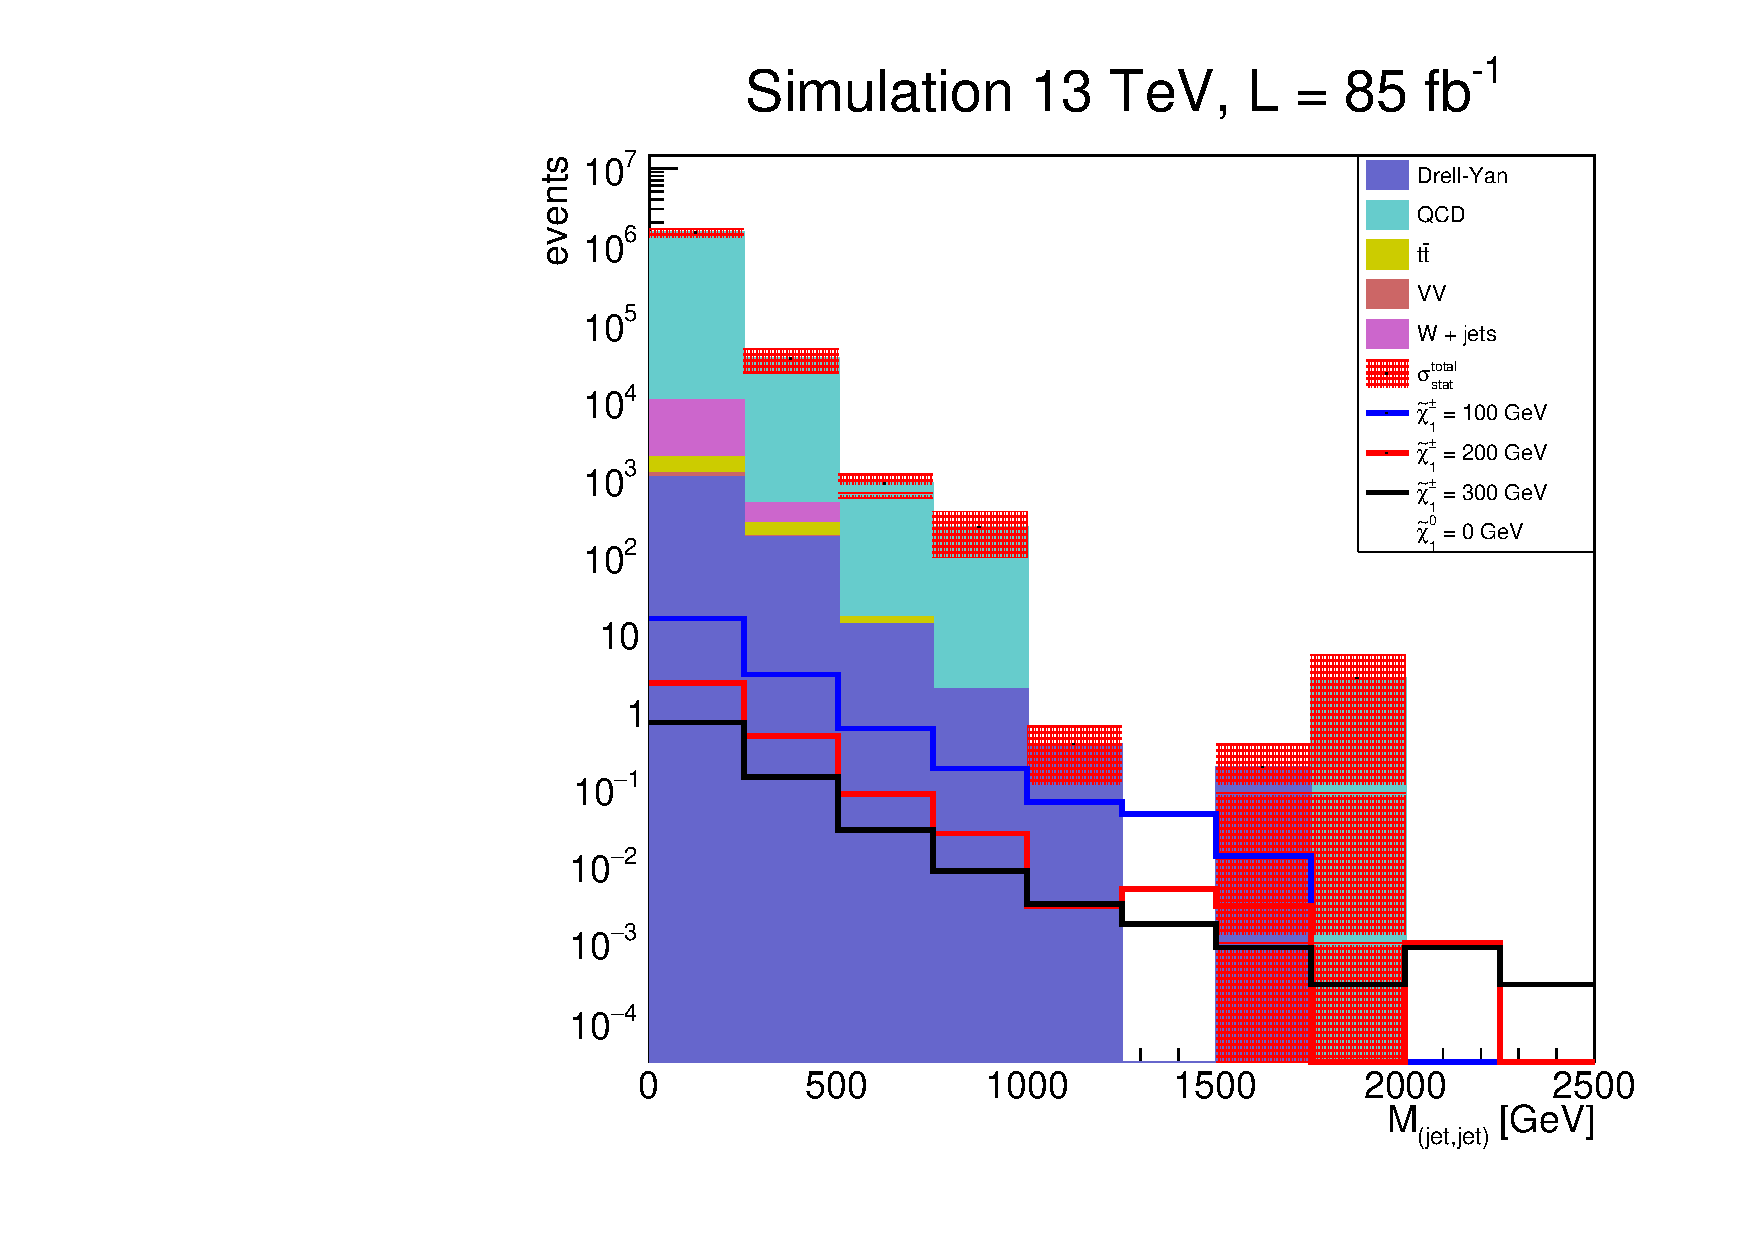
\includegraphics[width=0.5\textwidth]{analysis/pics/h_dijetinvariantmass_Tau2TightIsoVBFInverted.pdf}
		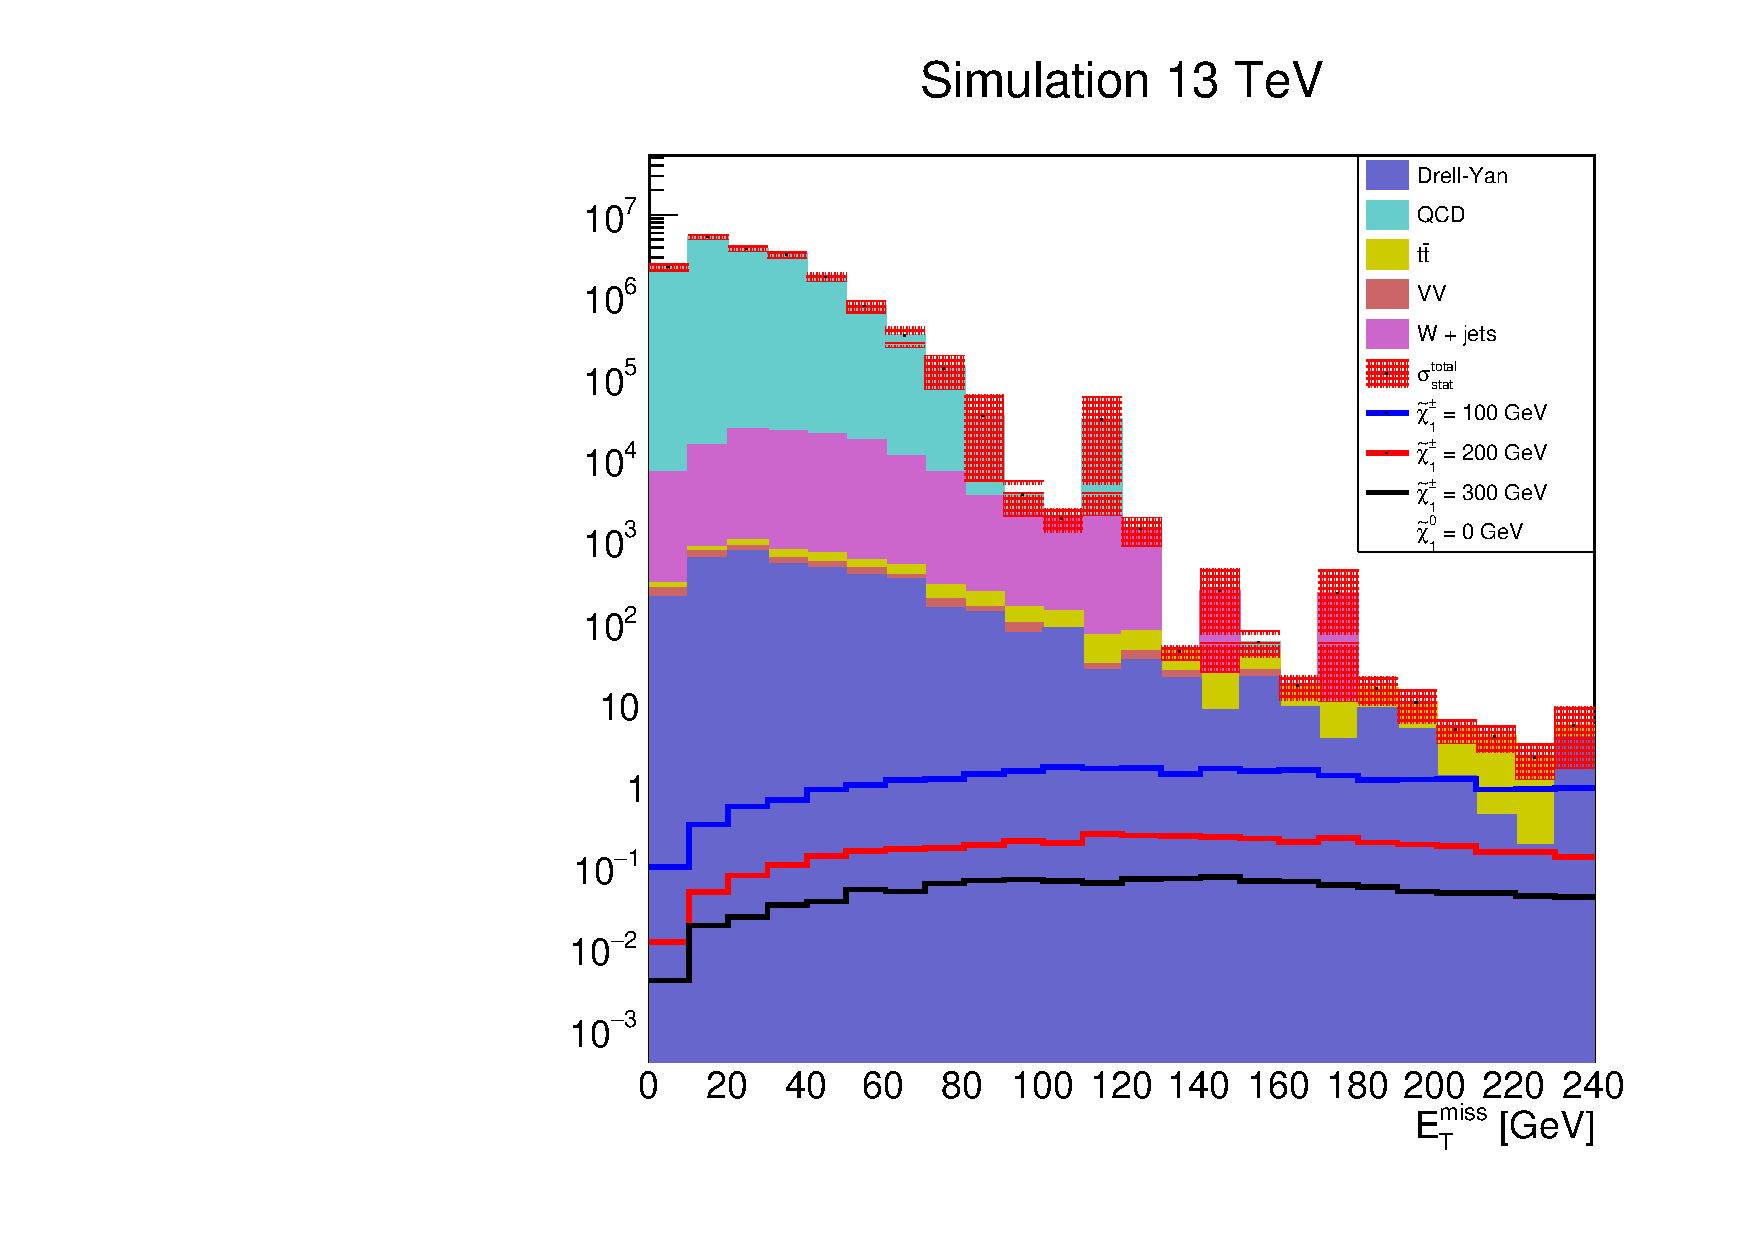
\includegraphics[width=0.5\textwidth]{analysis/pics/h_met_Tau2TightIsoVBFInverted.pdf} 		
	\end{tabular}
	\caption{(Left) Di-jet invariant mass distribution and (Right) and \met distribution of selected signal and all MC background samples in control region 2.}
	\label{fig::crplots1_Tau2TightIsoVBFInverted_13tev}
\end{figure}

\begin{figure}[tbh!]
	\centering
	\begin{tabular}{cc}
		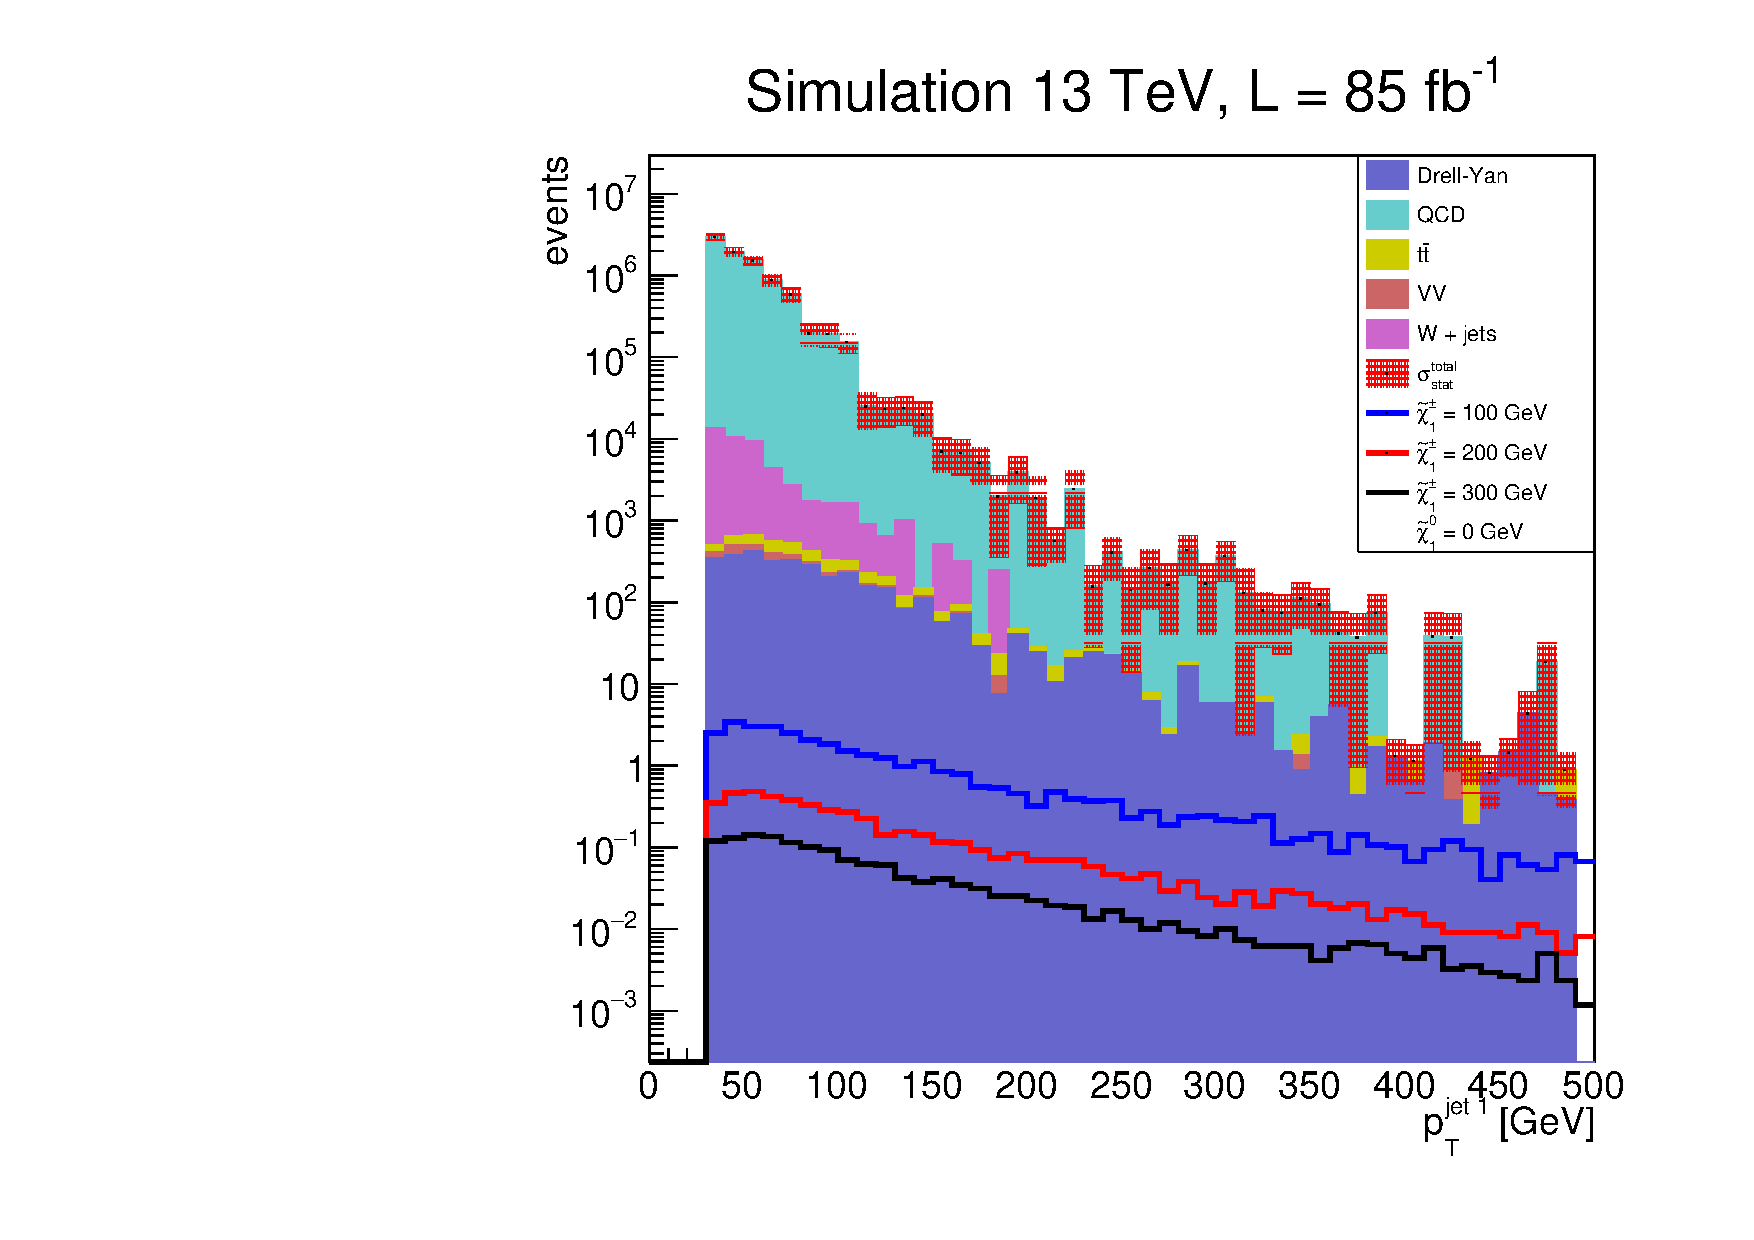
\includegraphics[width=0.5\textwidth]{analysis/pics/h_jet1pt_Tau2TightIsoVBFInverted.pdf}
		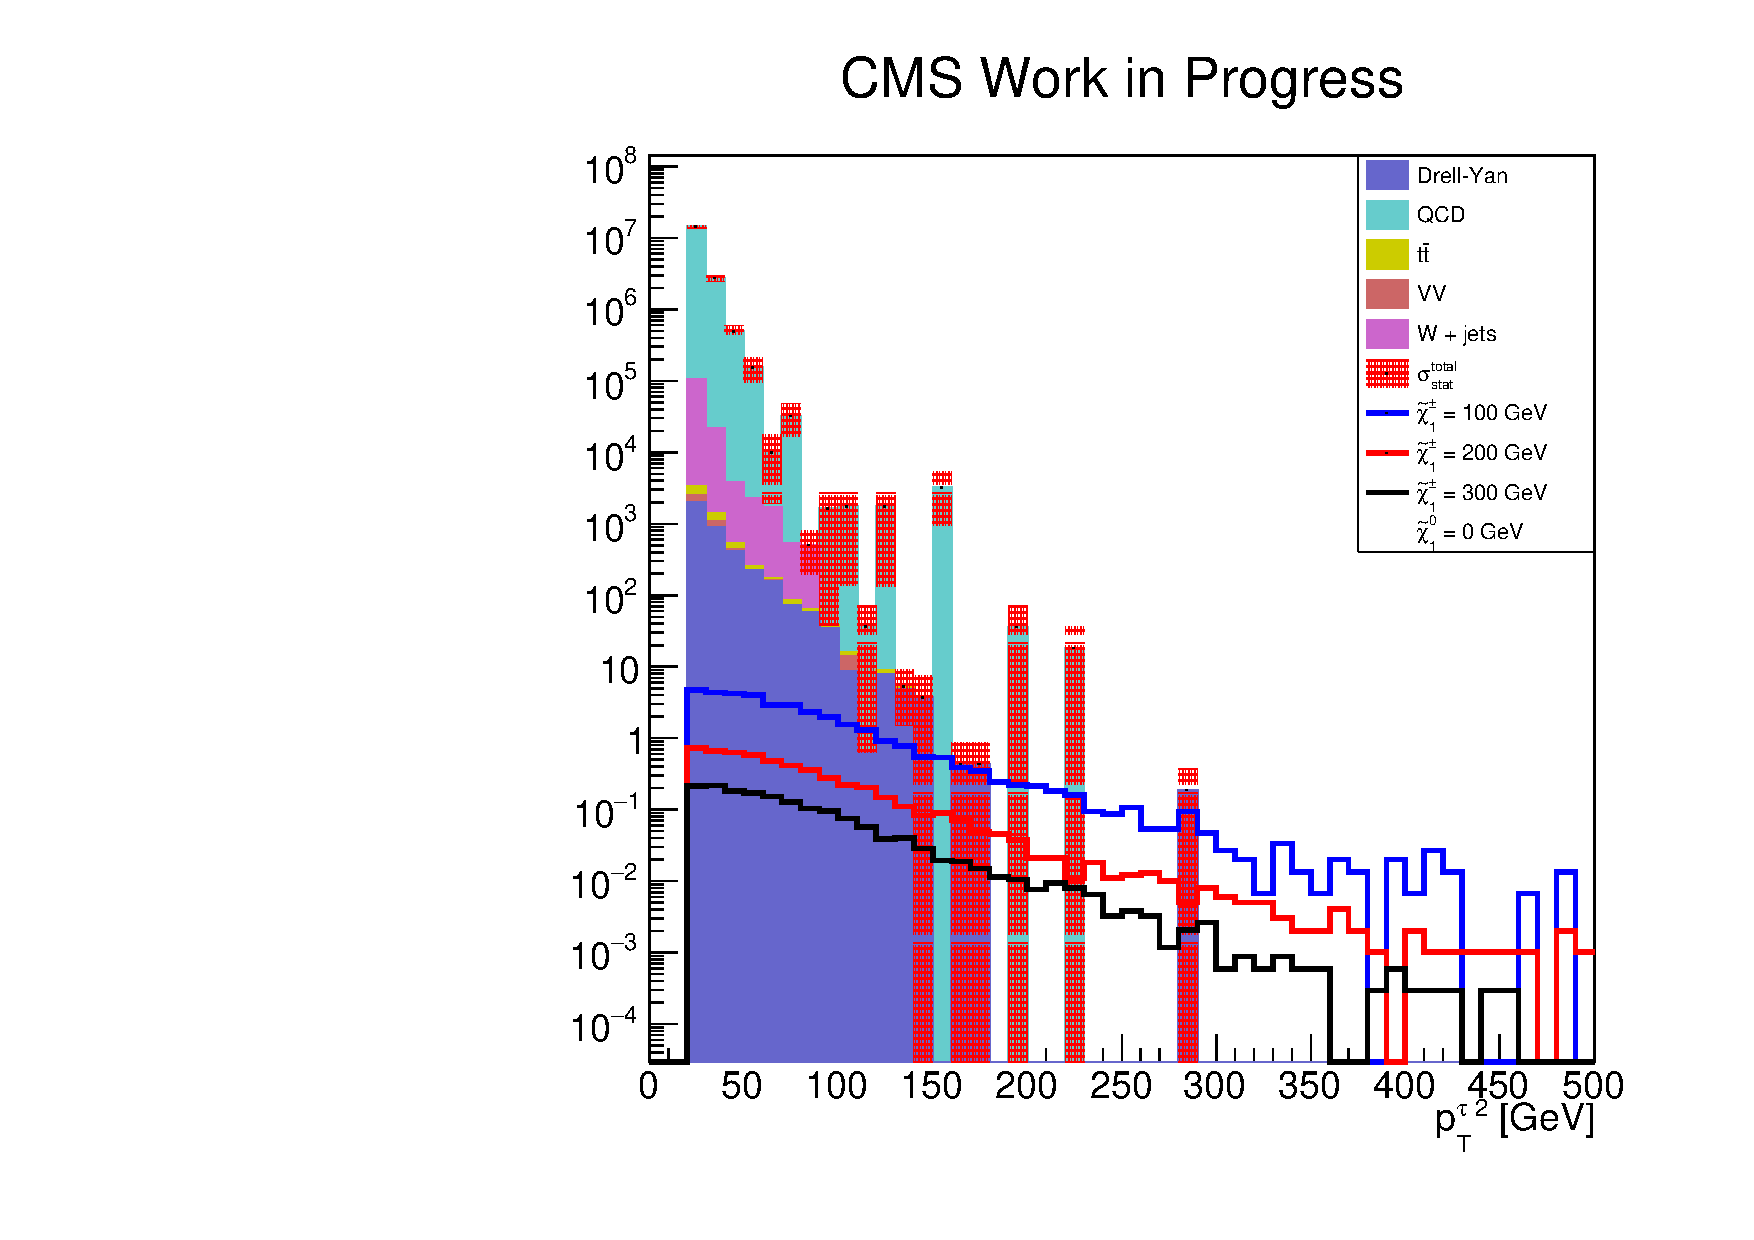
\includegraphics[width=0.5\textwidth]{analysis/pics/h_tau2pt_Tau2TightIsoVBFInverted.pdf} 		
	\end{tabular}
	\caption{(Left) Leading jet \pt distribution and (Right) and second leading \hadtau \pt distribution of selected signal and all MC background samples in control region 2.}
	\label{fig::crplots2_Taui2TightIsoVBFInverted_13tev}
\end{figure}

\subsection*{Control region 3}

\FloatBarrier

2 loose-isolated \hadtau (inclusive)

\begin{figure}[tbh!]
	\centering
	\begin{tabular}{cc}
		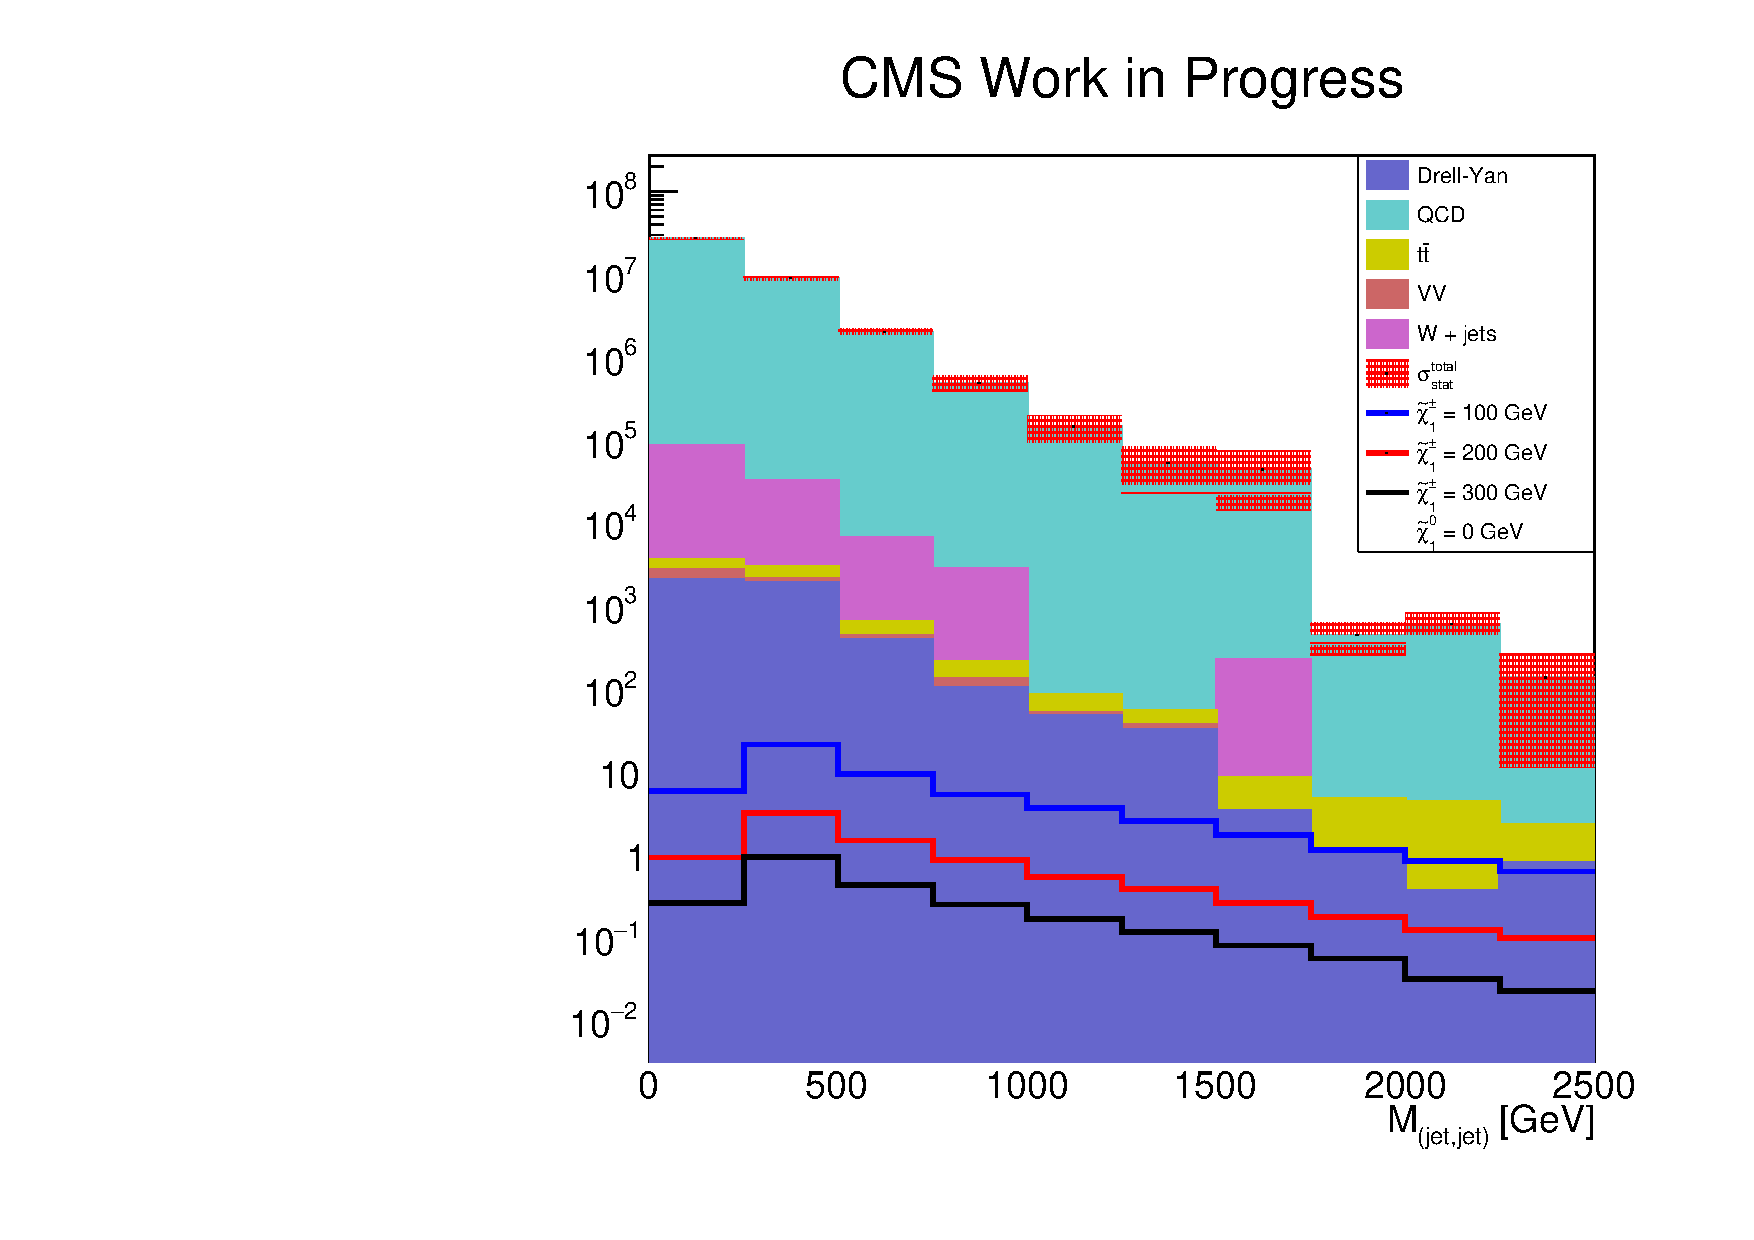
\includegraphics[width=0.5\textwidth]{analysis/pics/h_dijetinvariantmass_Tau2LooseIsoInclusive.pdf}
		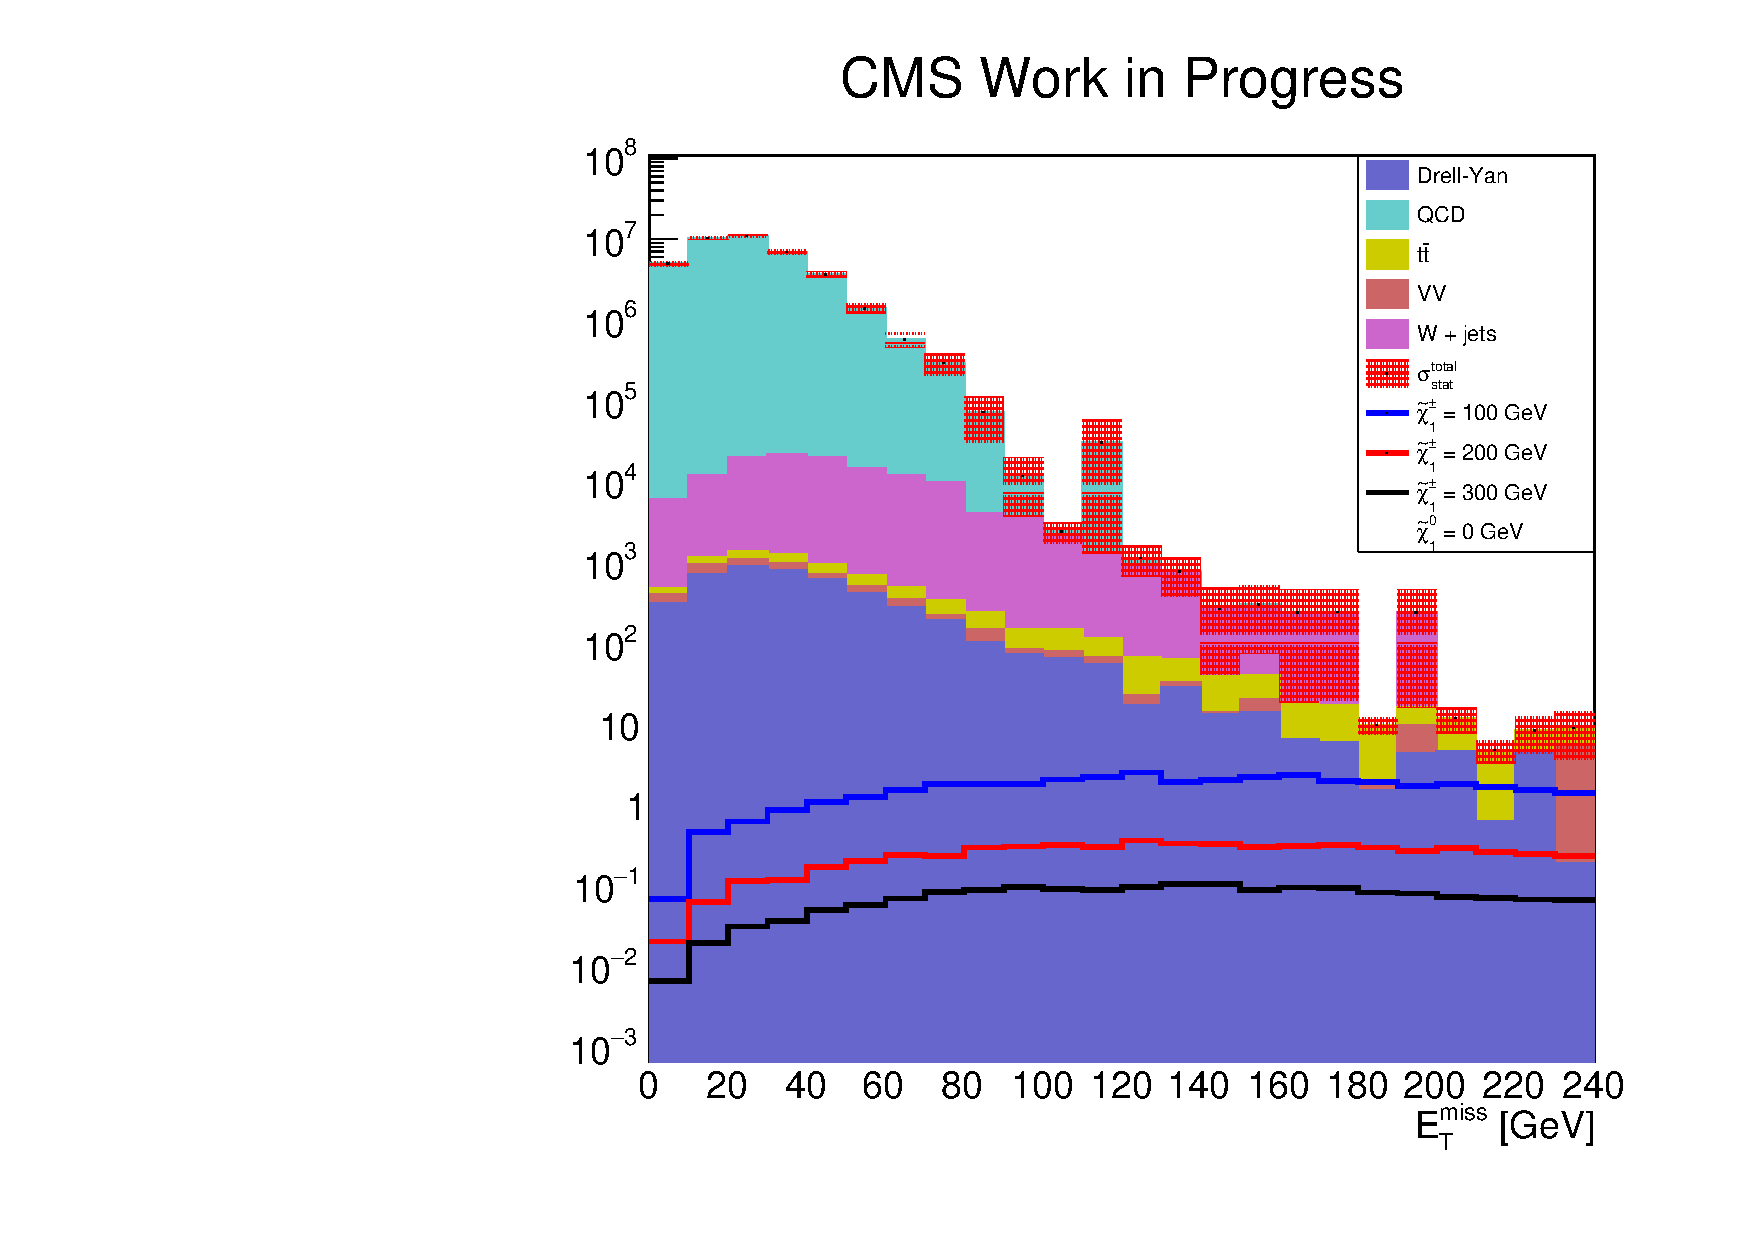
\includegraphics[width=0.5\textwidth]{analysis/pics/h_met_Tau2LooseIsoInclusive.pdf} 		
	\end{tabular}
	\caption{(Left) Di-jet invariant mass distribution and (Right) and \met distribution of selected signal and all MC background samples in control region 3.}
	\label{fig::crplots1_Tau2LooseIsoInclusive_13tev}
\end{figure}

\begin{figure}[tbh!]
	\centering
	\begin{tabular}{cc}
		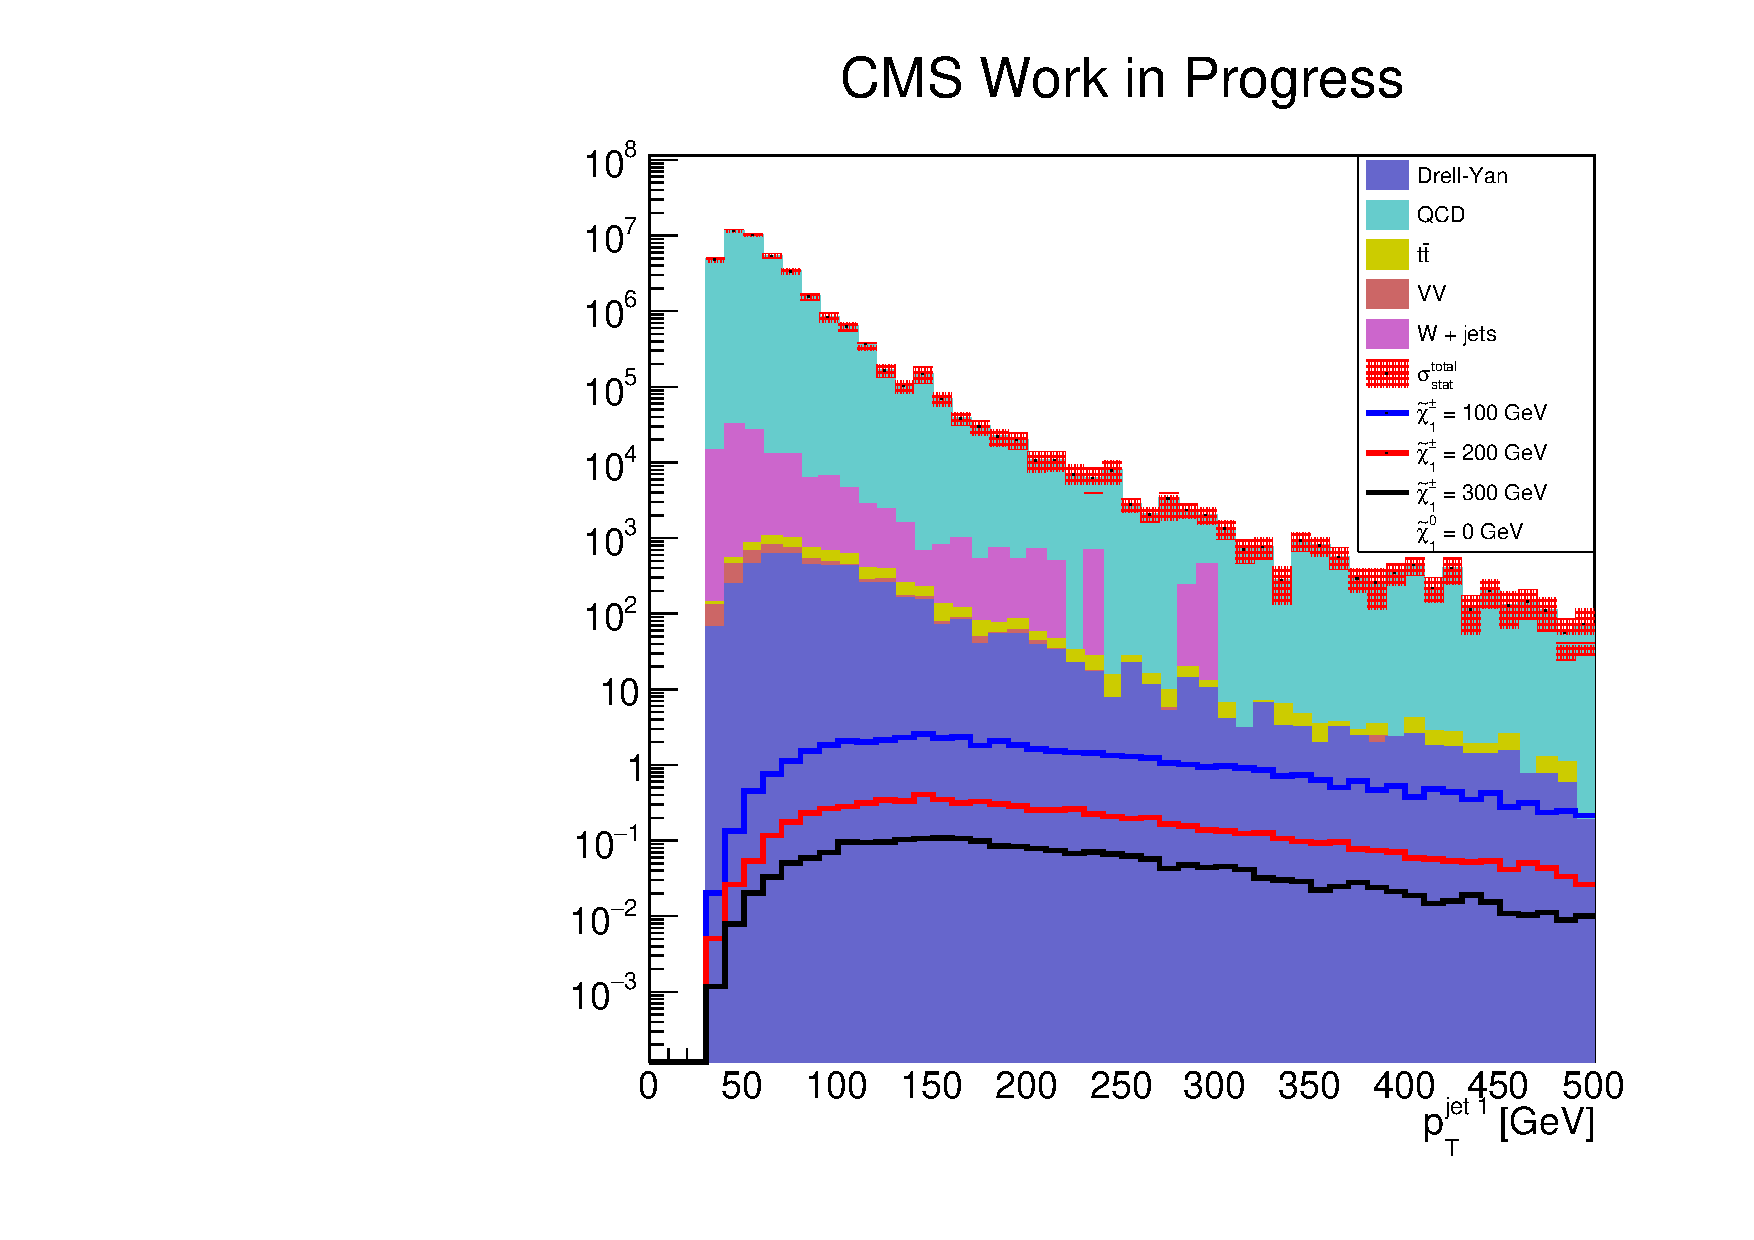
\includegraphics[width=0.5\textwidth]{analysis/pics/h_jet1pt_Tau2LooseIsoInclusive.pdf}
		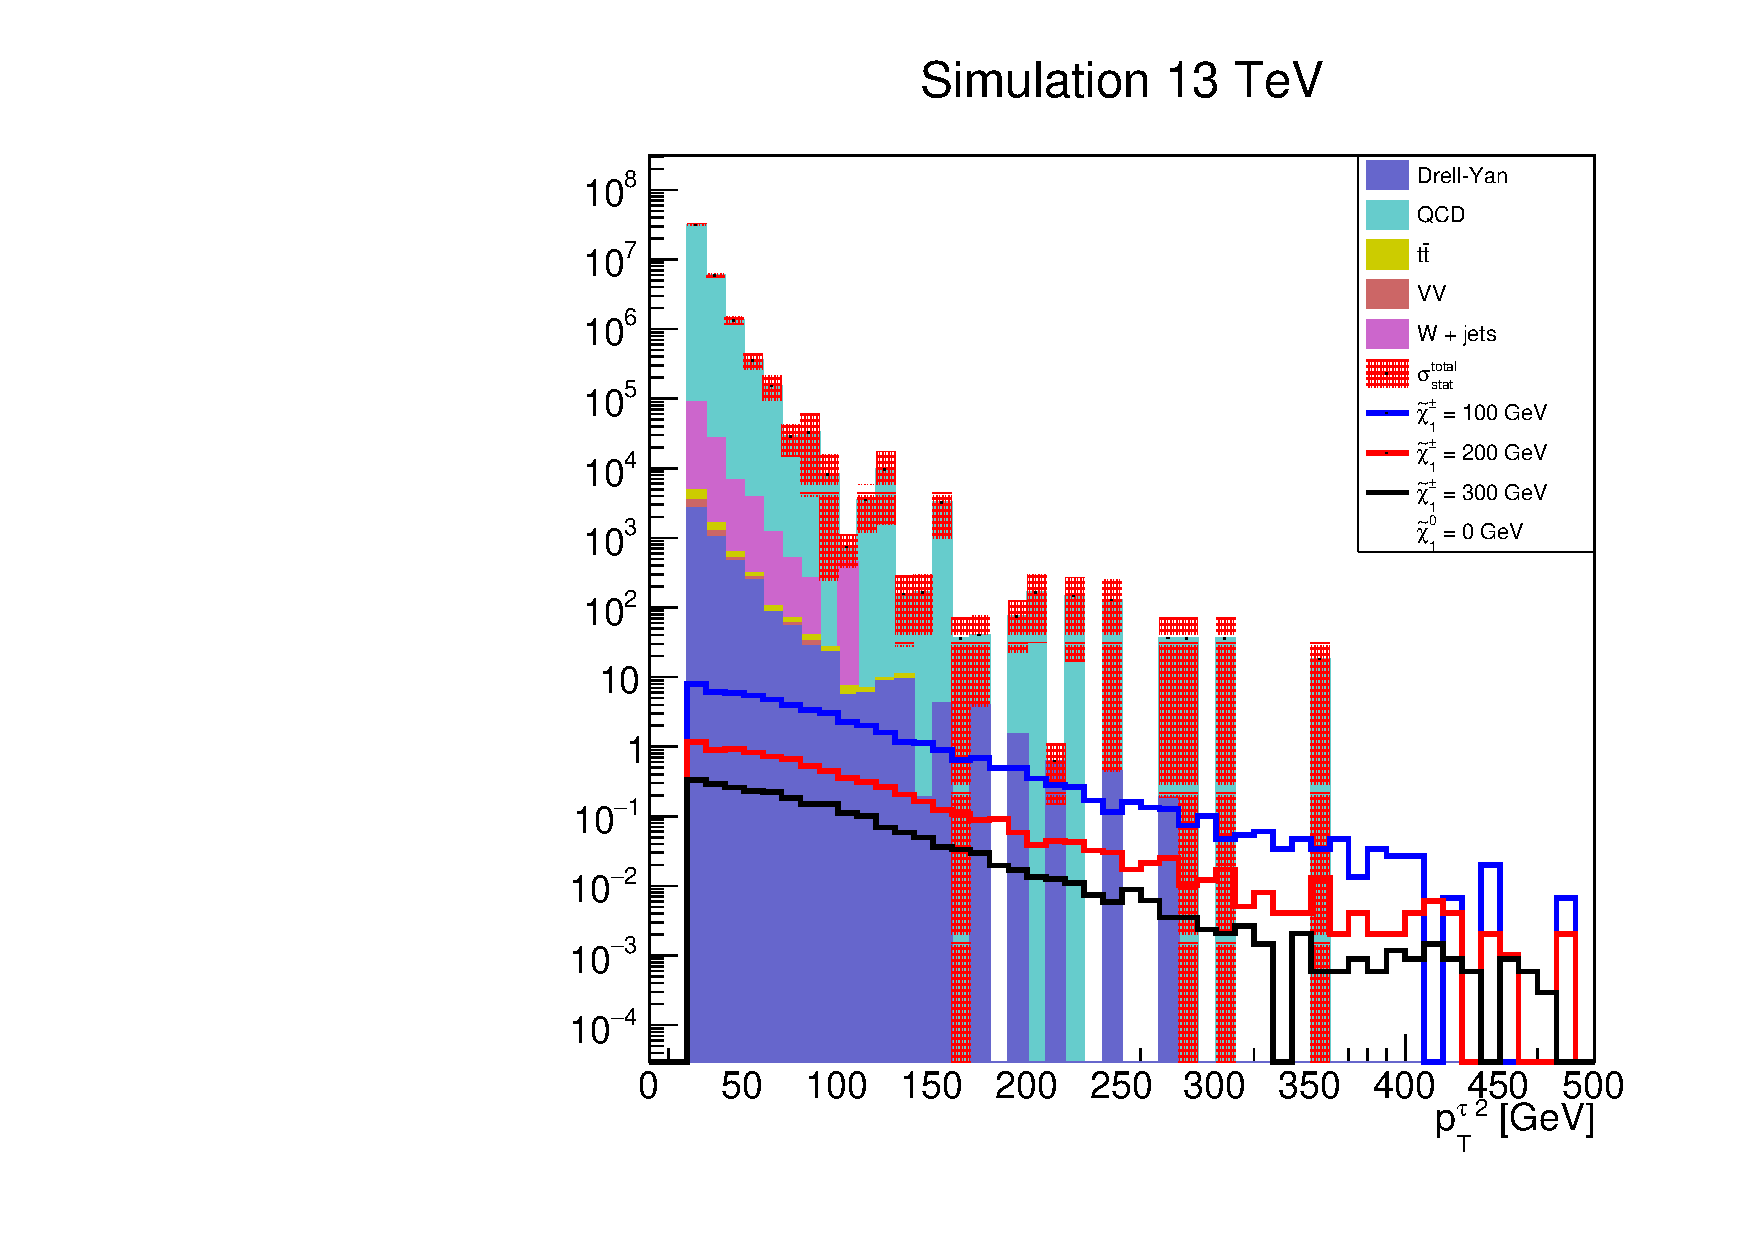
\includegraphics[width=0.5\textwidth]{analysis/pics/h_tau2pt_Tau2LooseIsoInclusive.pdf} 		
	\end{tabular}
	\caption{(Left) Leading jet \pt distribution and (Right) and second leading \hadtau \pt distribution of selected signal and all MC background samples in control region 3.}
	\label{fig::crplots2_Tau2LooseIsoInclusive_13tev}
\end{figure}

\subsection*{Control region 4}

\FloatBarrier

2 loose-isolated \hadtau (inclusive), inverted VBF selection

\begin{figure}[tbh!]
	\centering
	\begin{tabular}{cc}
		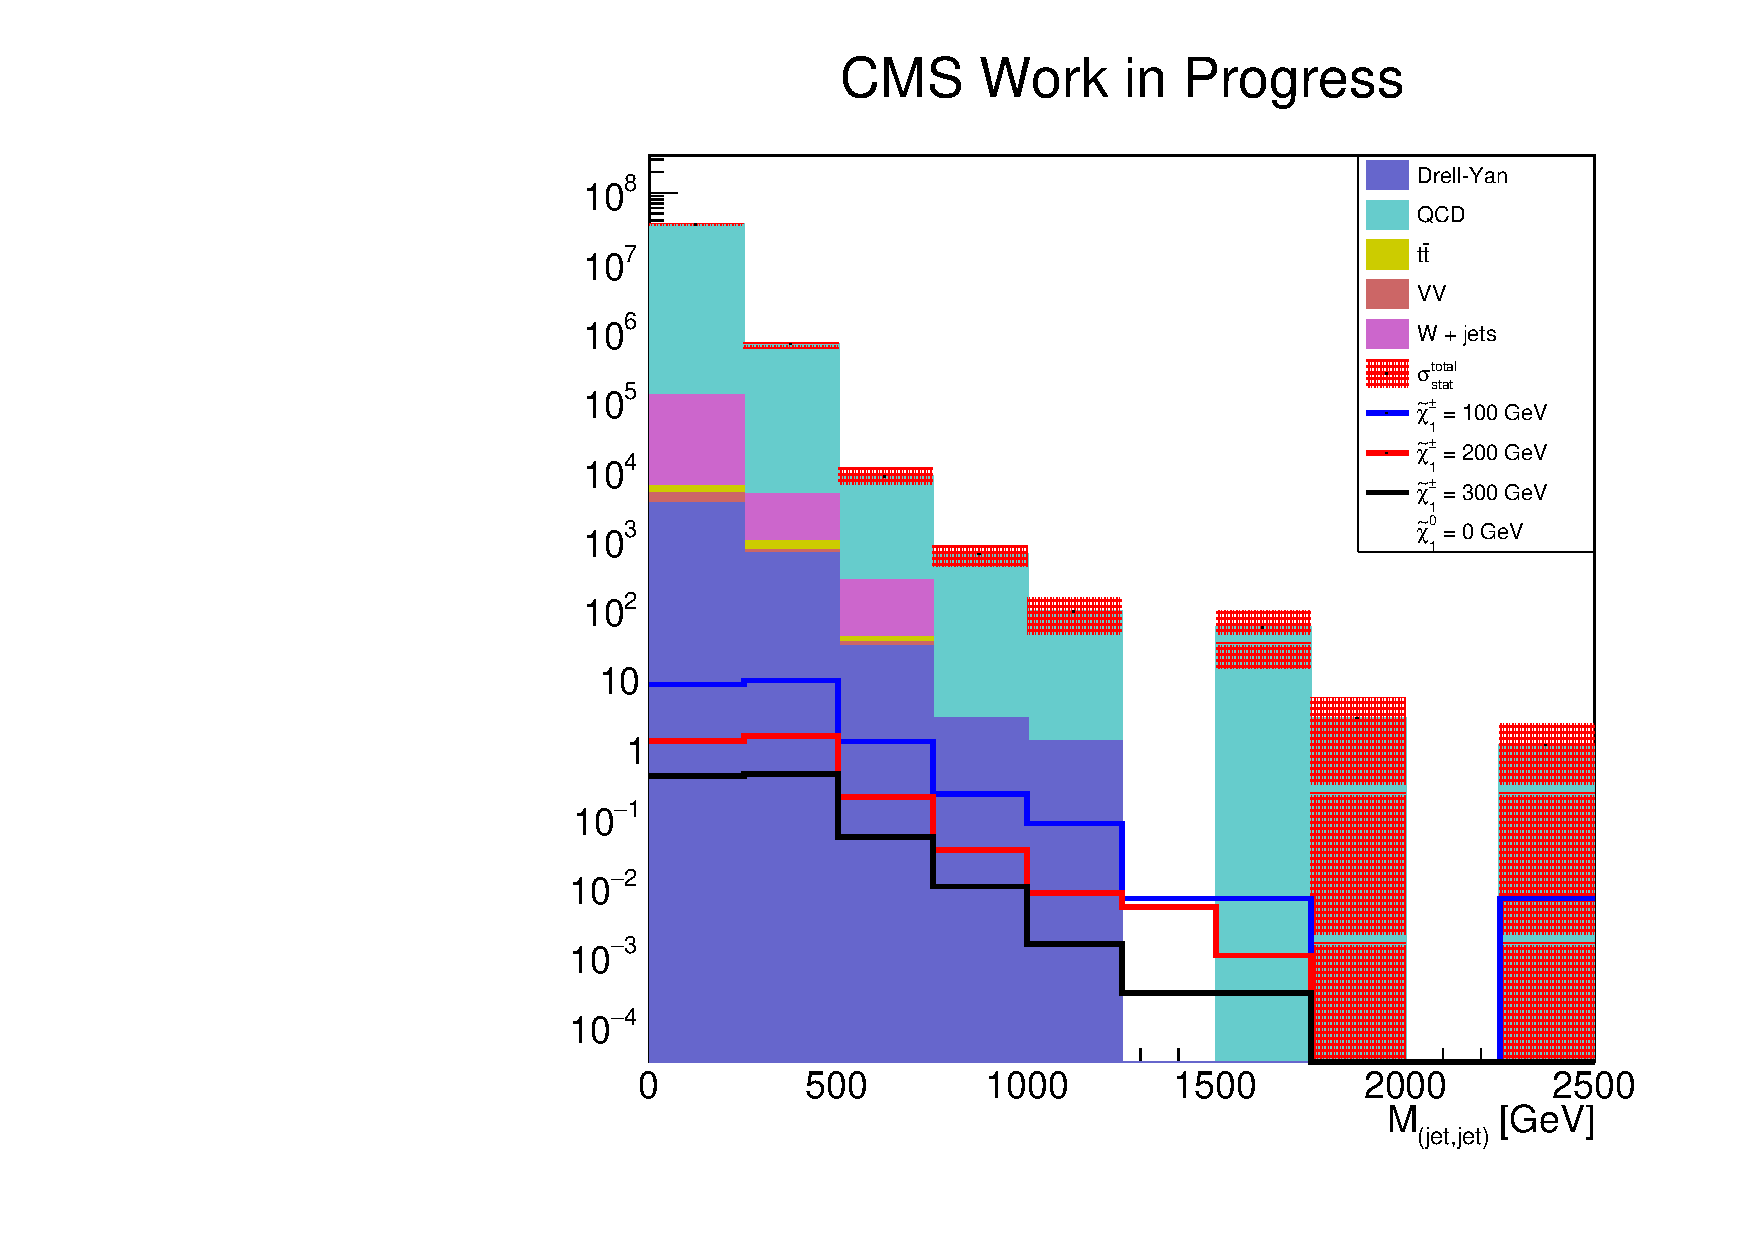
\includegraphics[width=0.5\textwidth]{analysis/pics/h_dijetinvariantmass_Tau2LooseIsoInclusiveVBFInverted.pdf}
		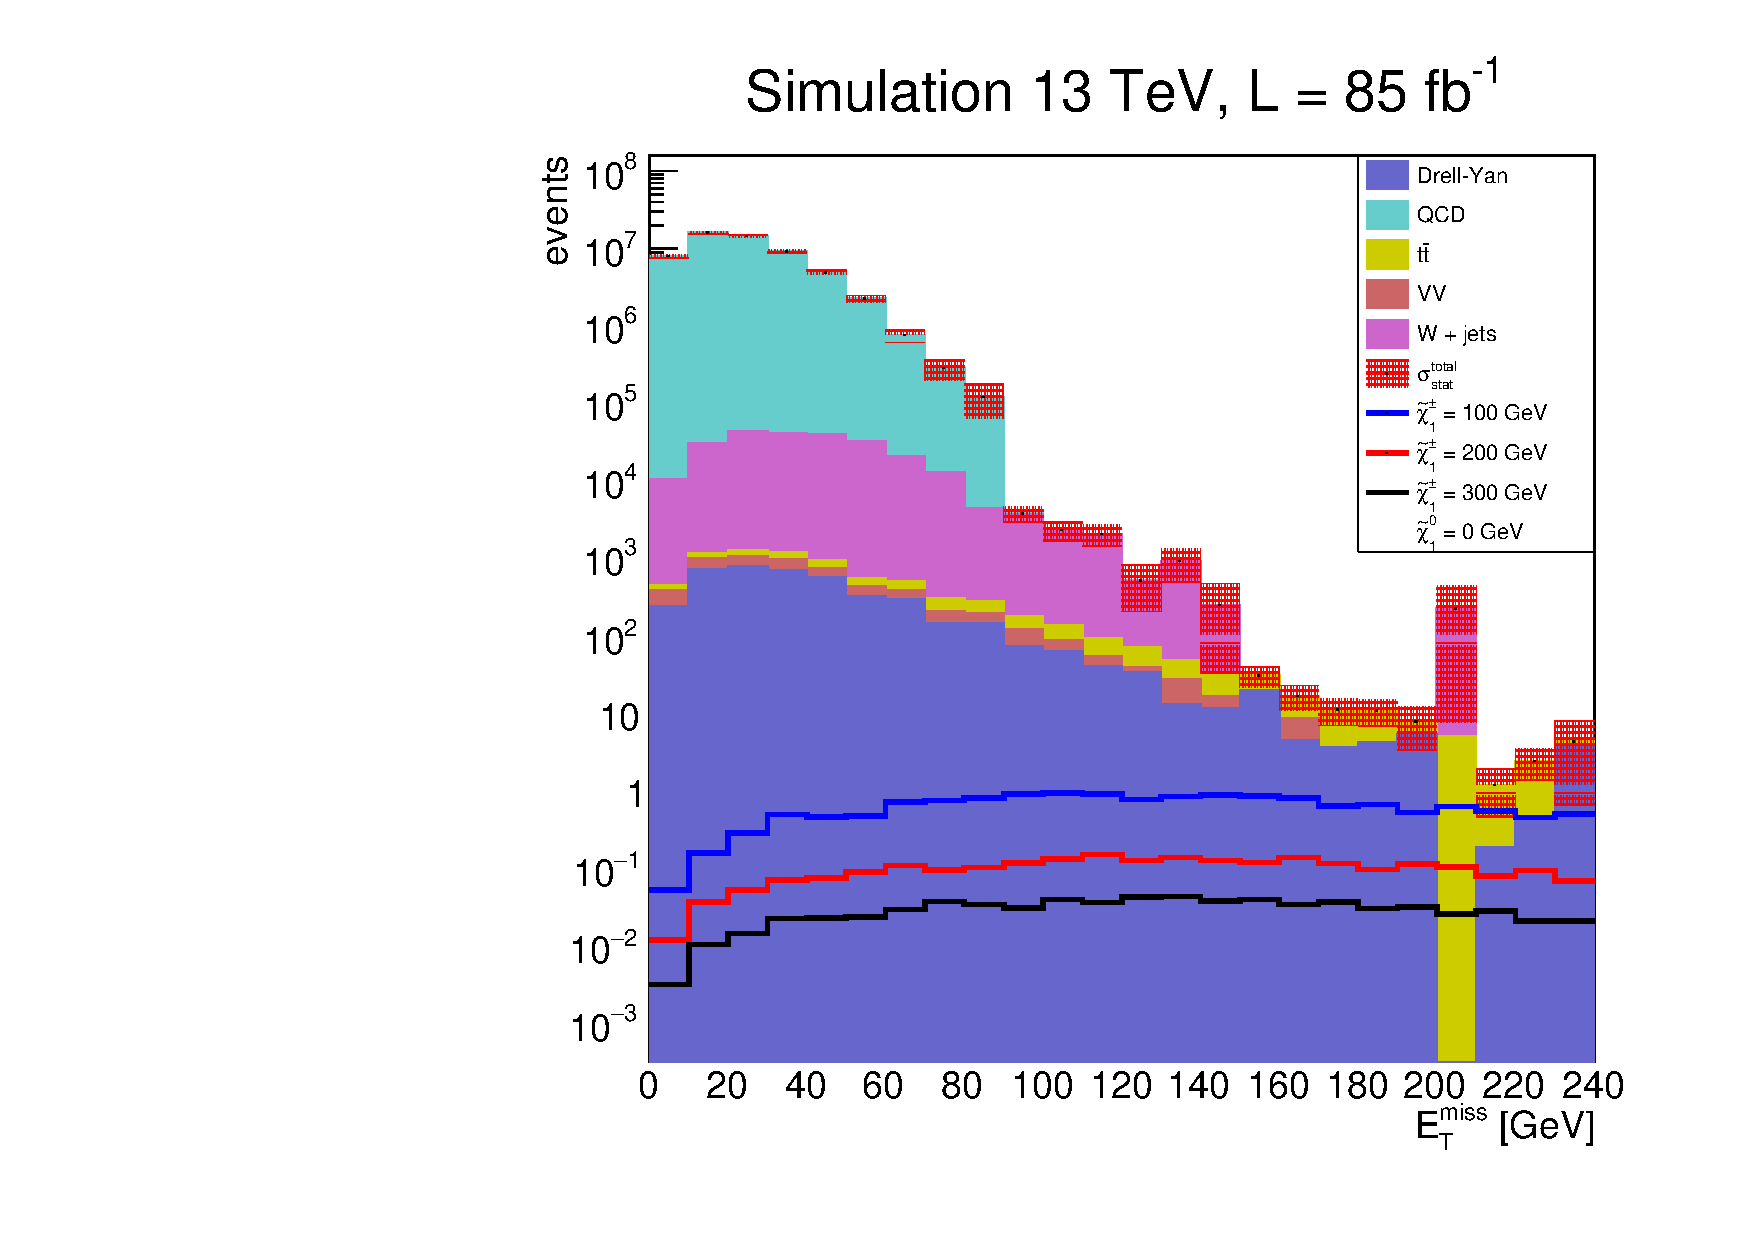
\includegraphics[width=0.5\textwidth]{analysis/pics/h_met_Tau2LooseIsoInclusiveVBFInverted.pdf} 		
	\end{tabular}
	\caption{(Left) Di-jet invariant mass distribution and (Right) and \met distribution of selected signal and all MC background samples in control region 4.}
	\label{fig::crplots1_Tau2LooseIsoInclusiveVBFInverted_13tev}
\end{figure}

\begin{figure}[tbh!]
	\centering
	\begin{tabular}{cc}
		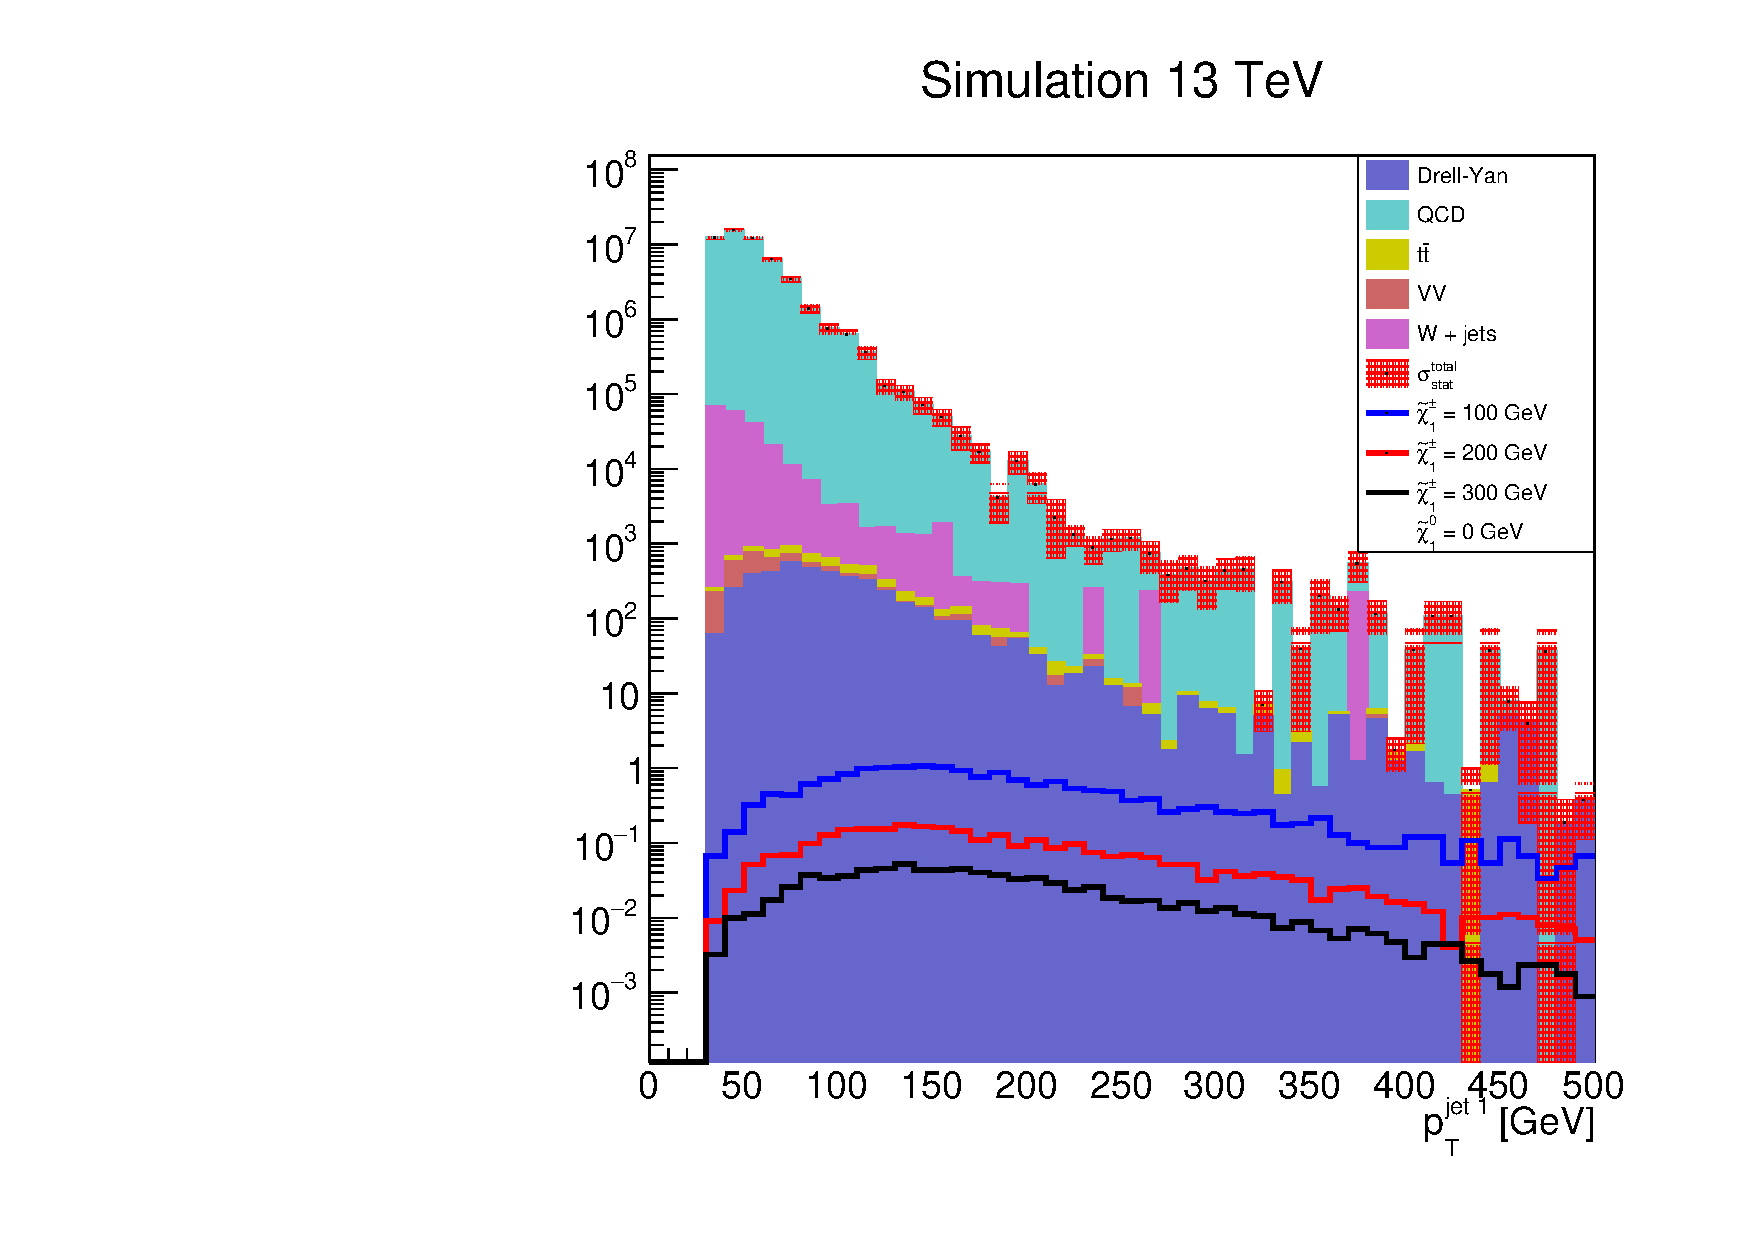
\includegraphics[width=0.5\textwidth]{analysis/pics/h_jet1pt_Tau2LooseIsoInclusiveVBFInverted.pdf}
		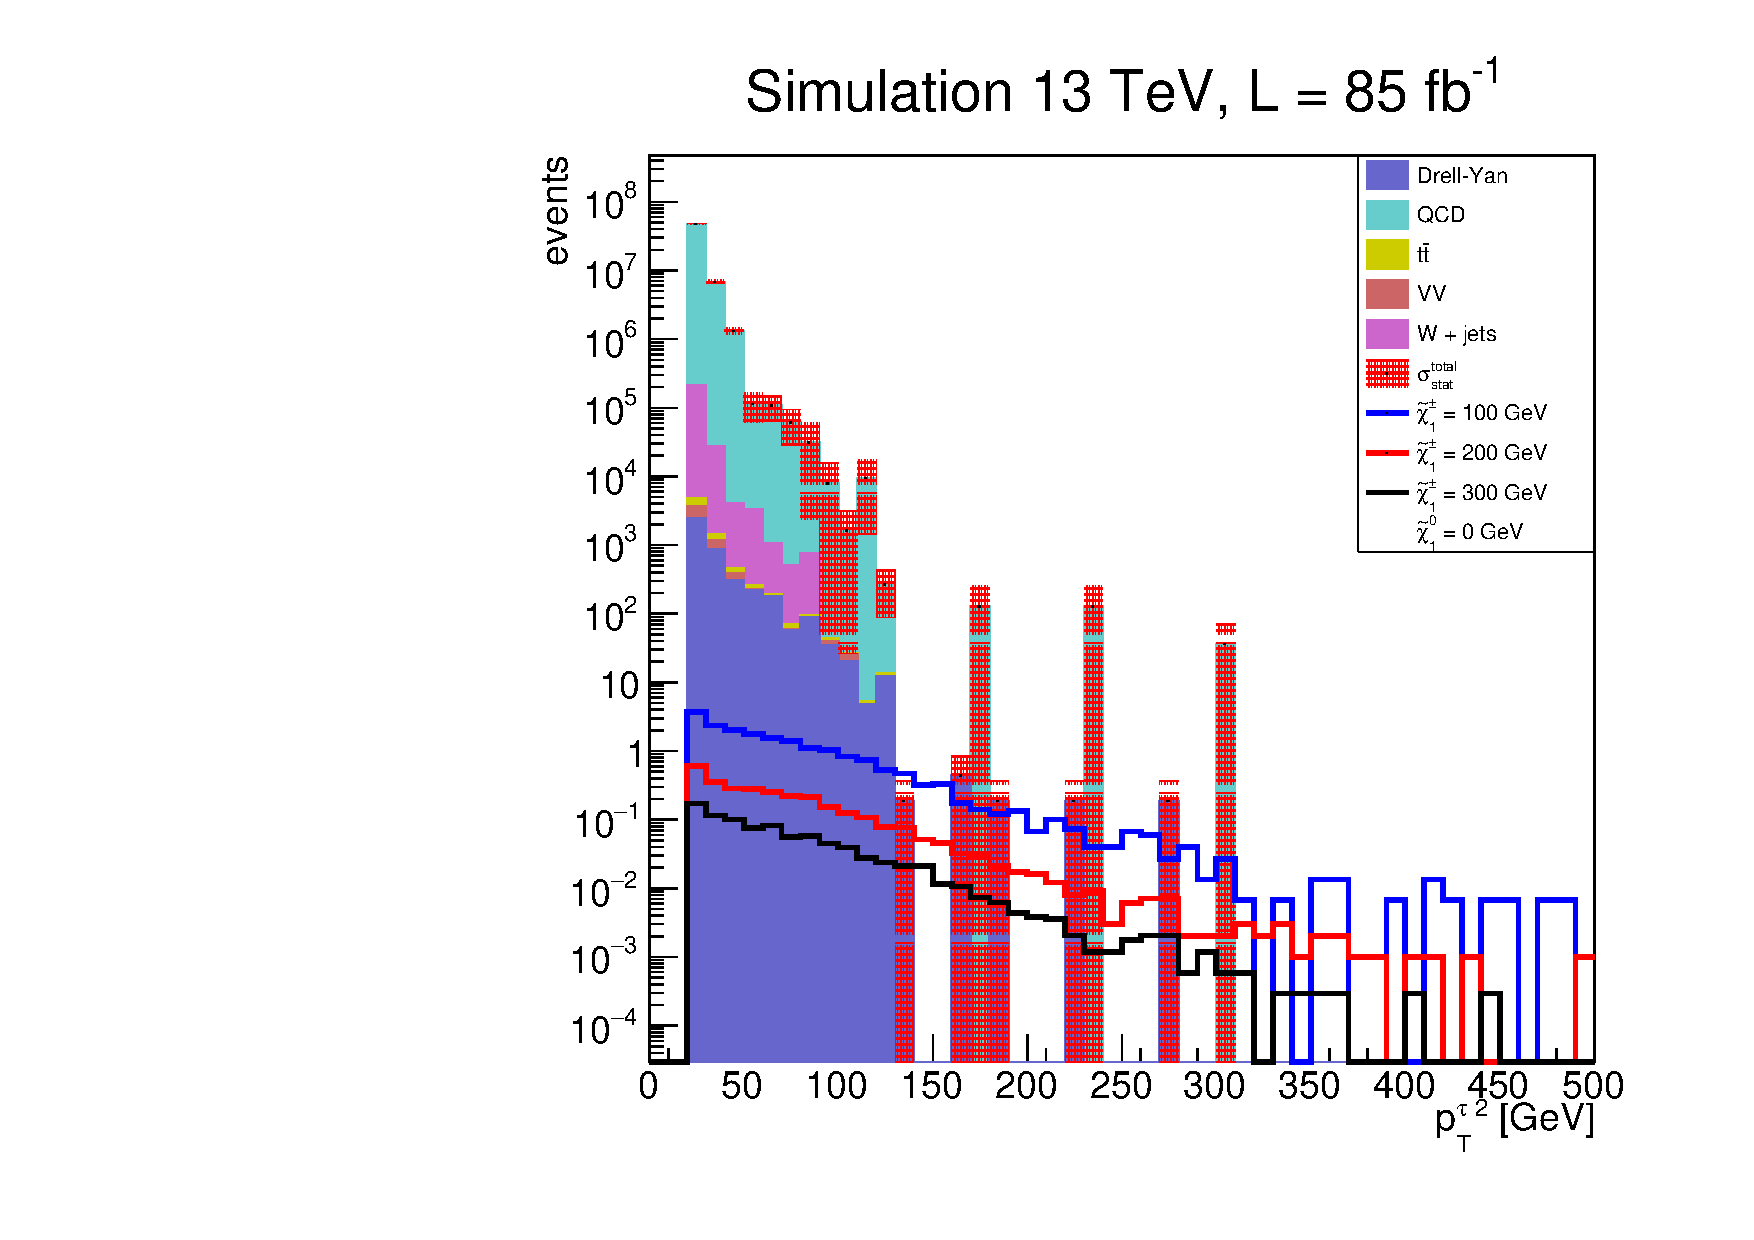
\includegraphics[width=0.5\textwidth]{analysis/pics/h_tau2pt_Tau2LooseIsoInclusiveVBFInverted.pdf} 		
	\end{tabular}
	\caption{(Left) Leading jet \pt distribution and (Right) and second leading \hadtau \pt distribution of selected signal and all MC background samples in control region 4.}
	\label{fig::crplots2_Tau2LooseIsoInclusiveVBFInverted_13tev}
\end{figure}

\clearpage

\section{Signal cross-section limits at 13 TeV}

This section shows the final results for the sensitivity study done on 13\tev simulated samples as function of the invariant mass of the di-jet candidate,  \met and the reconstructed \hadtau \pt. The different benchmark points were choses in term of \charginopm and \neutralinoone masses. As additional constraints the mass of \neutralinotwo is set as equal to \charginopm and mass difference between \stau and \charginopm is set to 5\gev.

\subsection*{\charginopm = \neutralinotwo = 100 GeV, \neutralinoone = 0 GeV}

\FloatBarrier

\begin{table}
	\begin{center}
		
		
		\begin{tabular}{| c | c | c | c | }
			\toprule
			\multicolumn{4}{| c | }{m(\charginopm) = m(\neutralinotwo) = 100\gev; m(\neutralinoone) = 0\gev} \\
			\midrule
			$\sigma_{lim}^{min}\pm(stat.)\pm(MC syst.)$ [pb]  & \pt(\hadtau) [GeV] & \mjj [GeV] & \met [GeV] \\
			\midrule
			$0.0327396\pm0.00680598^{+0.00312489}_{-0.00368623}$ & $<$ 20 & $<$ 250  & $<$ 130 \\			
			$0.0396705\pm0.00624294^{+0.0029859}_{-0.00362488}$ & $<$ 25 & $<$ 500  & $<$ 110 \\
			$0.0422022\pm0.0067994^{+0.00321255}_{-0.00389515}$ & $<$ 30 & $<$ 500  & $<$ 110 \\
			$0.0428261\pm0.00734389^{+0.00347889}_{-0.00418689}$ & $<$ 35 & $<$ 437.5  & $<$ 110 \\
			$0.0435307\pm0.00844122^{+0.00392365}_{-0.00466264}$ & $<$ 40 & $<$ 375  & $<$ 110 \\
			$0.0438139\pm0.00996139^{+0.00453651}_{-0.00529375}$ & $<$ 45 & $<$ 250  & $<$ 120 \\			
			\bottomrule
		\end{tabular}\caption{Cross section limit minimum reached at the given cuts for $m_{jj}$, \met and an increasing \pt(\hadtau) for \charginopm = \neutralinotwo = 100 GeV, \neutralinoone = 0 GeV benchmark point.}
		\label{table::xseclimmin_chi100_lsp000}
	\end{center}
\end{table}

\begin{figure}[tbh!]
	\centering
	\begin{tabular}{cc}
		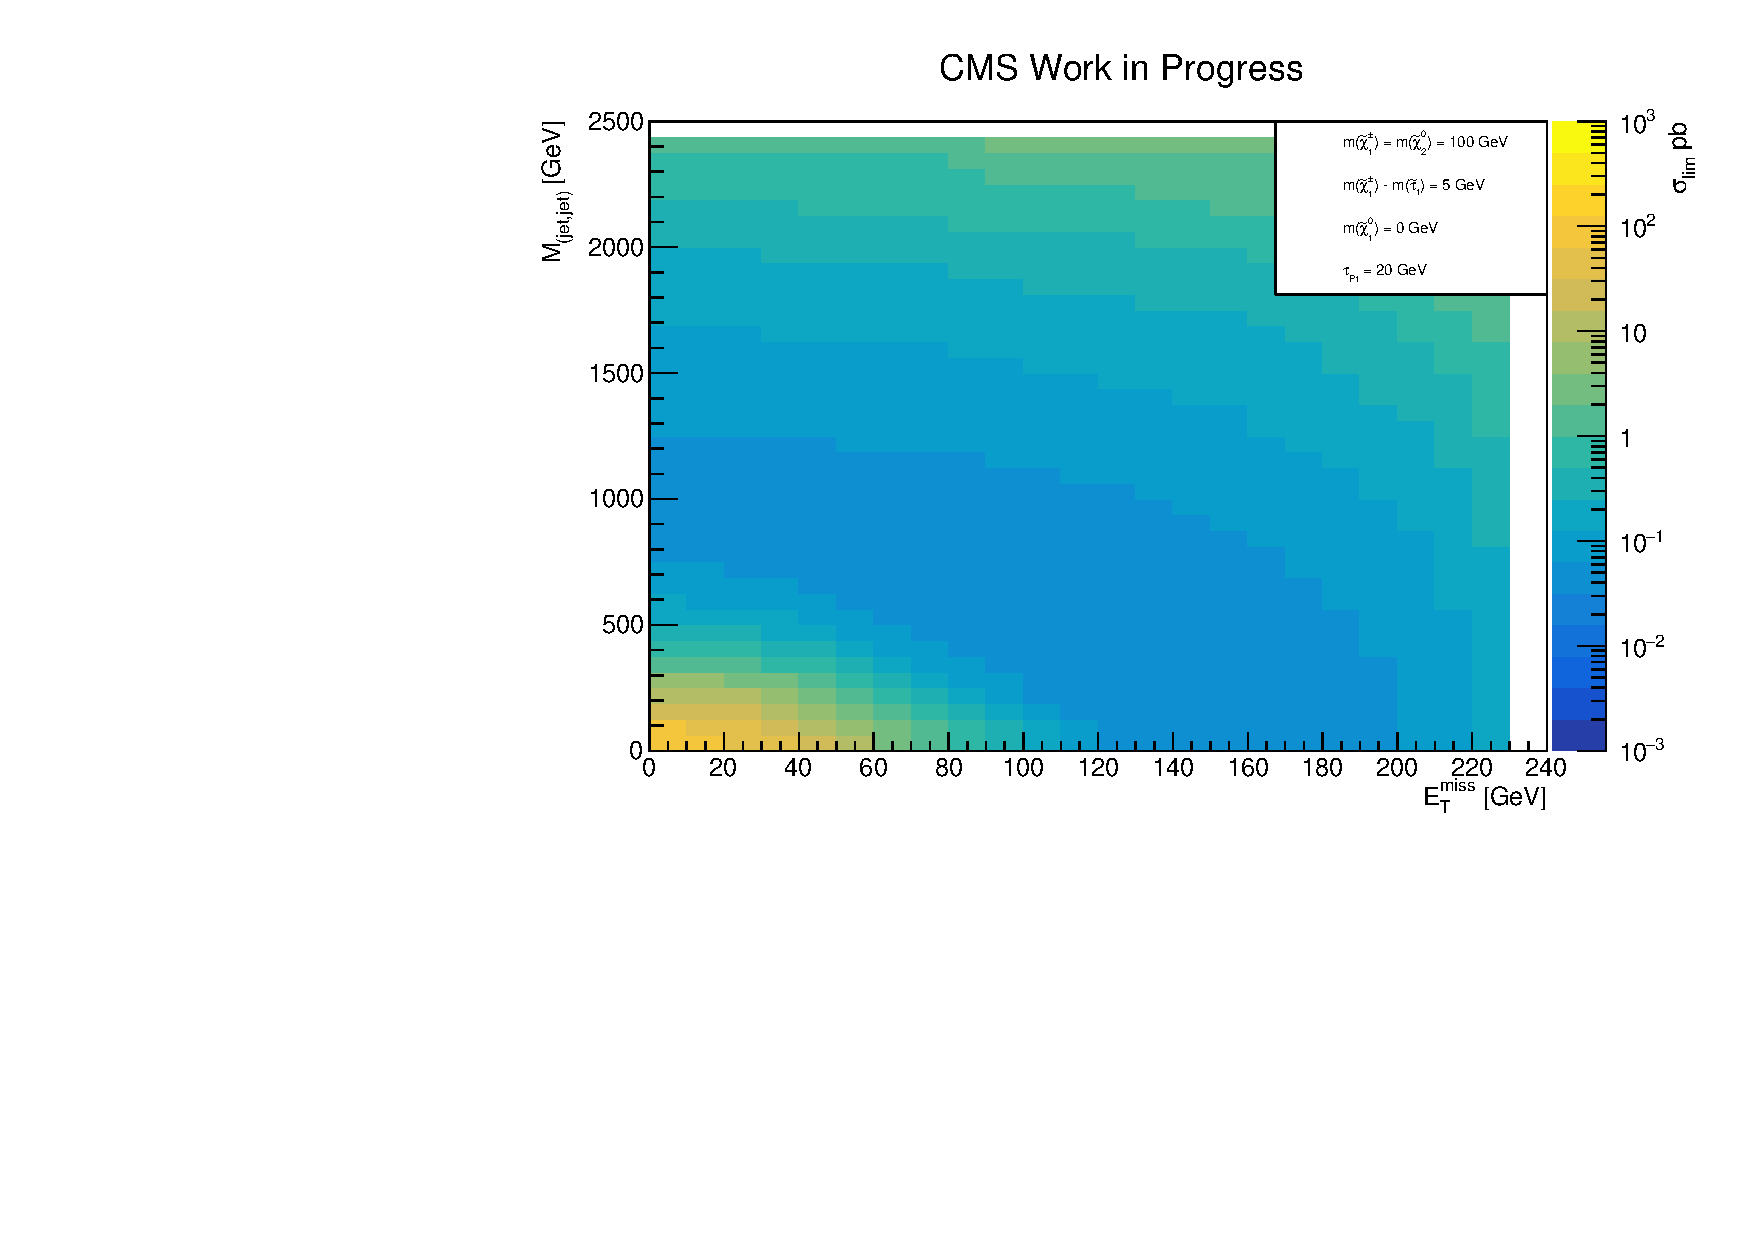
\includegraphics[width=0.45\textwidth]{analysis/pics/JetInvMass_vs_MET_xsec_chi100_lsp000_taupt20.pdf}
		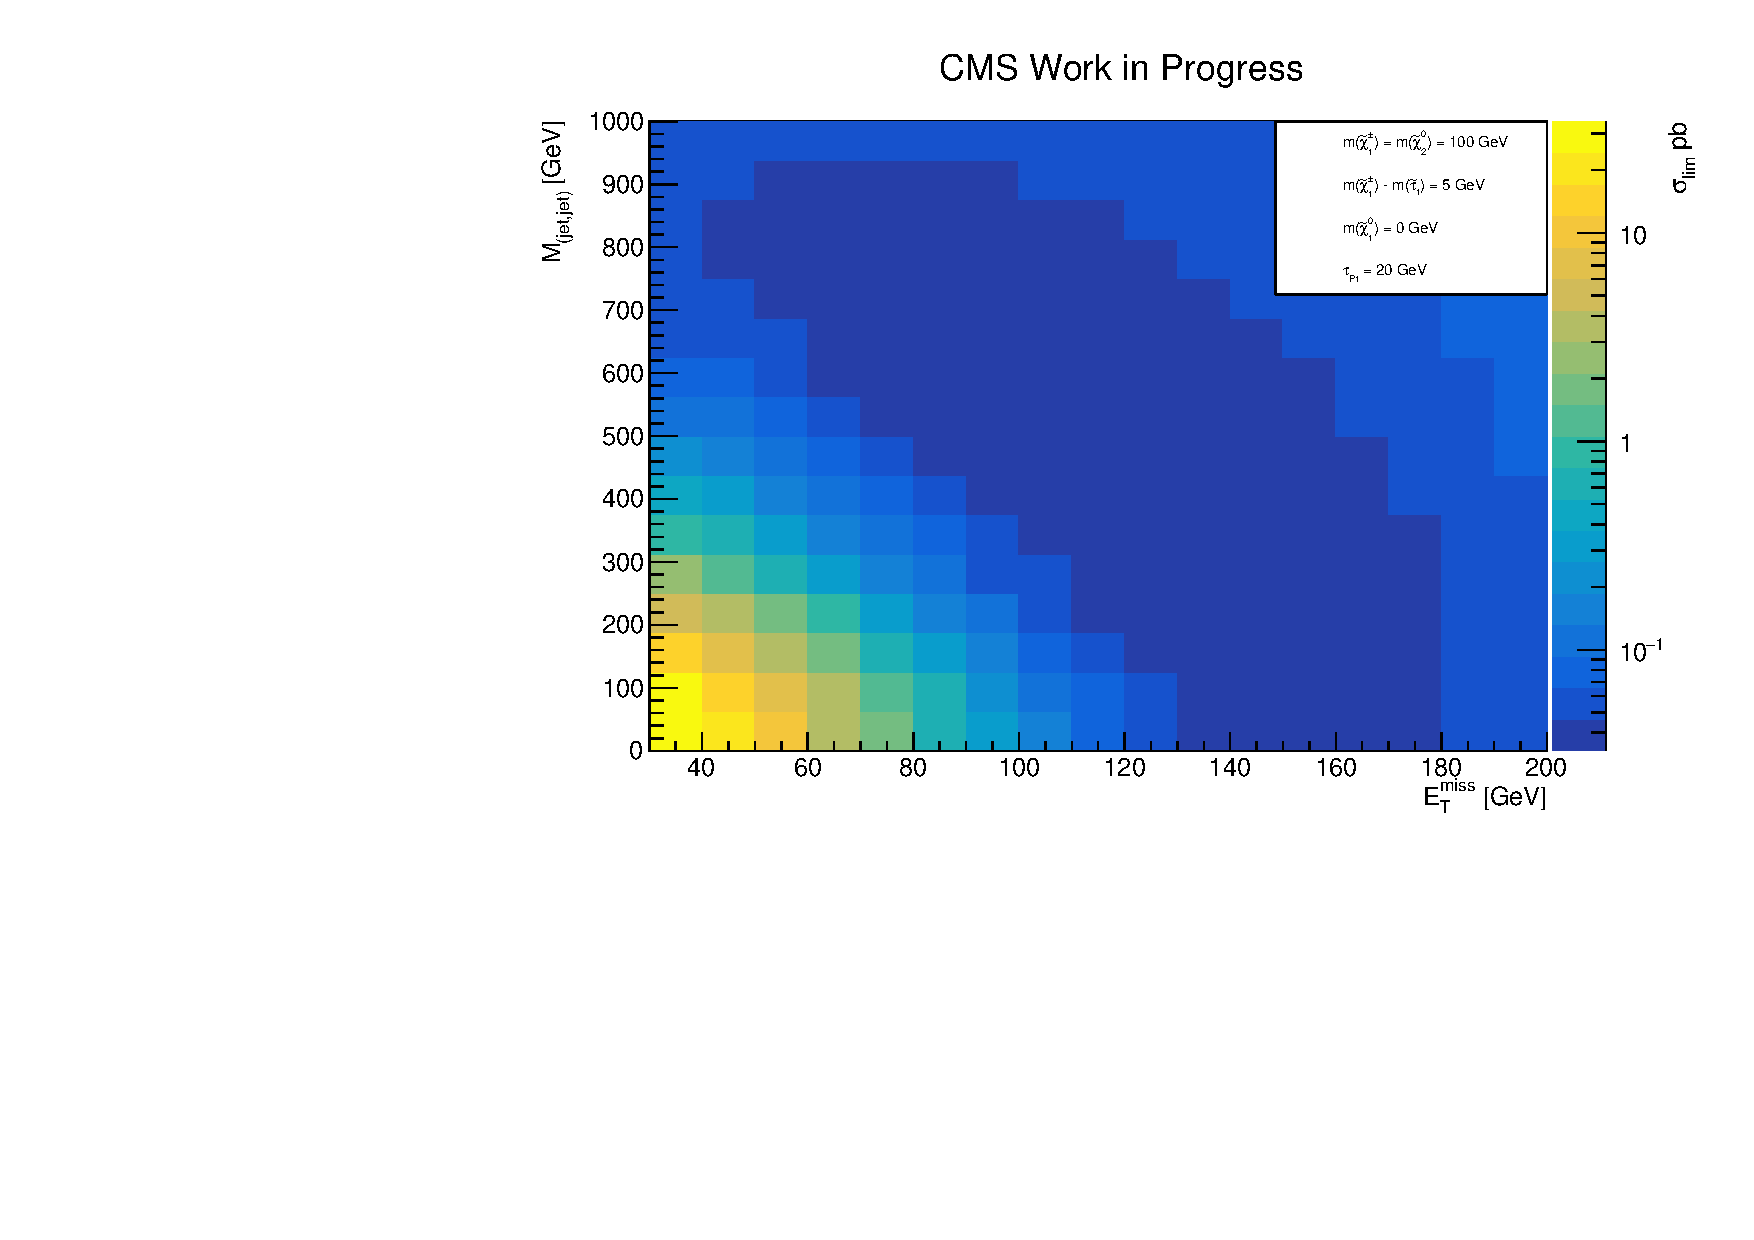
\includegraphics[width=0.45\textwidth]{analysis/pics/JetInvMass_vs_MET_xsec_chi100_lsp000_taupt20_zoom.pdf} 		
	\end{tabular}
	\caption{(Left) Cross section limit as function of $m_{jj}$ and \met for \charginopm = \neutralinotwo = 100 GeV, \neutralinoone = 0 GeV and an offline selection on $\pt(\hadtau) <  20\gev$. (Right) Zooming into the minimum cross section limit area for the same benchmark point.}
	\label{fig::JetInvMass_vs_MET_xsec_chi100_lsp000_taupt20}
\end{figure}

\begin{figure}[tbh!]
	\centering
	\begin{tabular}{cc}
		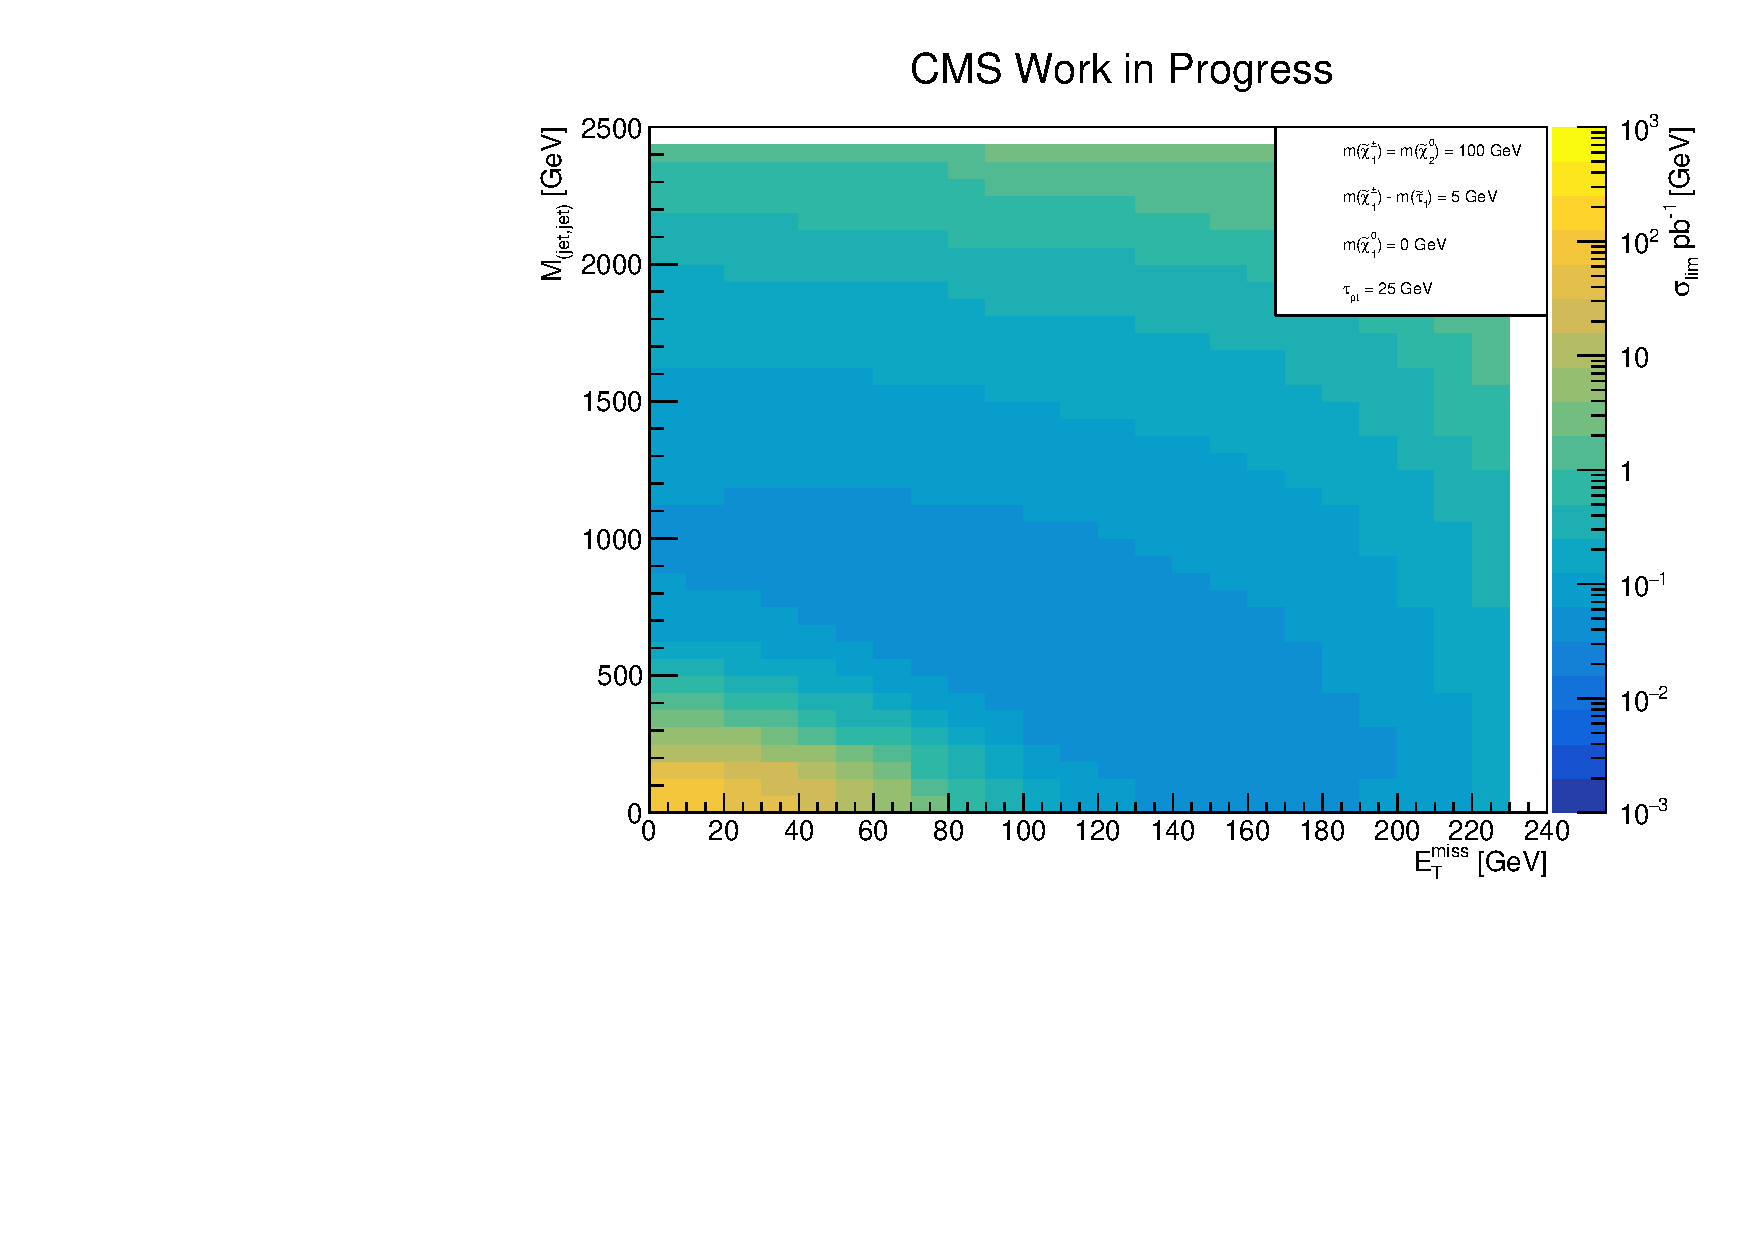
\includegraphics[width=0.45\textwidth]{analysis/pics/JetInvMass_vs_MET_xsec_chi100_lsp000_taupt25.pdf}
		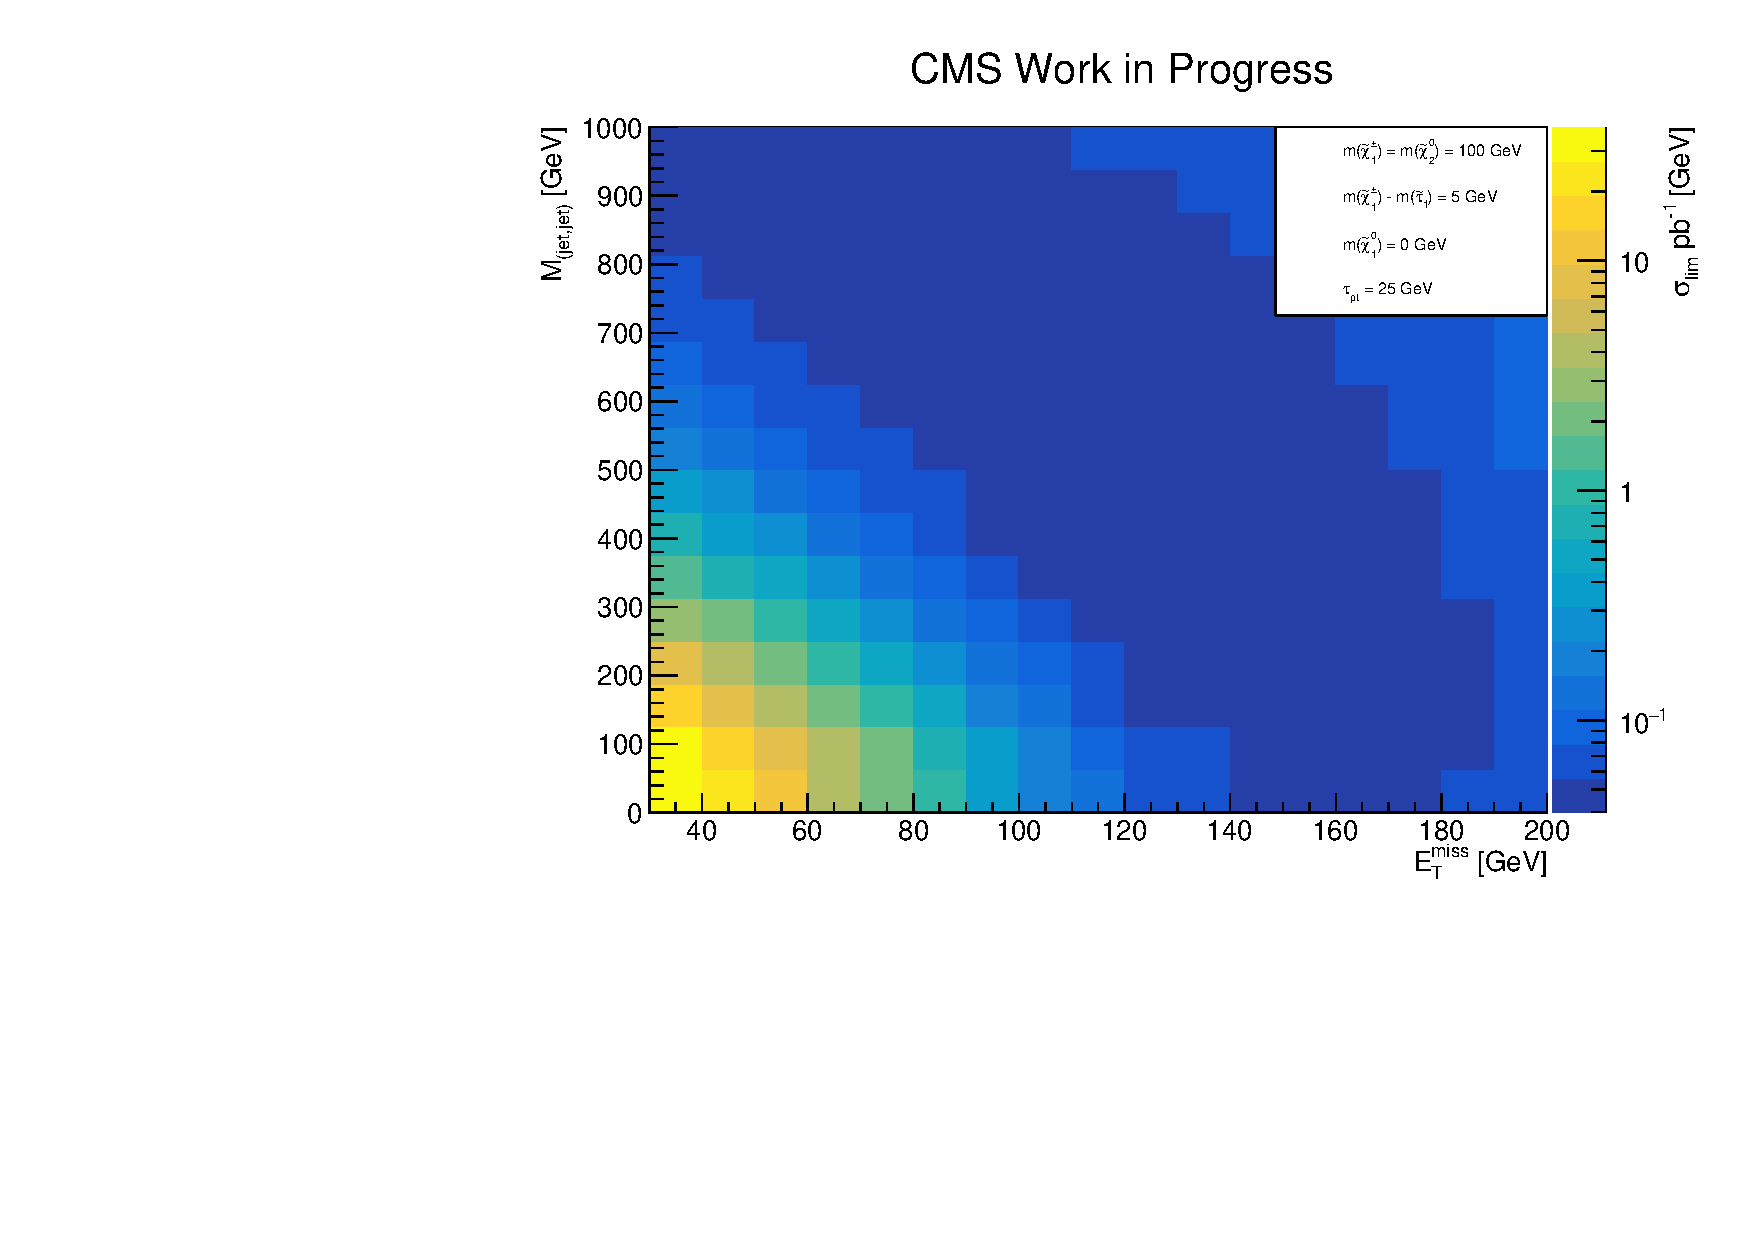
\includegraphics[width=0.45\textwidth]{analysis/pics/JetInvMass_vs_MET_xsec_chi100_lsp000_taupt25_zoom.pdf} 		
	\end{tabular}
	\caption{(Left) Cross section limit as function of $m_{jj}$ and \met for \charginopm = \neutralinotwo = 100 GeV, \neutralinoone = 0 GeV and an offline selection on $\pt(\hadtau) <  25\gev$. (Right) Zooming into the minimum cross section limit area for the same benchmark point.}
	\label{fig::JetInvMass_vs_MET_xsec_chi100_lsp000_taupt25}
\end{figure}

\begin{figure}[tbh!]
	\centering
	\begin{tabular}{cc}
		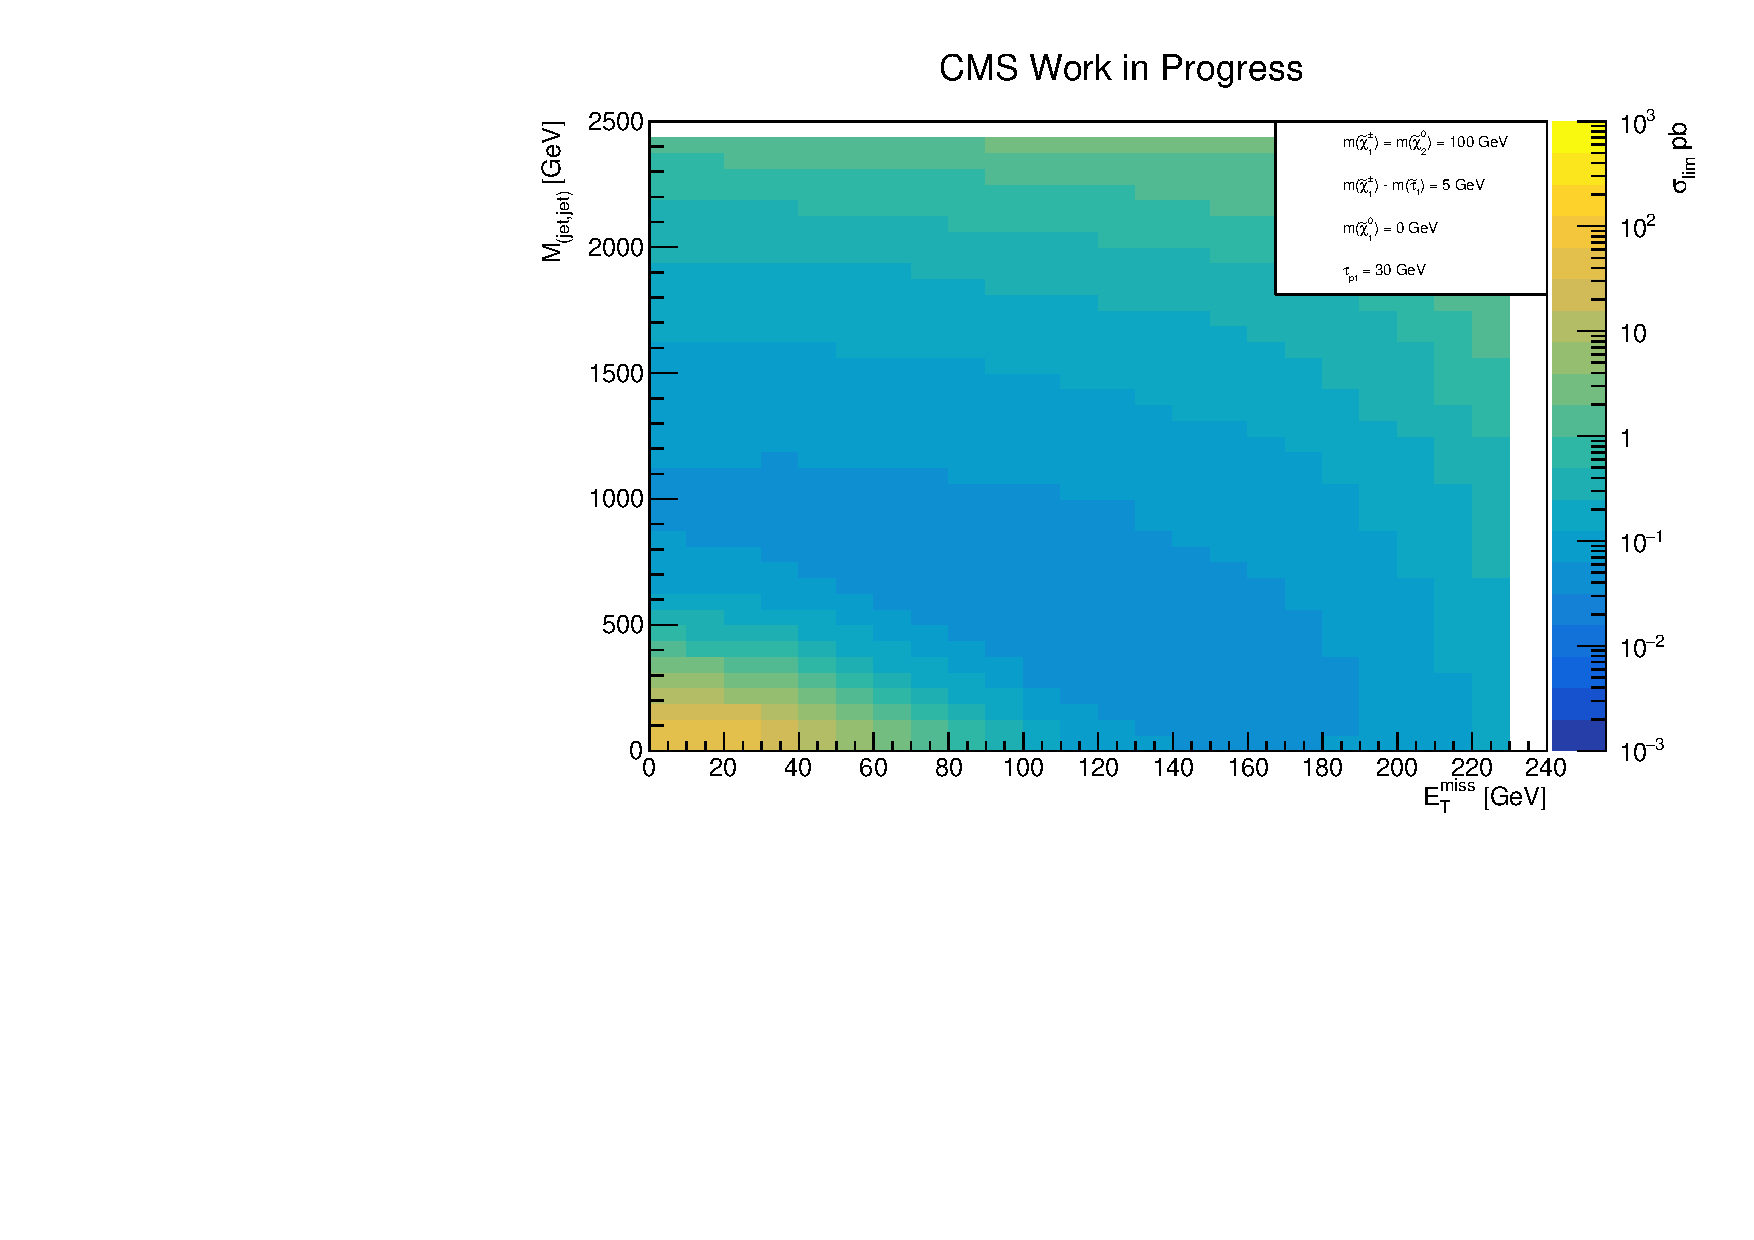
\includegraphics[width=0.45\textwidth]{analysis/pics/JetInvMass_vs_MET_xsec_chi100_lsp000_taupt30.pdf}
		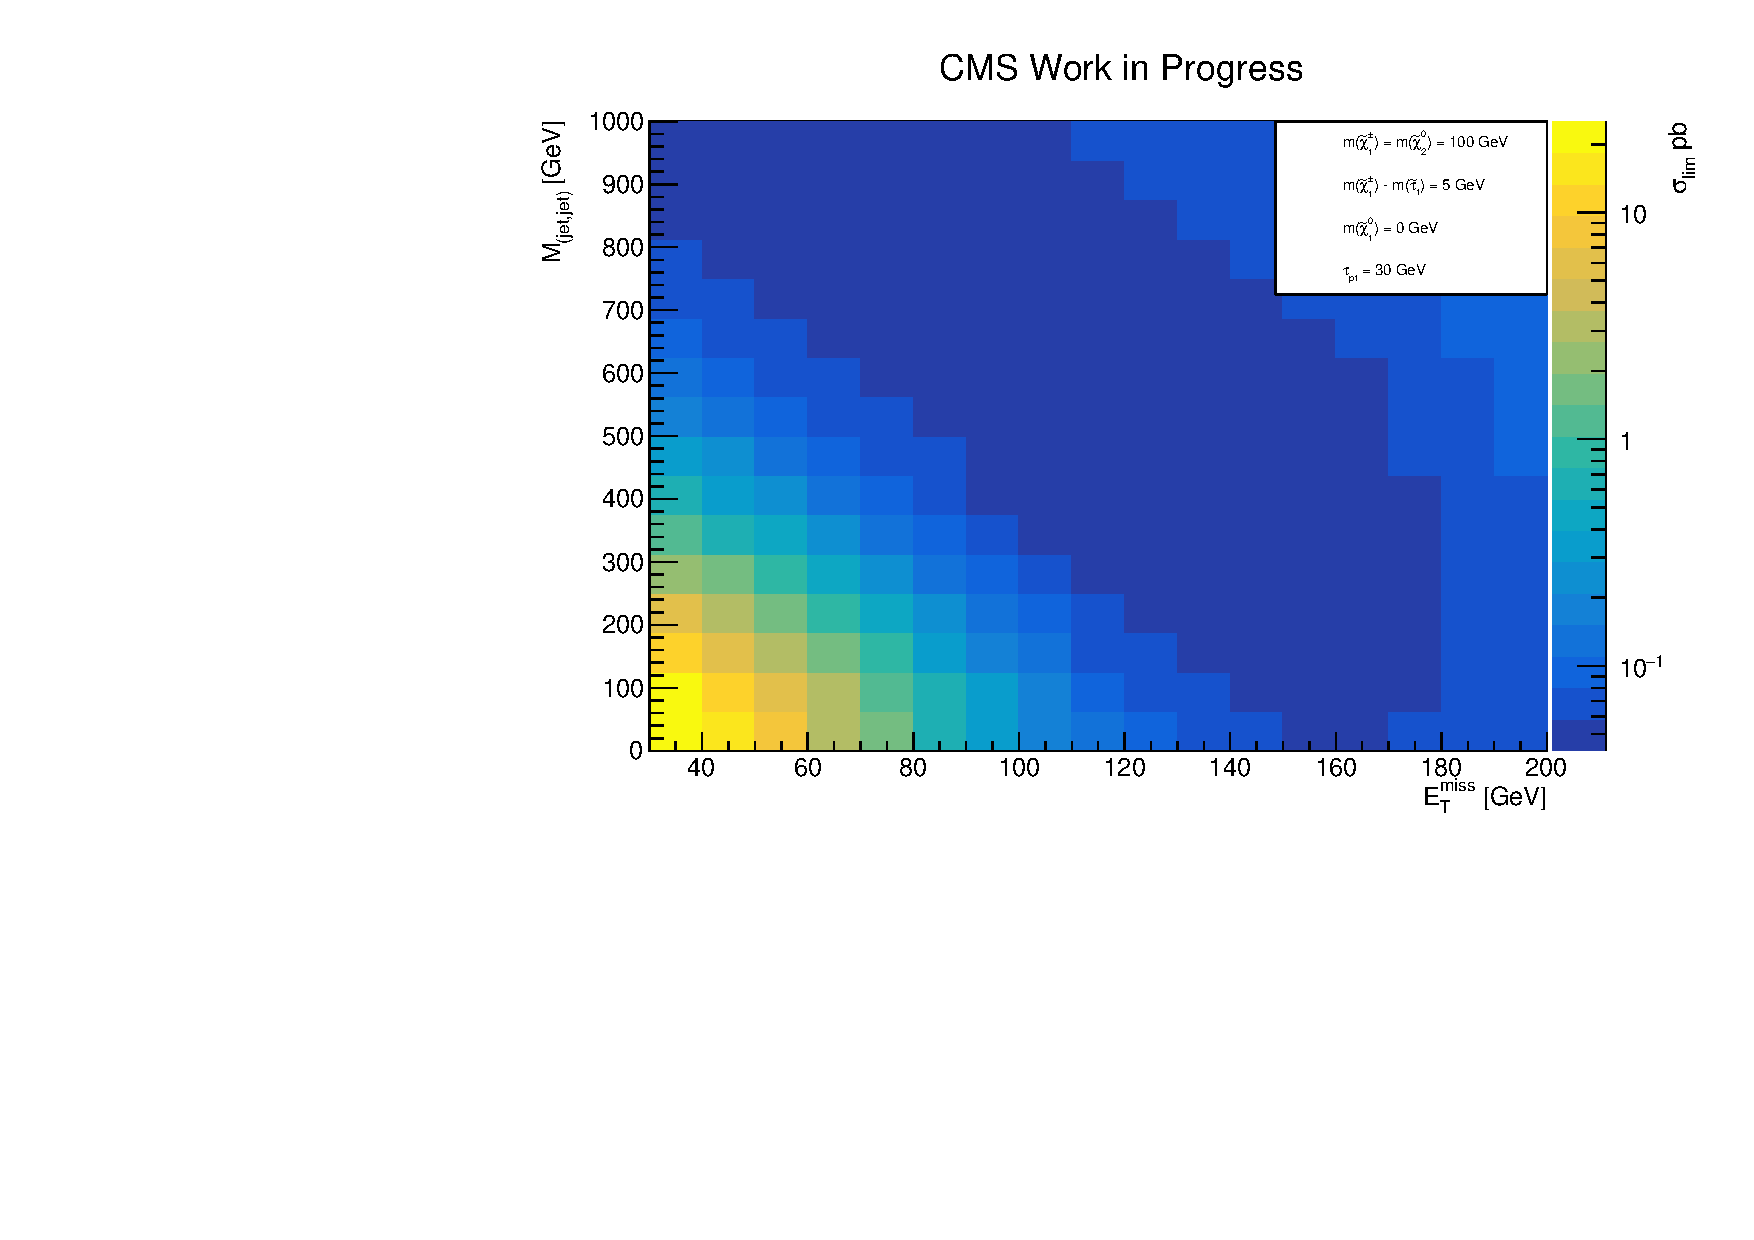
\includegraphics[width=0.45\textwidth]{analysis/pics/JetInvMass_vs_MET_xsec_chi100_lsp000_taupt30_zoom.pdf} 		
	\end{tabular}
	\caption{(Left) Cross section limit as function of $m_{jj}$ and \met for \charginopm = \neutralinotwo = 100 GeV, \neutralinoone = 0 GeV and an offline selection on $\pt(\hadtau) <  30\gev$. (Right) Zooming into the minimum cross section limit area for the same benchmark point.}
	\label{fig::JetInvMass_vs_MET_xsec_chi100_lsp000_taupt30}
\end{figure}

\begin{figure}[tbh!]
	\centering
	\begin{tabular}{cc}
		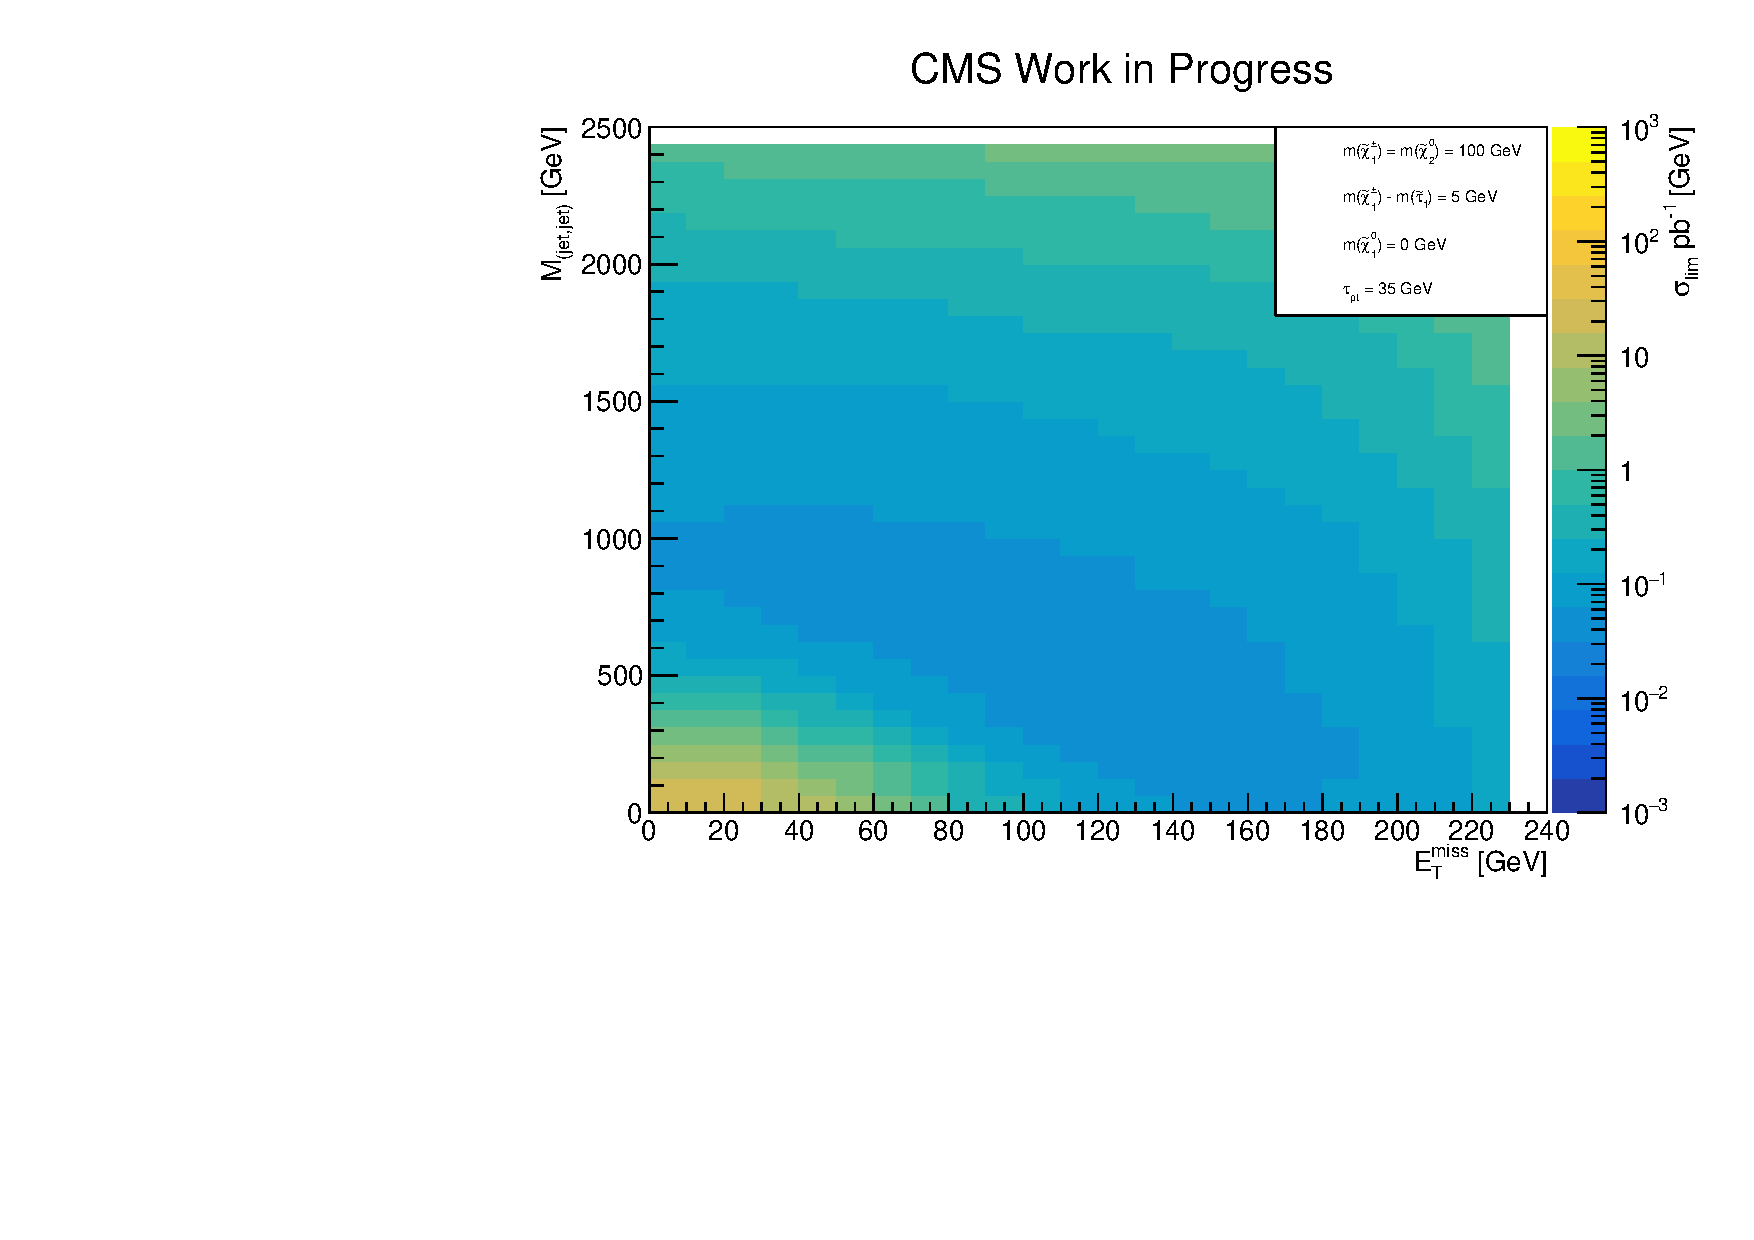
\includegraphics[width=0.45\textwidth]{analysis/pics/JetInvMass_vs_MET_xsec_chi100_lsp000_taupt35.pdf}
		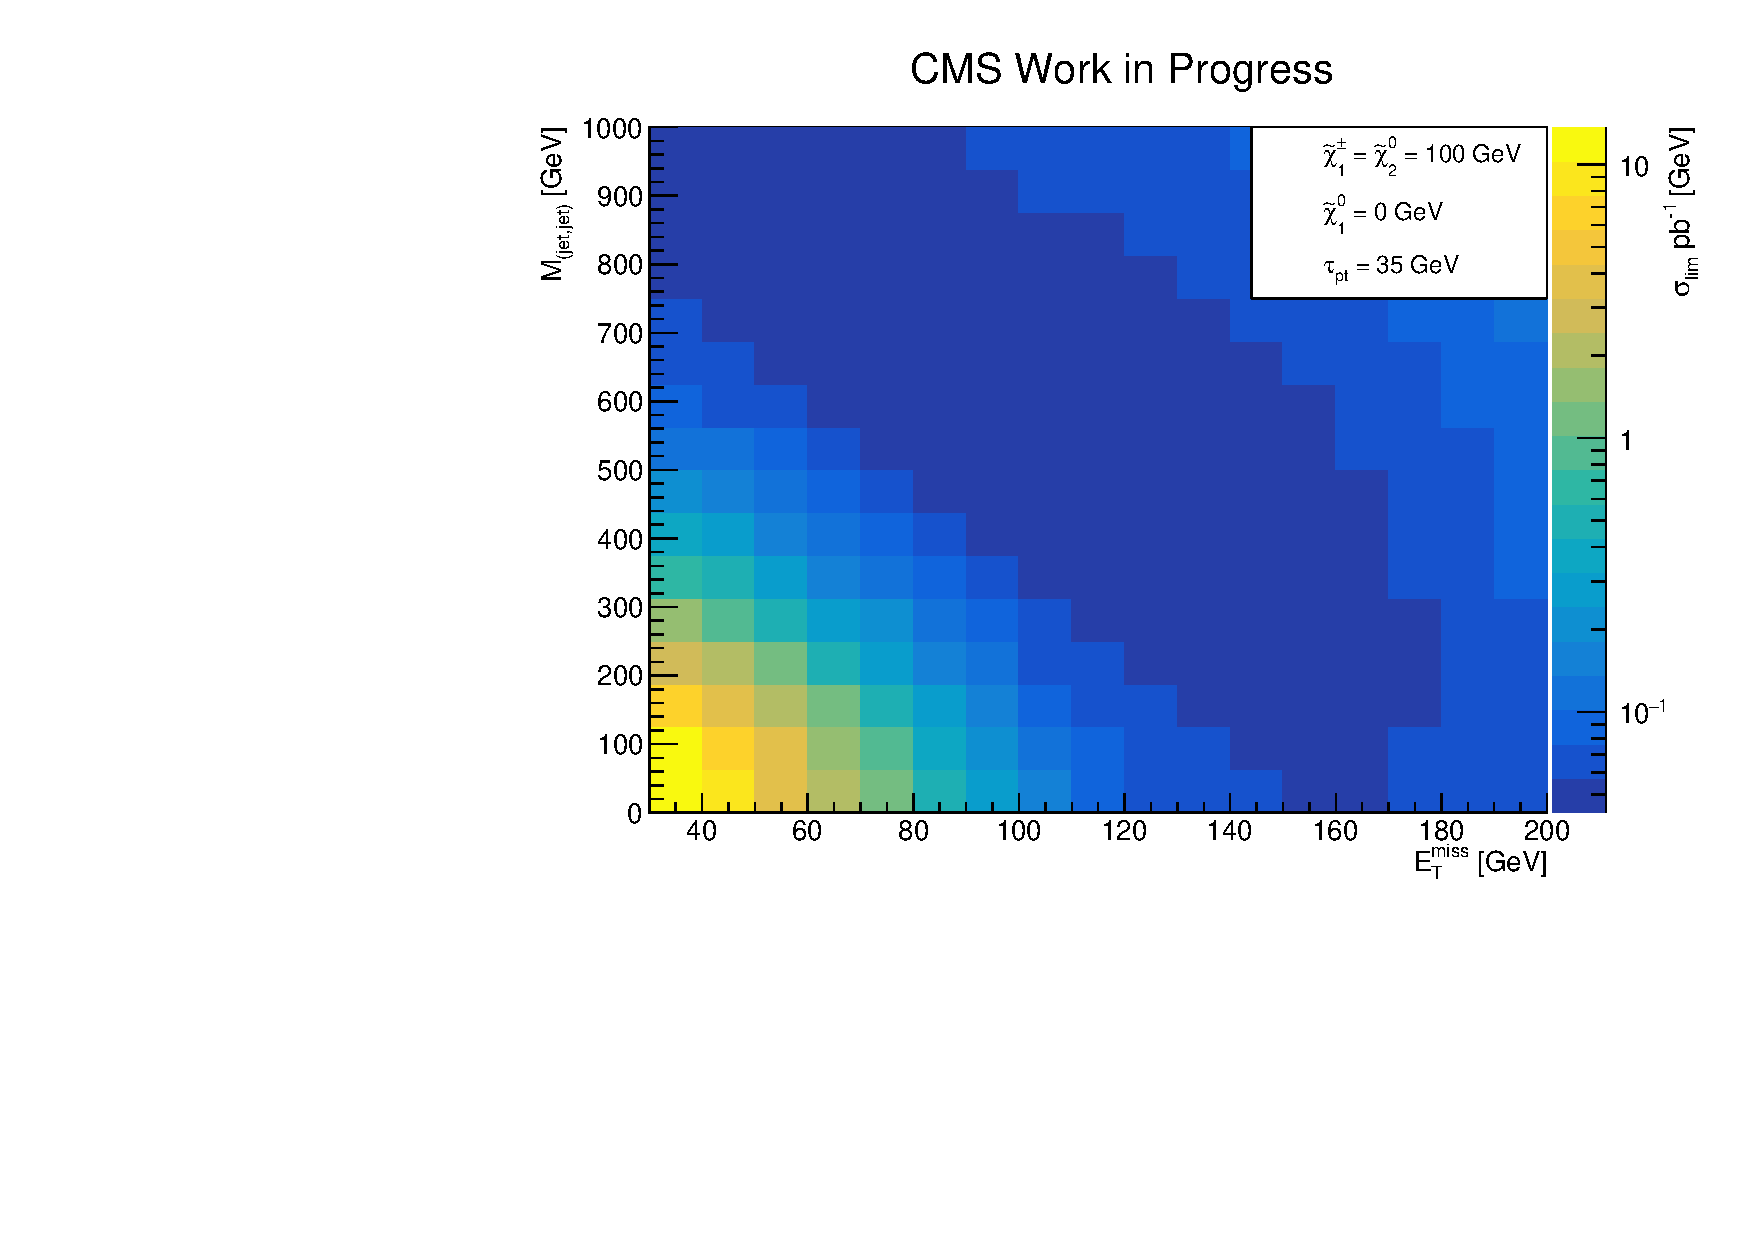
\includegraphics[width=0.45\textwidth]{analysis/pics/JetInvMass_vs_MET_xsec_chi100_lsp000_taupt35_zoom.pdf} 		
	\end{tabular}
	\caption{(Left) Cross section limit as function of $m_{jj}$ and \met for \charginopm = \neutralinotwo = 100 GeV, \neutralinoone = 0 GeV and an offline selection on $\pt(\hadtau) <  35\gev$. (Right) Zooming into the minimum cross section limit area for the same benchmark point.}
	\label{fig::JetInvMass_vs_MET_xsec_chi100_lsp000_taupt35}
\end{figure}

\begin{figure}[tbh!]
	\centering
	\begin{tabular}{cc}
		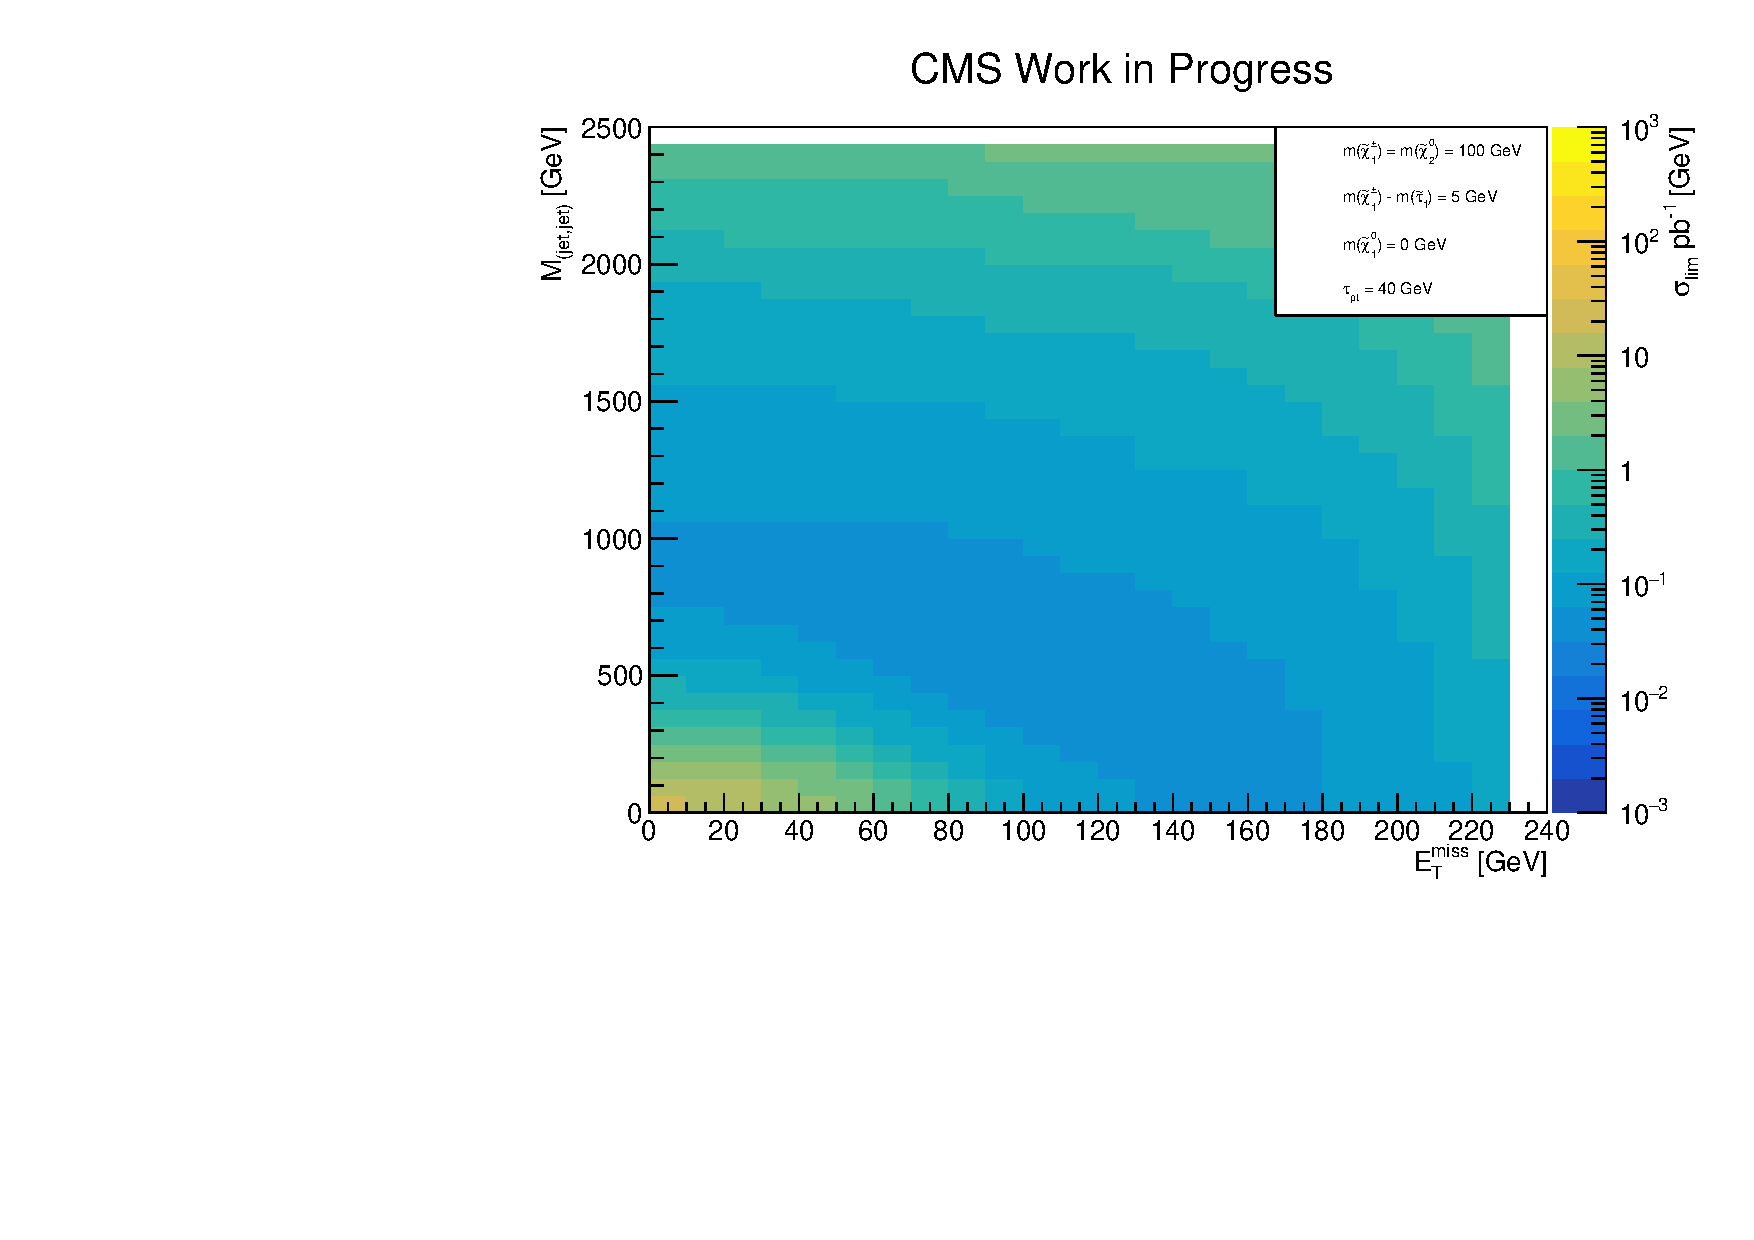
\includegraphics[width=0.45\textwidth]{analysis/pics/JetInvMass_vs_MET_xsec_chi100_lsp000_taupt40.pdf}
		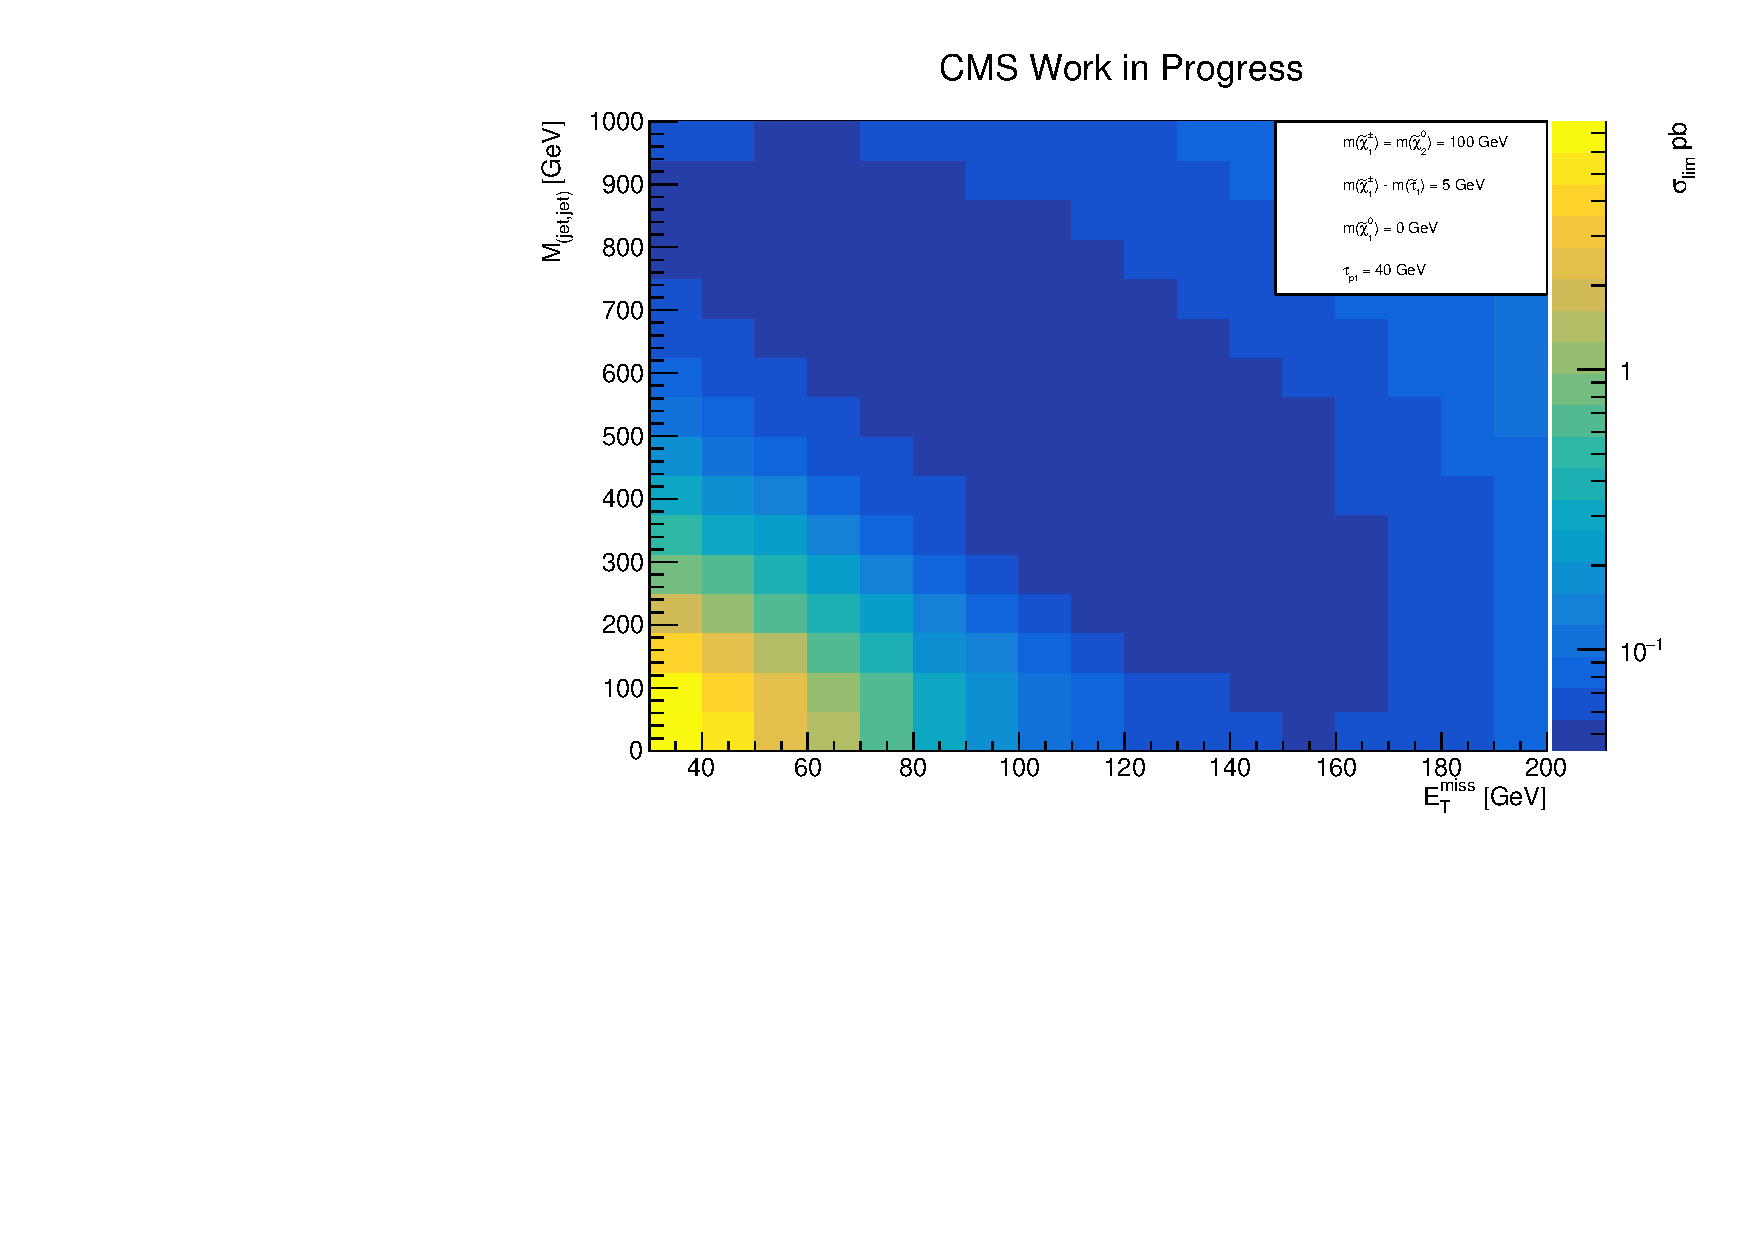
\includegraphics[width=0.45\textwidth]{analysis/pics/JetInvMass_vs_MET_xsec_chi100_lsp000_taupt40_zoom.pdf} 		
	\end{tabular}
	\caption{(Left) Cross section limit as function of $m_{jj}$ and \met for \charginopm = \neutralinotwo = 100 GeV, \neutralinoone = 0 GeV and an offline selection on $\pt(\hadtau) <  40\gev$. (Right) Zooming into the minimum cross section limit area for the same benchmark point.}
	\label{fig::JetInvMass_vs_MET_xsec_chi100_lsp000_taupt40}
\end{figure}

\begin{figure}[tbh!]
	\centering
	\begin{tabular}{cc}
		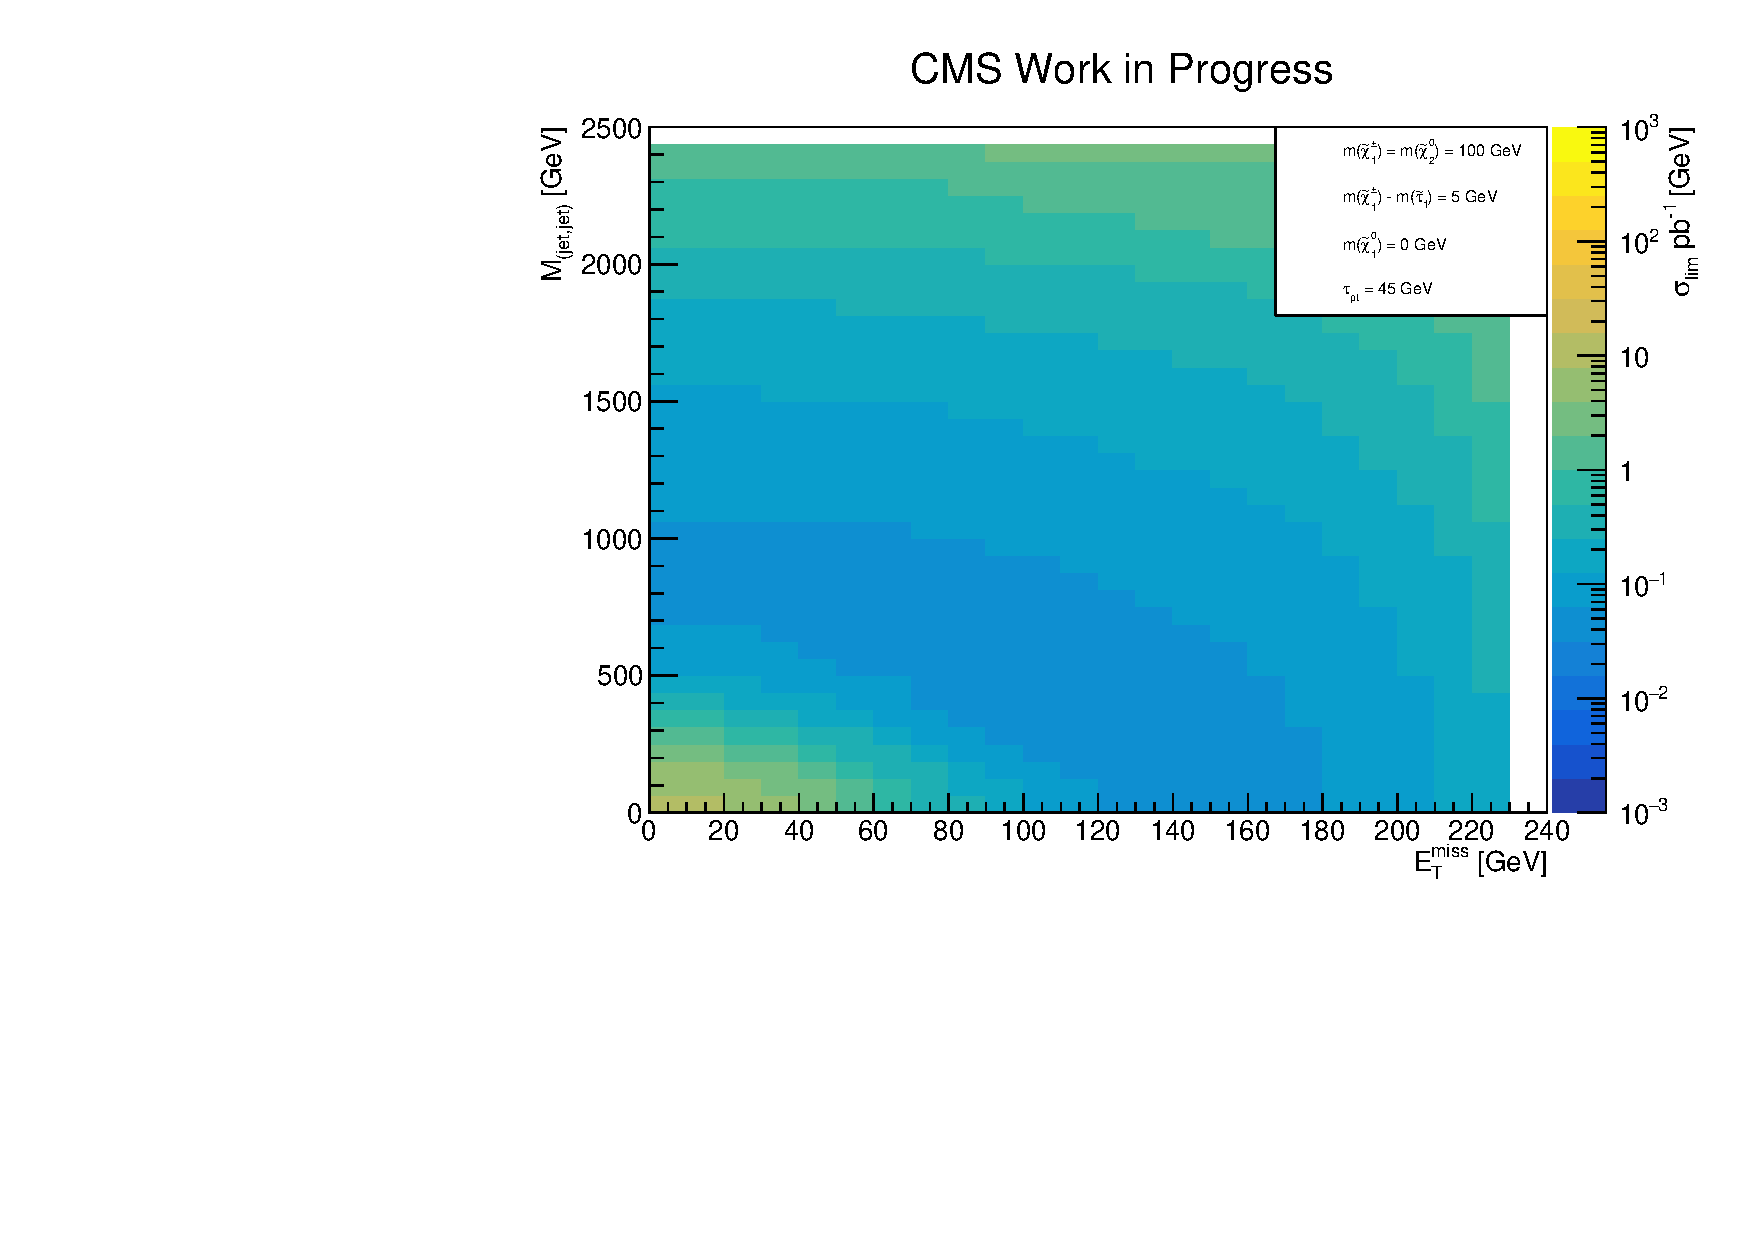
\includegraphics[width=0.45\textwidth]{analysis/pics/JetInvMass_vs_MET_xsec_chi100_lsp000_taupt45.pdf}
		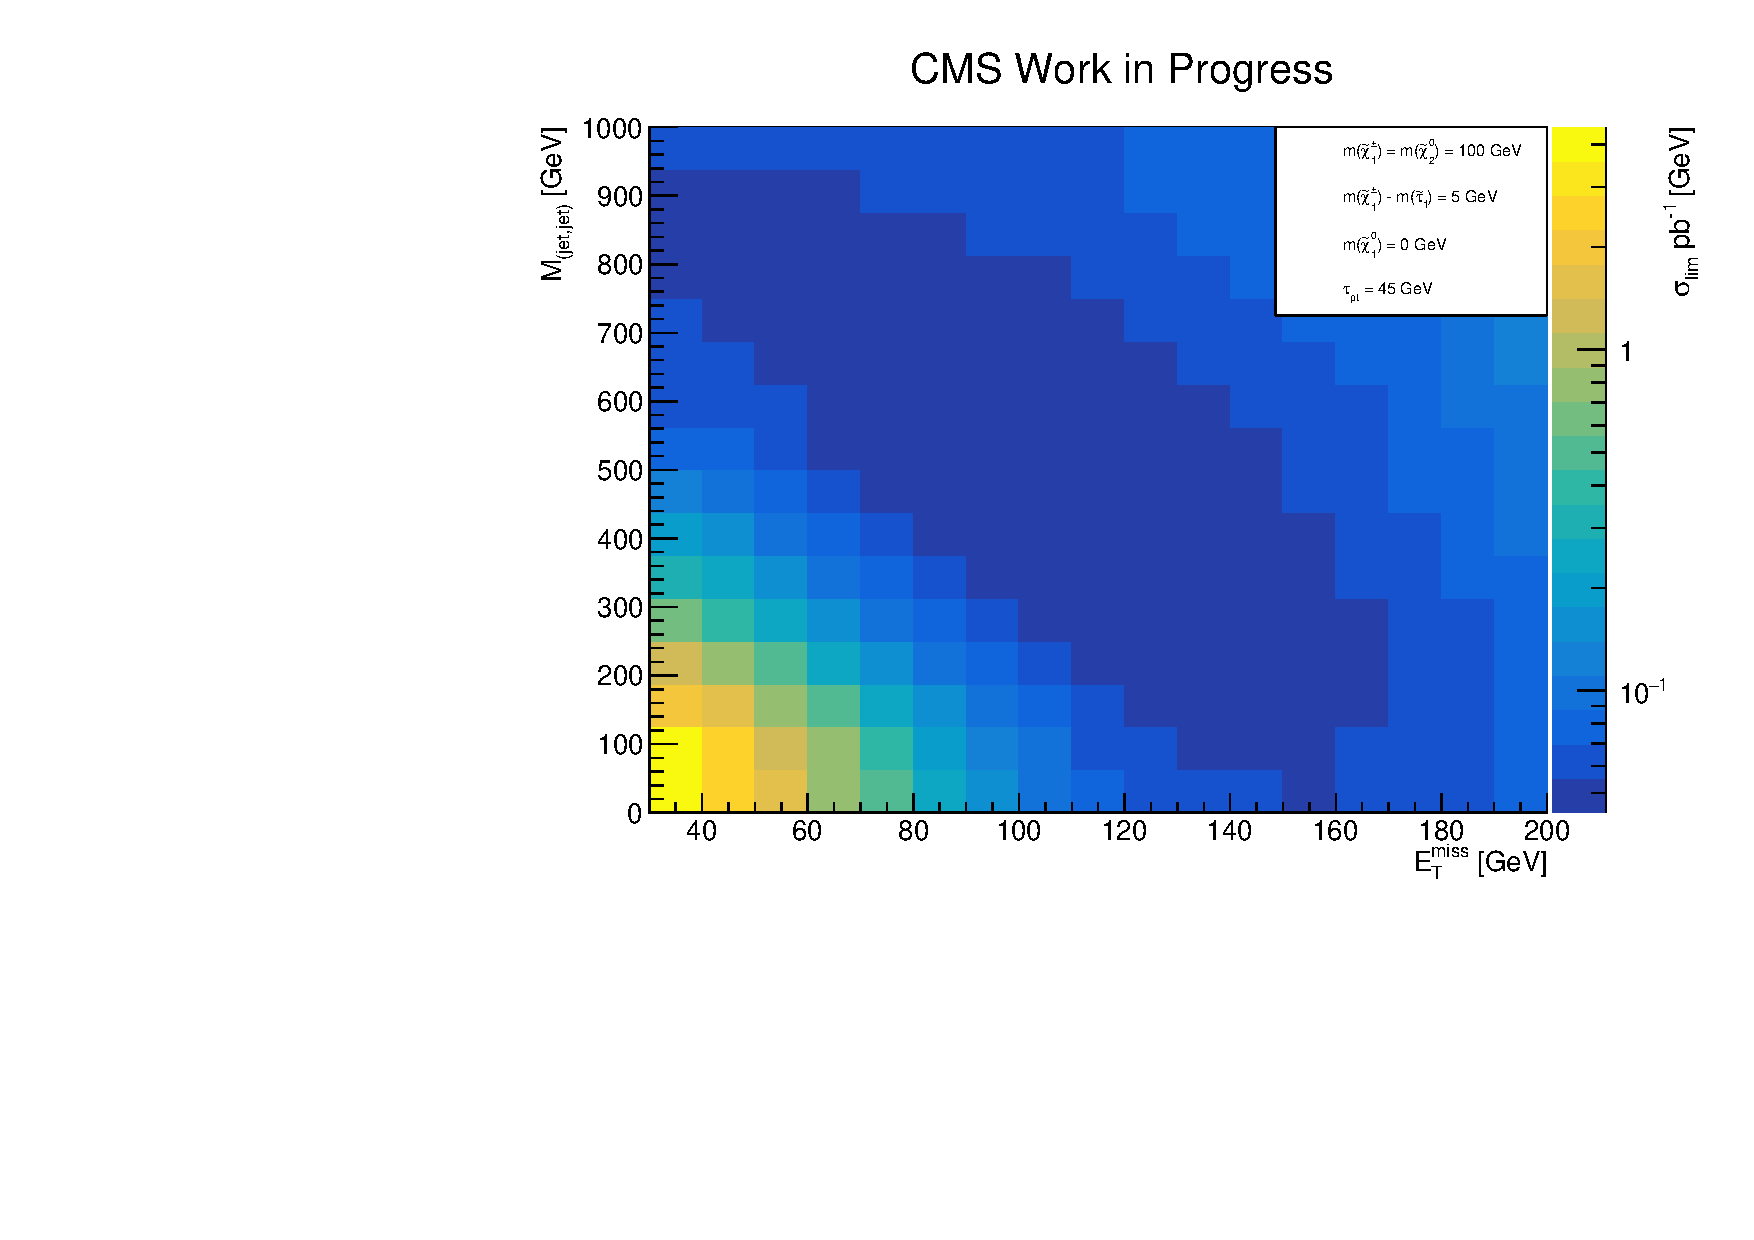
\includegraphics[width=0.45\textwidth]{analysis/pics/JetInvMass_vs_MET_xsec_chi100_lsp000_taupt45_zoom.pdf} 		
	\end{tabular}
	\caption{(Left) Cross section limit as function of $m_{jj}$ and \met for \charginopm = \neutralinotwo = 100 GeV, \neutralinoone = 0 GeV and an offline selection on $\pt(\hadtau) <  45\gev$. (Right) Zooming into the minimum cross section limit area for the same benchmark point.}
	\label{fig::JetInvMass_vs_MET_xsec_chi100_lsp000_taupt45}
\end{figure}

\FloatBarrier

\subsection*{\charginopm = \neutralinotwo = 200 GeV, \neutralinoone = 0 GeV}

\FloatBarrier

\begin{table}
	\begin{center}
		\begin{tabular}{| c | c | c | c | }
			\toprule
			\multicolumn{4}{| c | }{m(\charginopm) = m(\neutralinotwo) = 200\gev; m(\neutralinoone) = 0\gev} \\
			\midrule
			$\sigma_{lim}^{min}\pm(stat.)\pm(MC syst.)$ [pb]  & \pt(\hadtau) [GeV] & \mjj [GeV] & \met [GeV] \\
			\midrule
			$0.0333074\pm0.0069229^{+0.00317908}_{-0.00375015}$& $<$ 20 & $<$ 250  & $<$ 130 \\			
			$0.0333074\pm0.0069229^{+0.00317908}_{-0.00375015}$ & $<$ 20 & $<$ 250  & $<$ 130 \\			
			$0.0417626\pm0.00933586^{+0.00419533}_{-0.00491559}$ & $<$ 30 & $<$ 312.5  & $<$ 130 \\			
			$0.0415464\pm0.0100895^{+0.00450281}_{-0.00522173}$ & $<$ 35 & $<$ 312.5  & $<$ 120 \\			
			$0.0415724\pm0.00805613^{+0.00374942}_{-0.00445526}$ & $<$ 40 & $<$ 312.5  & $<$ 120 \\			
			$0.0428067\pm0.00707501^{+0.0033864}_{-0.00408814}$ & $<$ 45 & $<$ 312.5  & $<$ 120 \\
			\bottomrule
		\end{tabular}\caption{Cross section limit minimum reached at the given cuts for $m_{jj}$, \met and an increasing \pt(\hadtau) for \charginopm = \neutralinotwo = 200 GeV, \neutralinoone = 0 GeV benchmark point.}
		\label{table::xseclimmin_chi200_lsp000}
	\end{center}
\end{table}

\begin{figure}[tbh!]
	\centering
	\begin{tabular}{cc}
		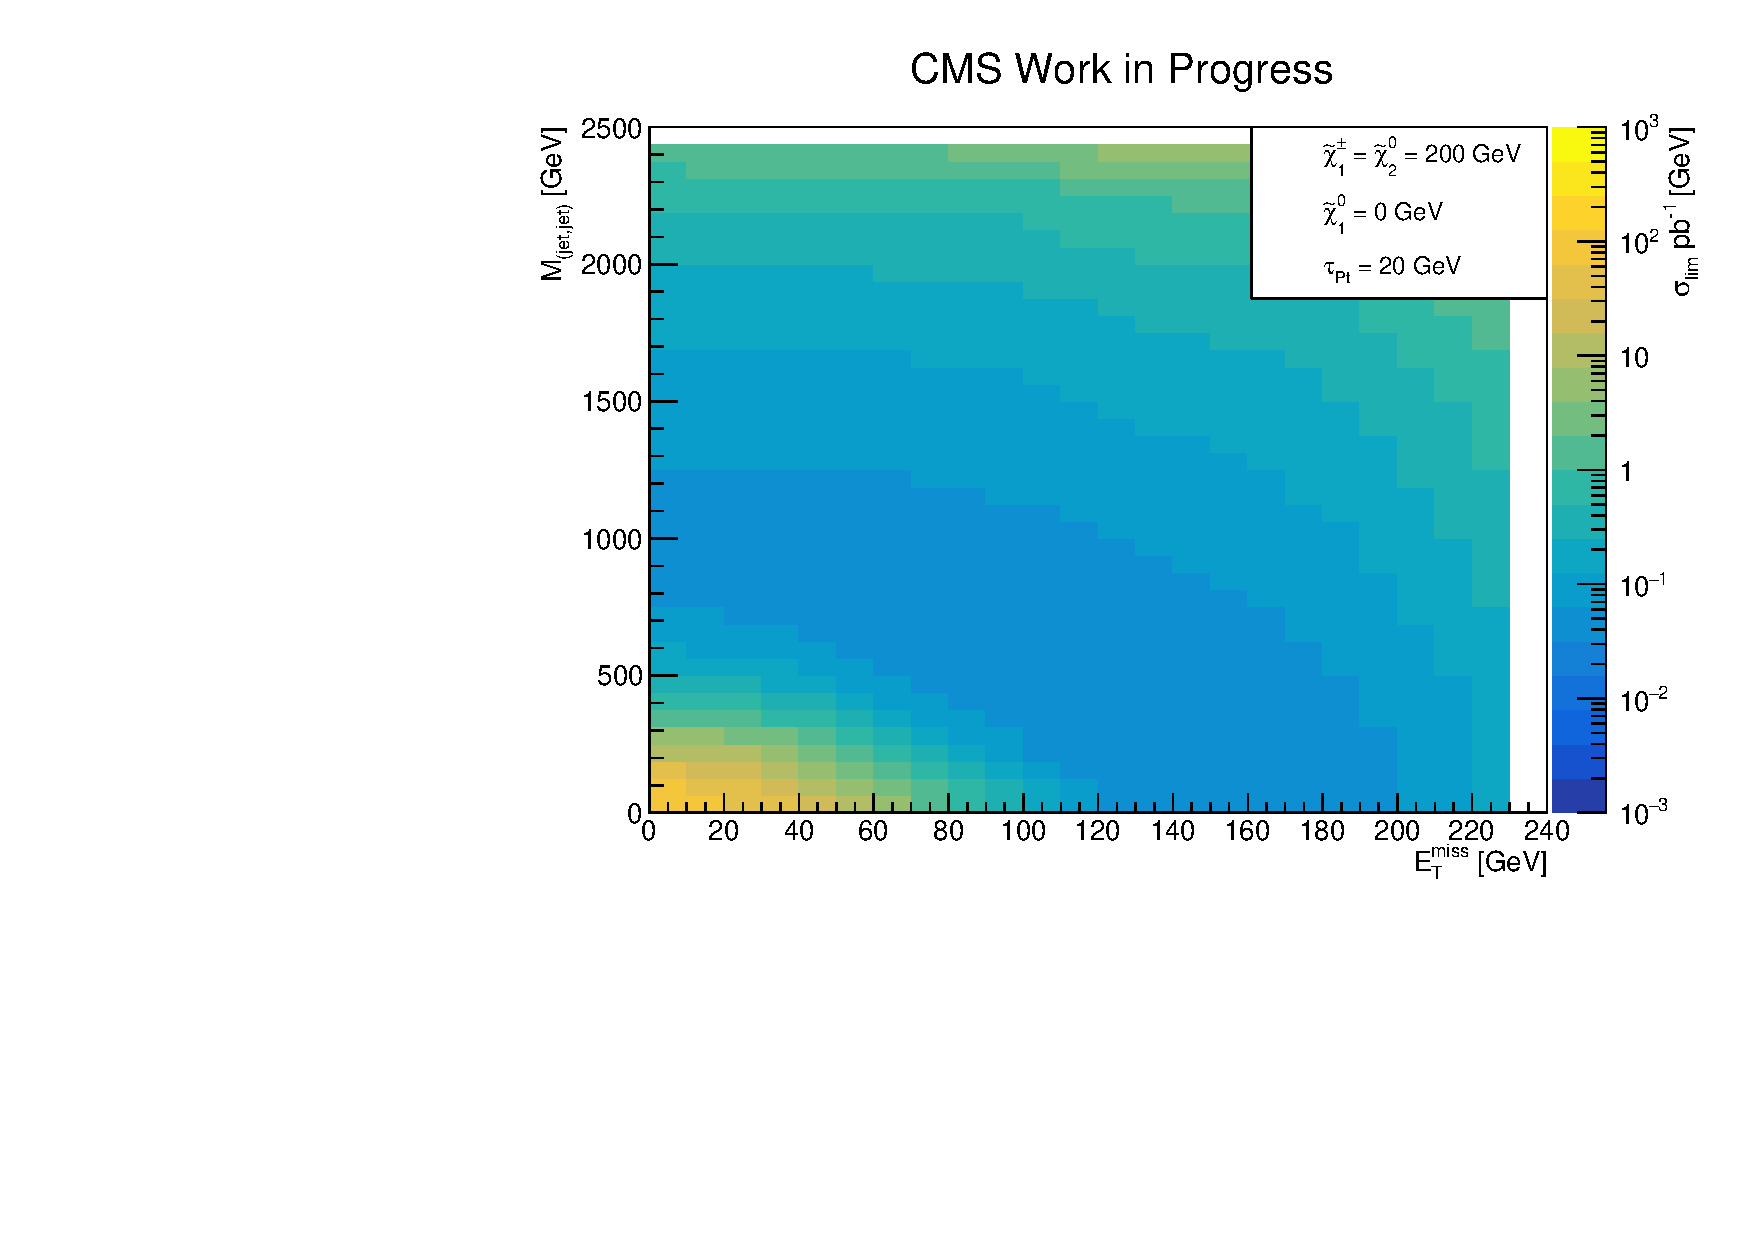
\includegraphics[width=0.45\textwidth]{analysis/pics/JetInvMass_vs_MET_xsec_chi200_lsp000_taupt20.pdf}
		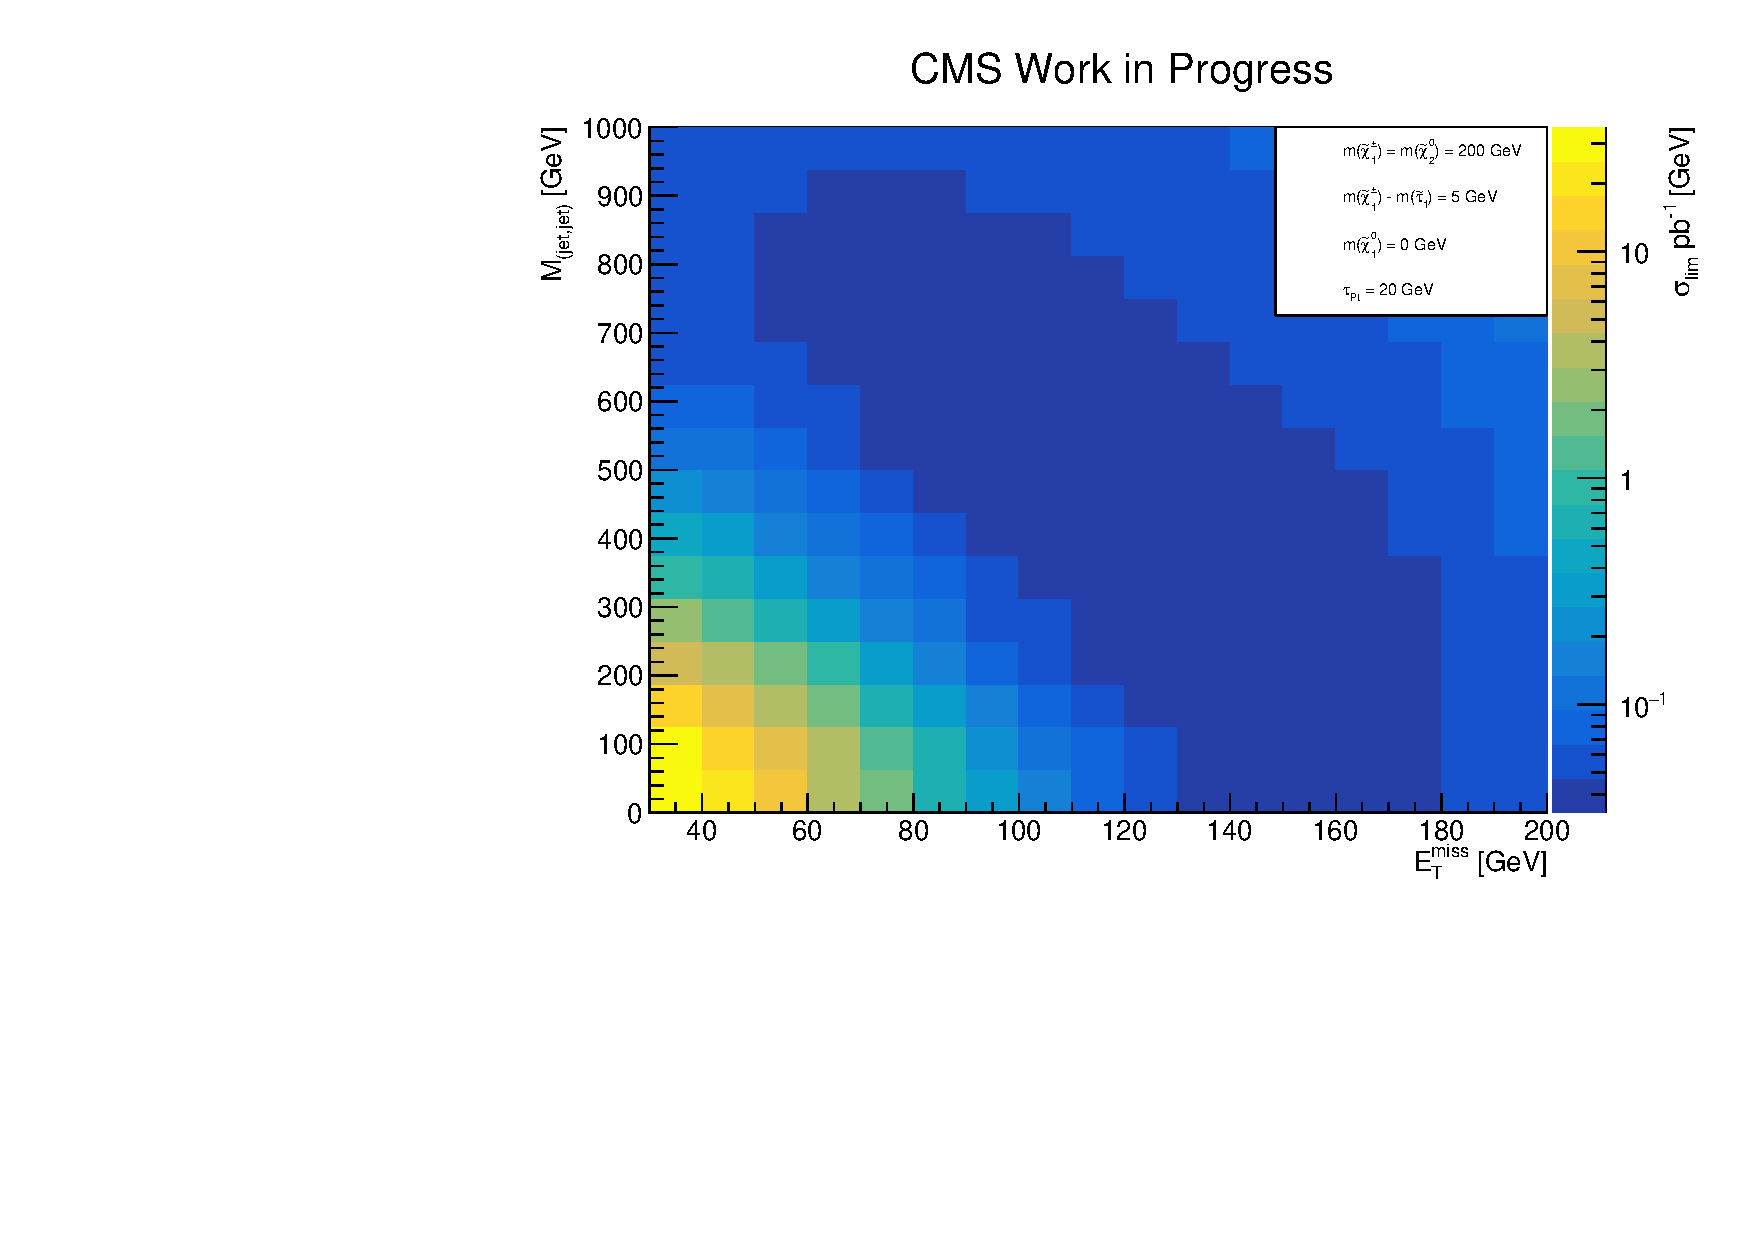
\includegraphics[width=0.45\textwidth]{analysis/pics/JetInvMass_vs_MET_xsec_chi200_lsp000_taupt20_zoom.pdf} 		
	\end{tabular}
	\caption{(Left) Cross section limit as function of $m_{jj}$ and \met for \charginopm = \neutralinotwo = 200 GeV, \neutralinoone = 0 GeV and an offline selection on $\pt(\hadtau) <  20\gev$. (Right) Zooming into the minimum cross section limit area for the same benchmark point.}
	\label{fig::JetInvMass_vs_MET_xsec_chi200_lsp000_taupt20}
\end{figure}

\begin{figure}[tbh!]
	\centering
	\begin{tabular}{cc}
		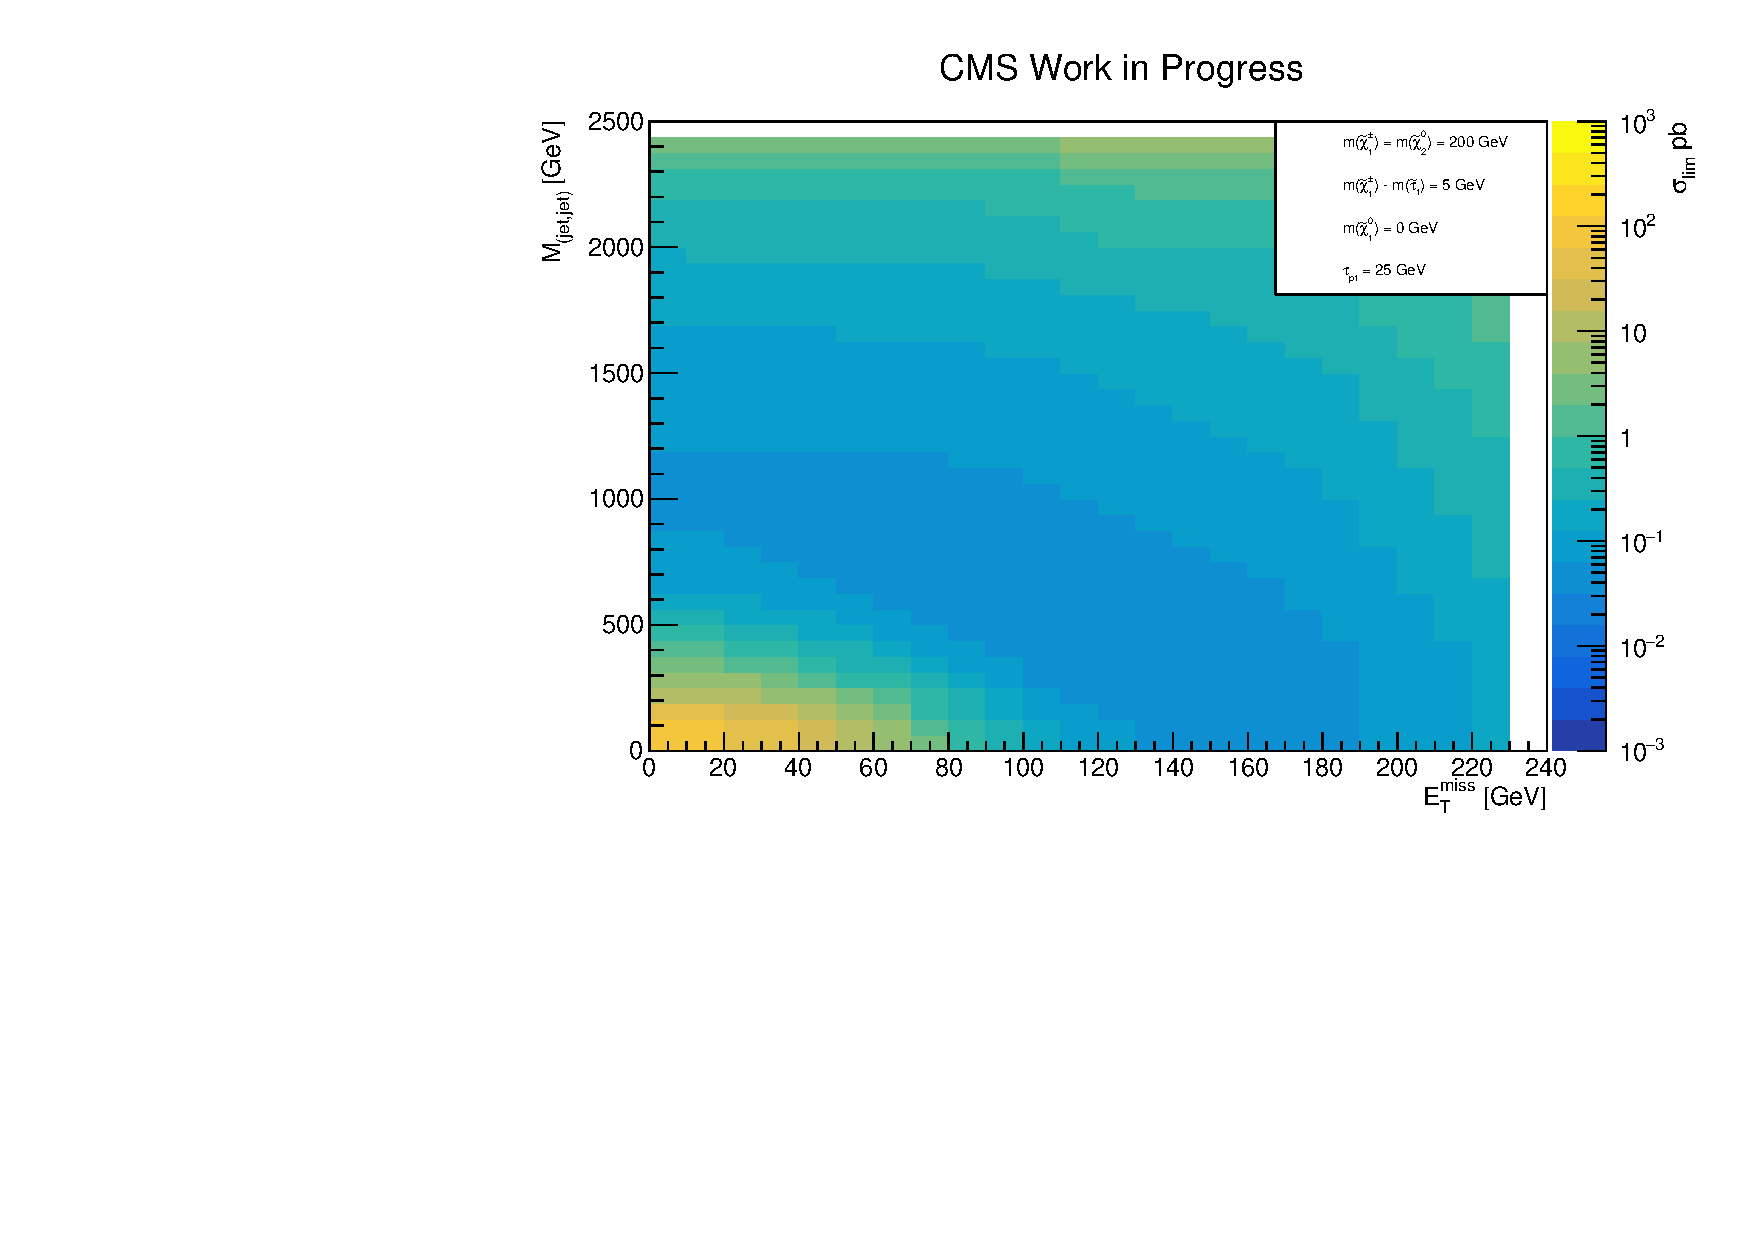
\includegraphics[width=0.45\textwidth]{analysis/pics/JetInvMass_vs_MET_xsec_chi200_lsp000_taupt25.pdf}
		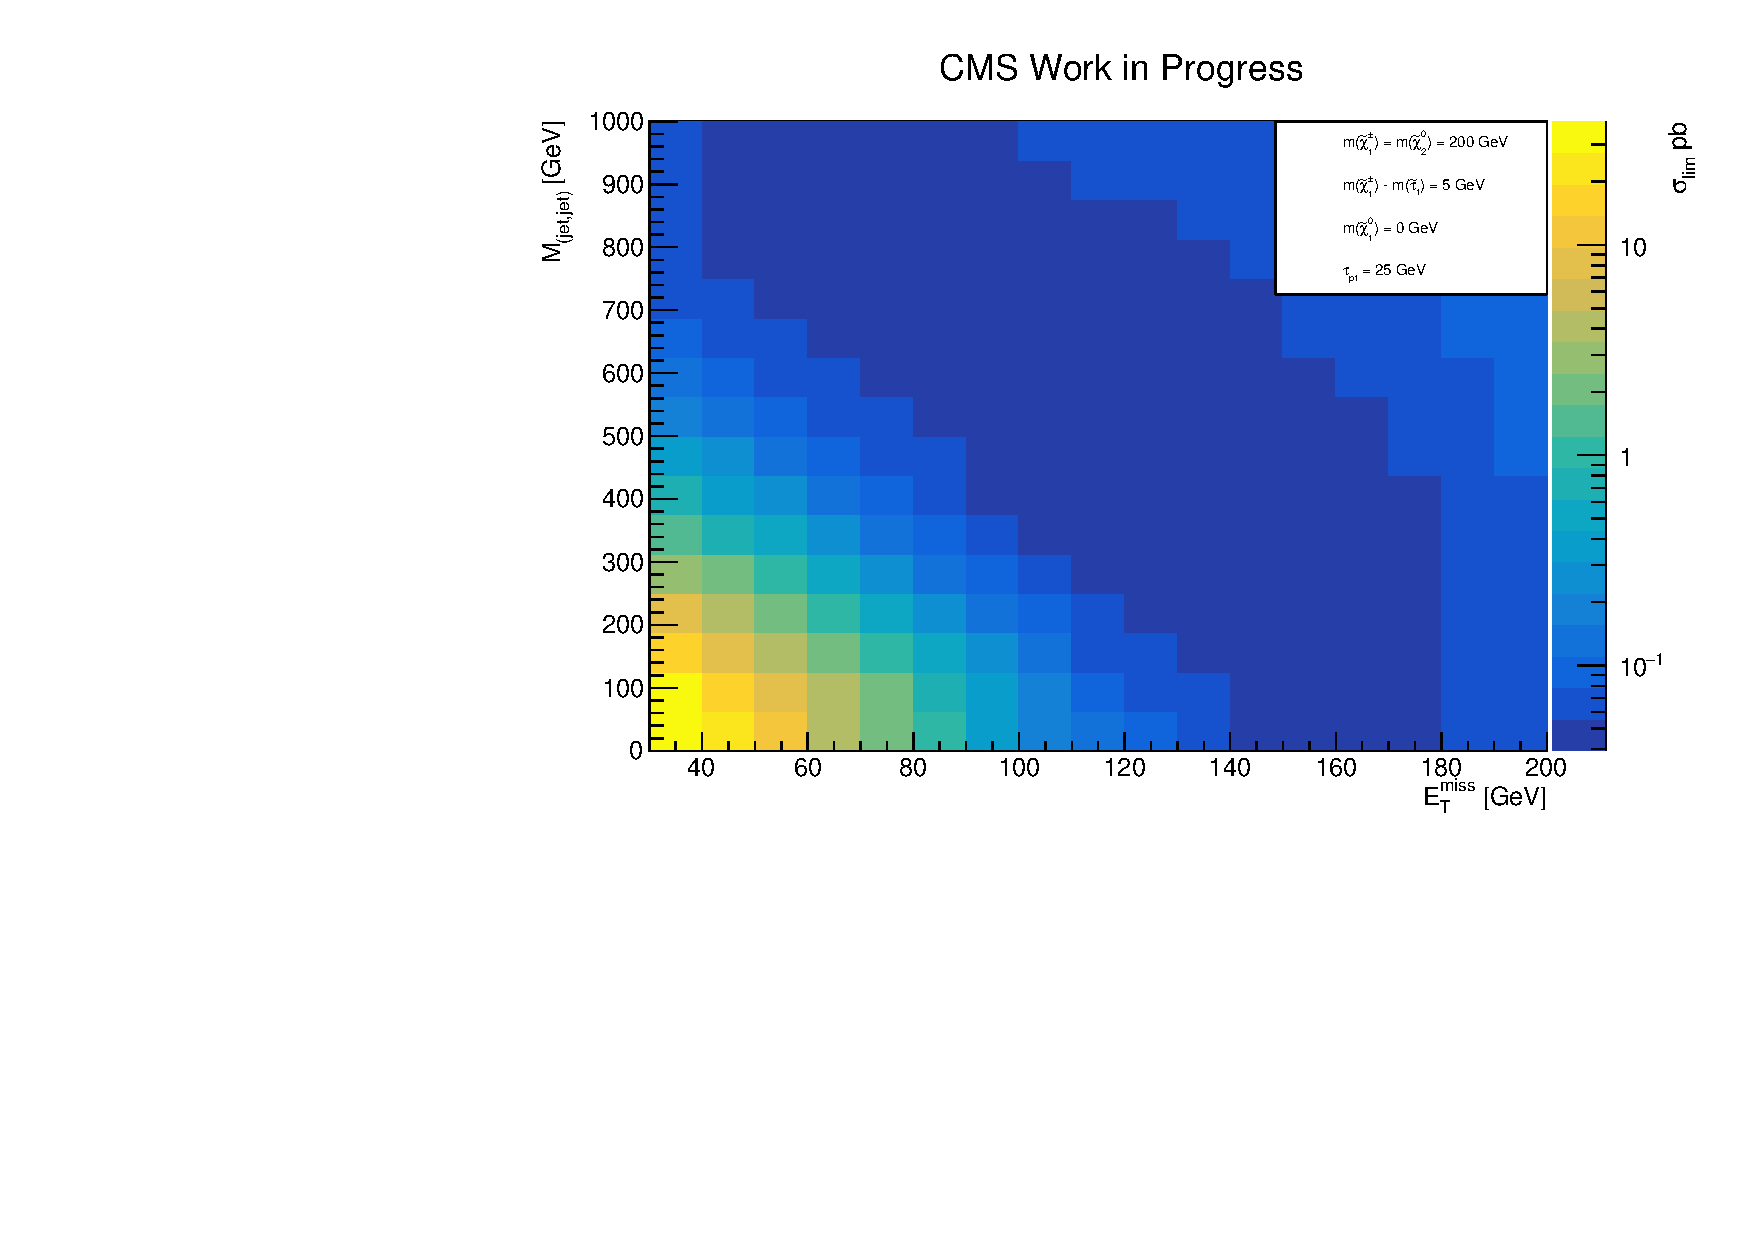
\includegraphics[width=0.45\textwidth]{analysis/pics/JetInvMass_vs_MET_xsec_chi200_lsp000_taupt25_zoom.pdf} 		
	\end{tabular}
	\caption{(Left) Cross section limit as function of $m_{jj}$ and \met for \charginopm = \neutralinotwo = 200 GeV, \neutralinoone = 0 GeV and an offline selection on $\pt(\hadtau) <  25\gev$. (Right) Zooming into the minimum cross section limit area for the same benchmark point.}
	\label{fig::JetInvMass_vs_MET_xsec_chi200_lsp000_taupt25}
\end{figure}

\begin{figure}[tbh!]
	\centering
	\begin{tabular}{cc}
		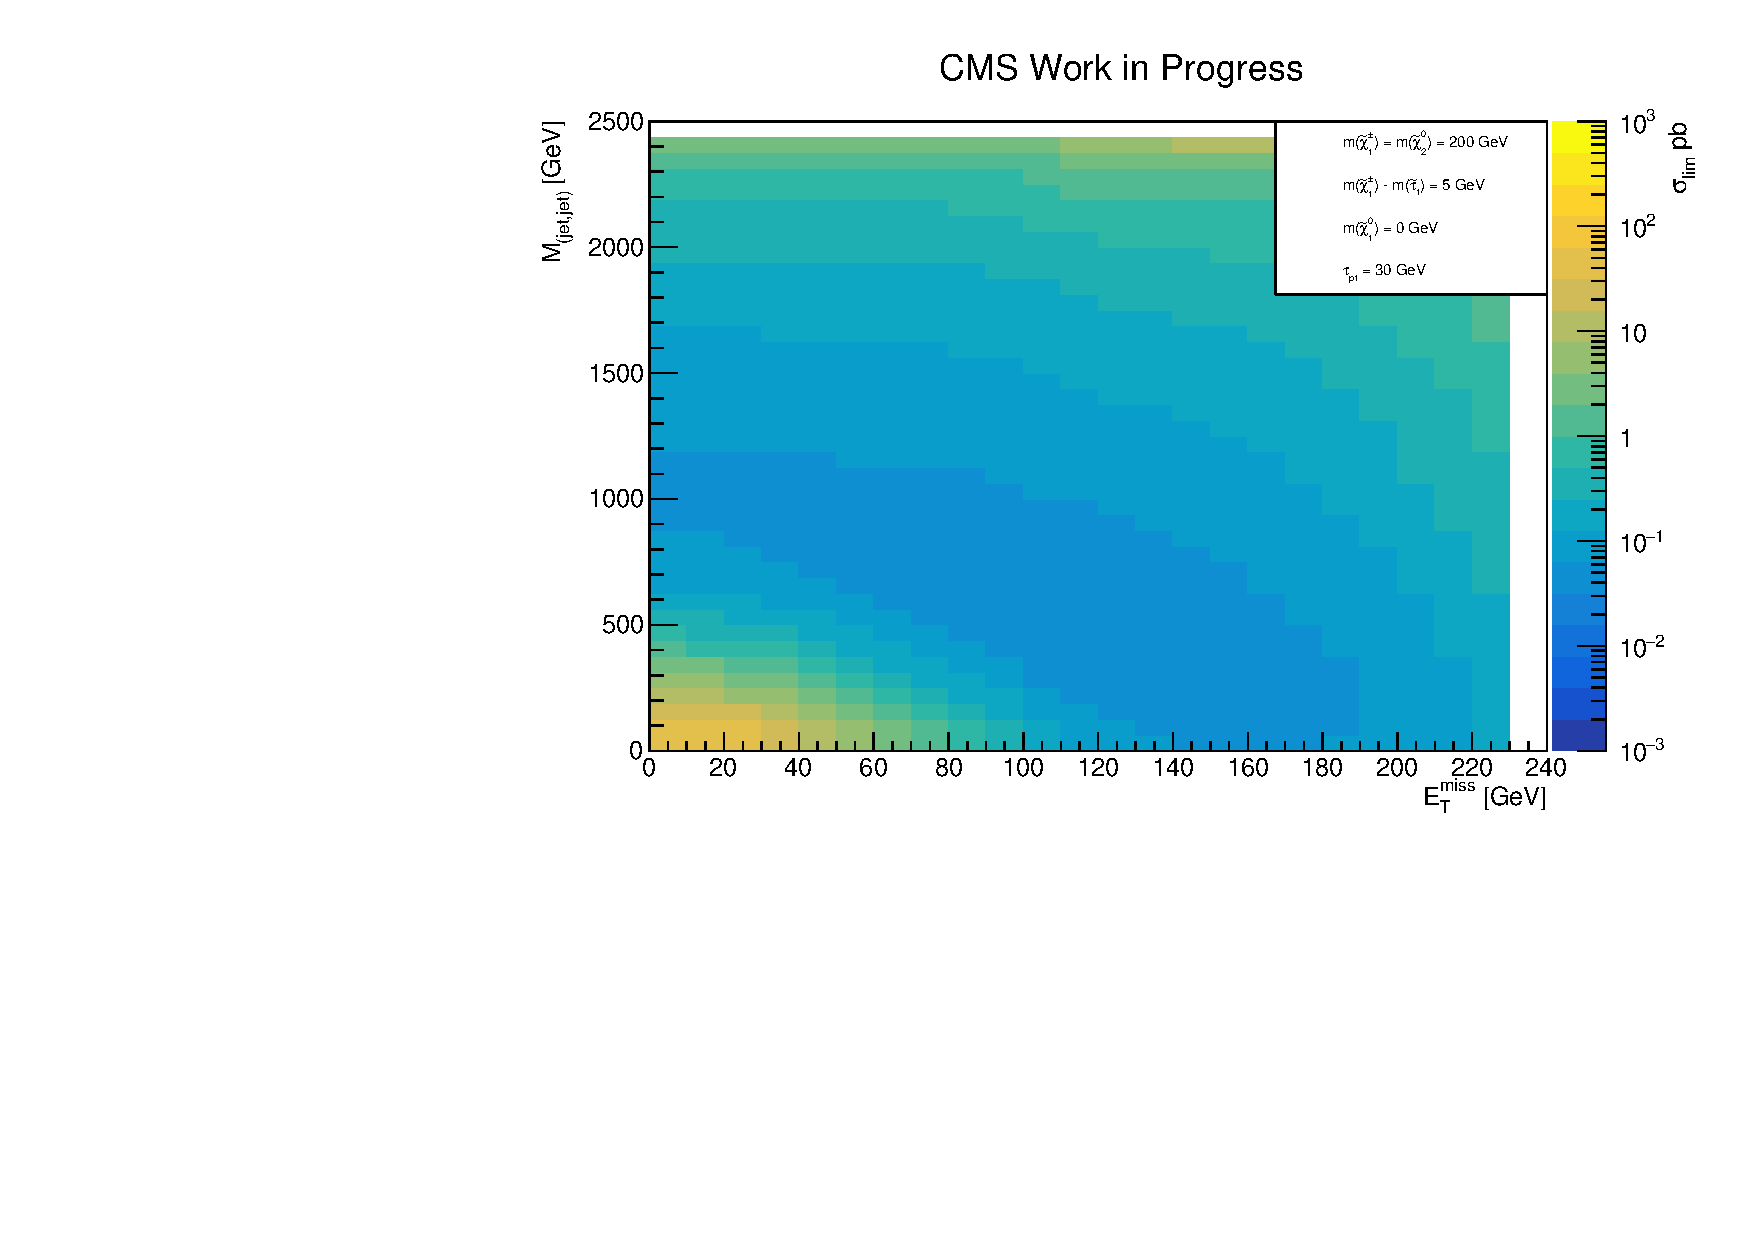
\includegraphics[width=0.45\textwidth]{analysis/pics/JetInvMass_vs_MET_xsec_chi200_lsp000_taupt30.pdf}
		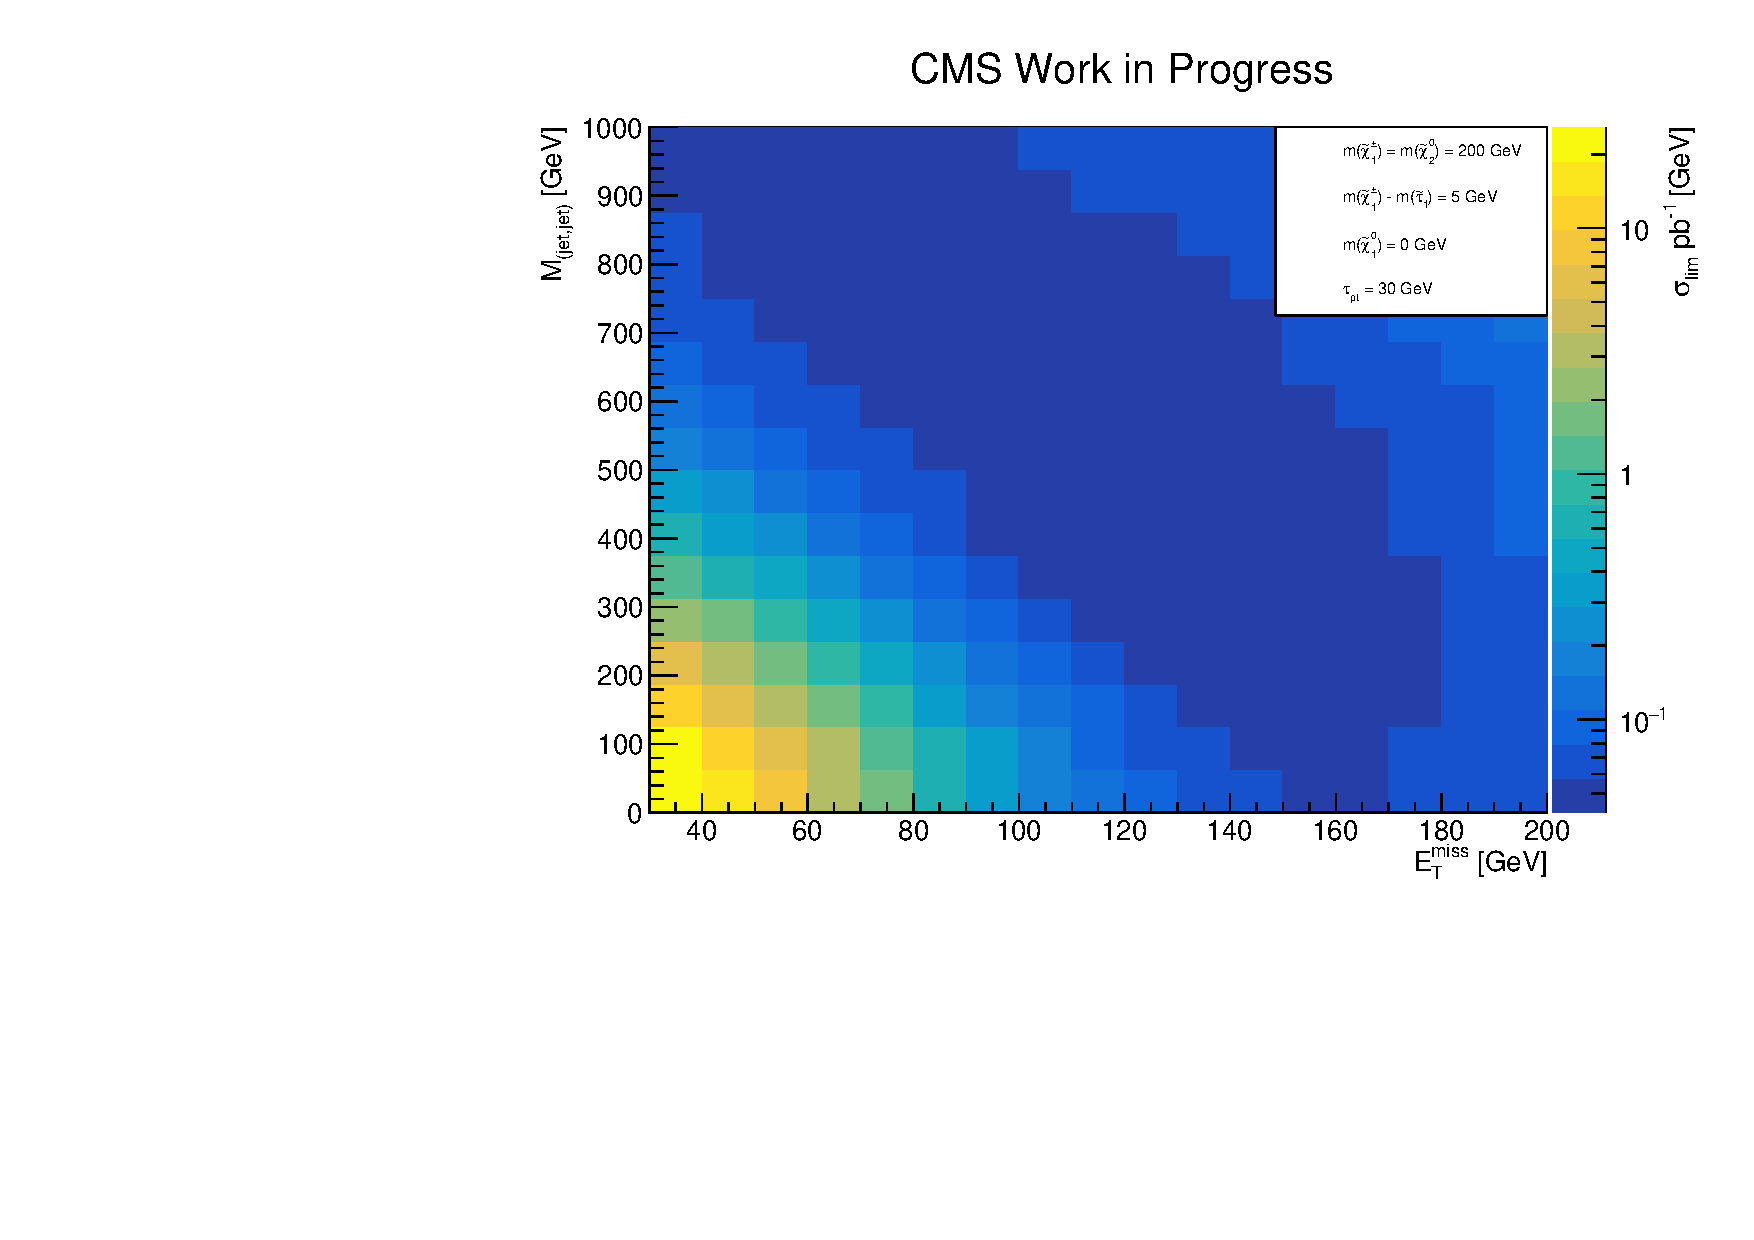
\includegraphics[width=0.45\textwidth]{analysis/pics/JetInvMass_vs_MET_xsec_chi200_lsp000_taupt30_zoom.pdf} 		
	\end{tabular}
	\caption{(Left) Cross section limit as function of $m_{jj}$ and \met for \charginopm = \neutralinotwo = 200 GeV, \neutralinoone = 0 GeV and an offline selection on $\pt(\hadtau) <  30\gev$. (Right) Zooming into the minimum cross section limit area for the same benchmark point.}
	\label{fig::JetInvMass_vs_MET_xsec_chi200_lsp000_taupt30}
\end{figure}

\begin{figure}[tbh!]
	\centering
	\begin{tabular}{cc}
		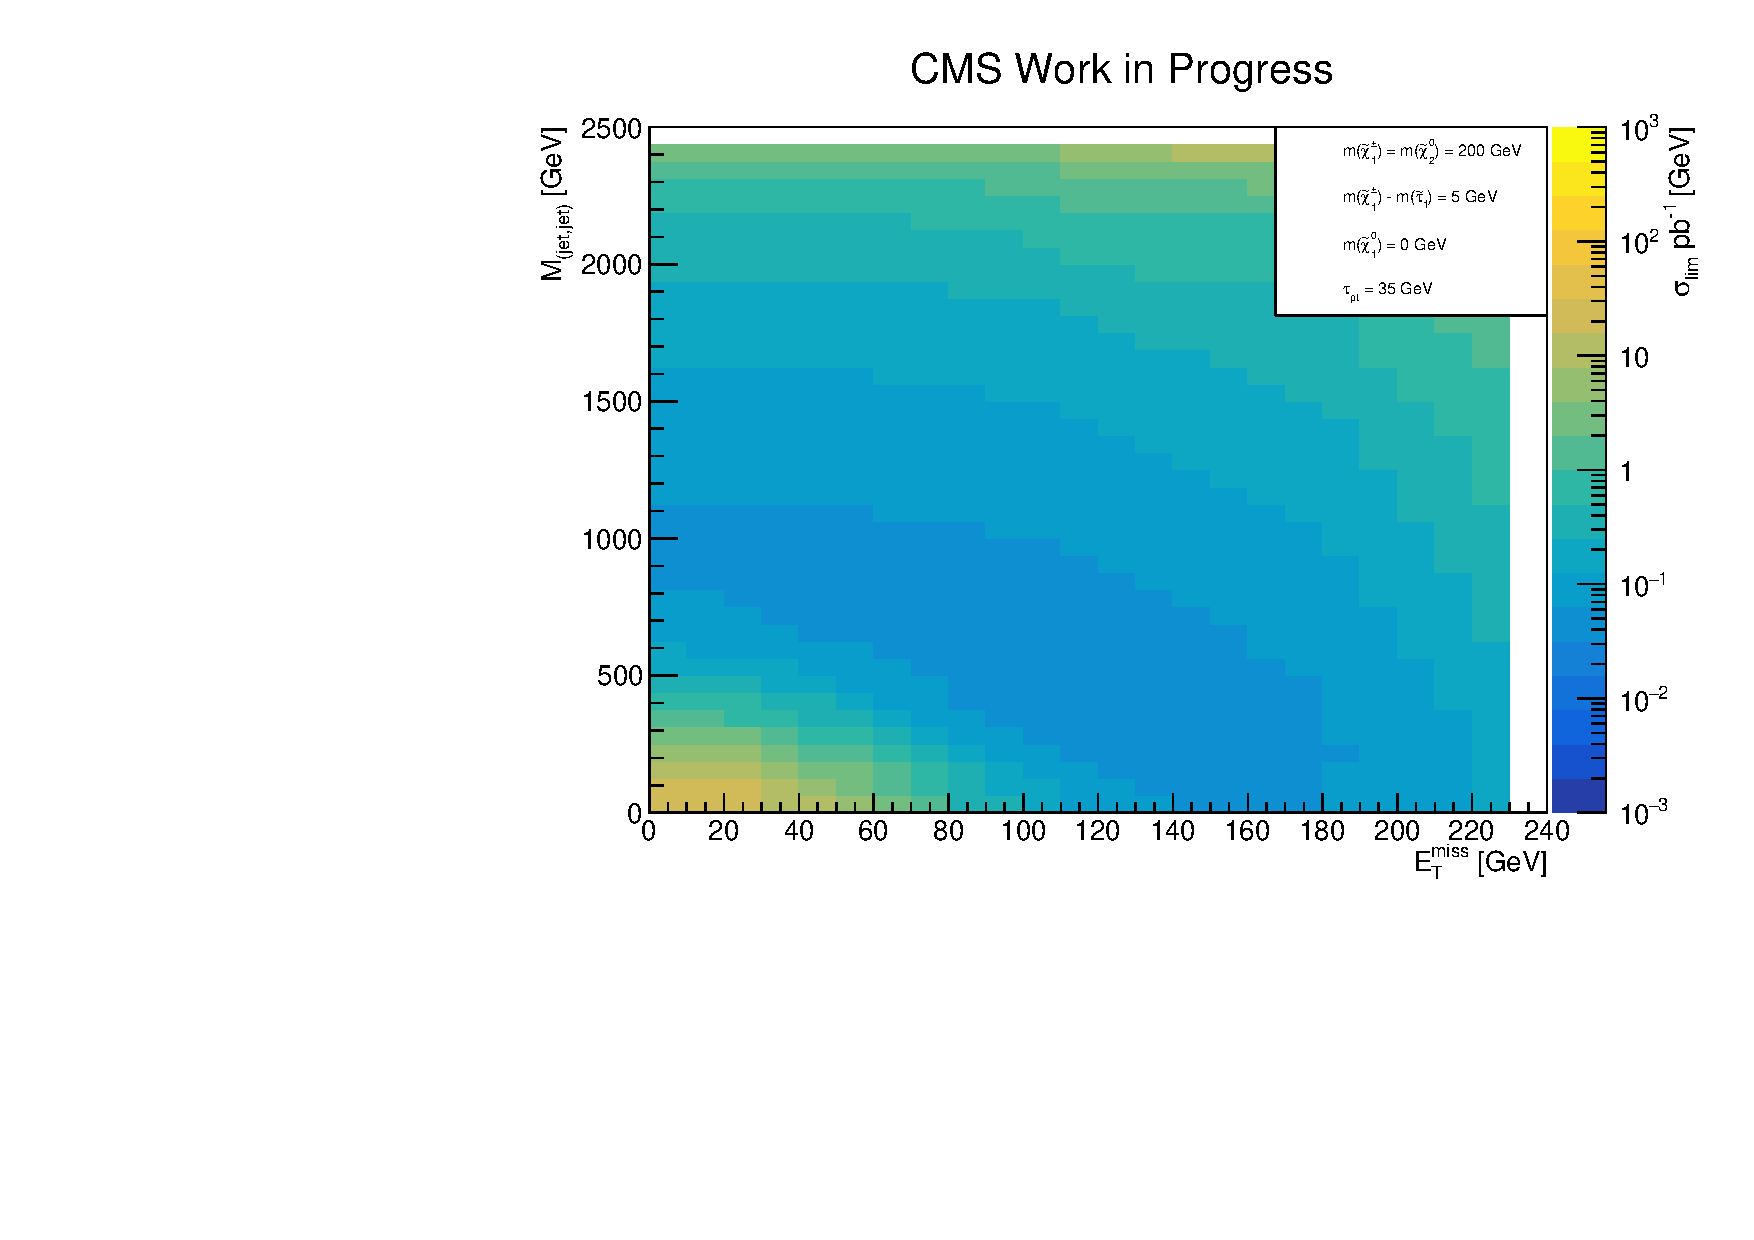
\includegraphics[width=0.45\textwidth]{analysis/pics/JetInvMass_vs_MET_xsec_chi200_lsp000_taupt35.pdf}
		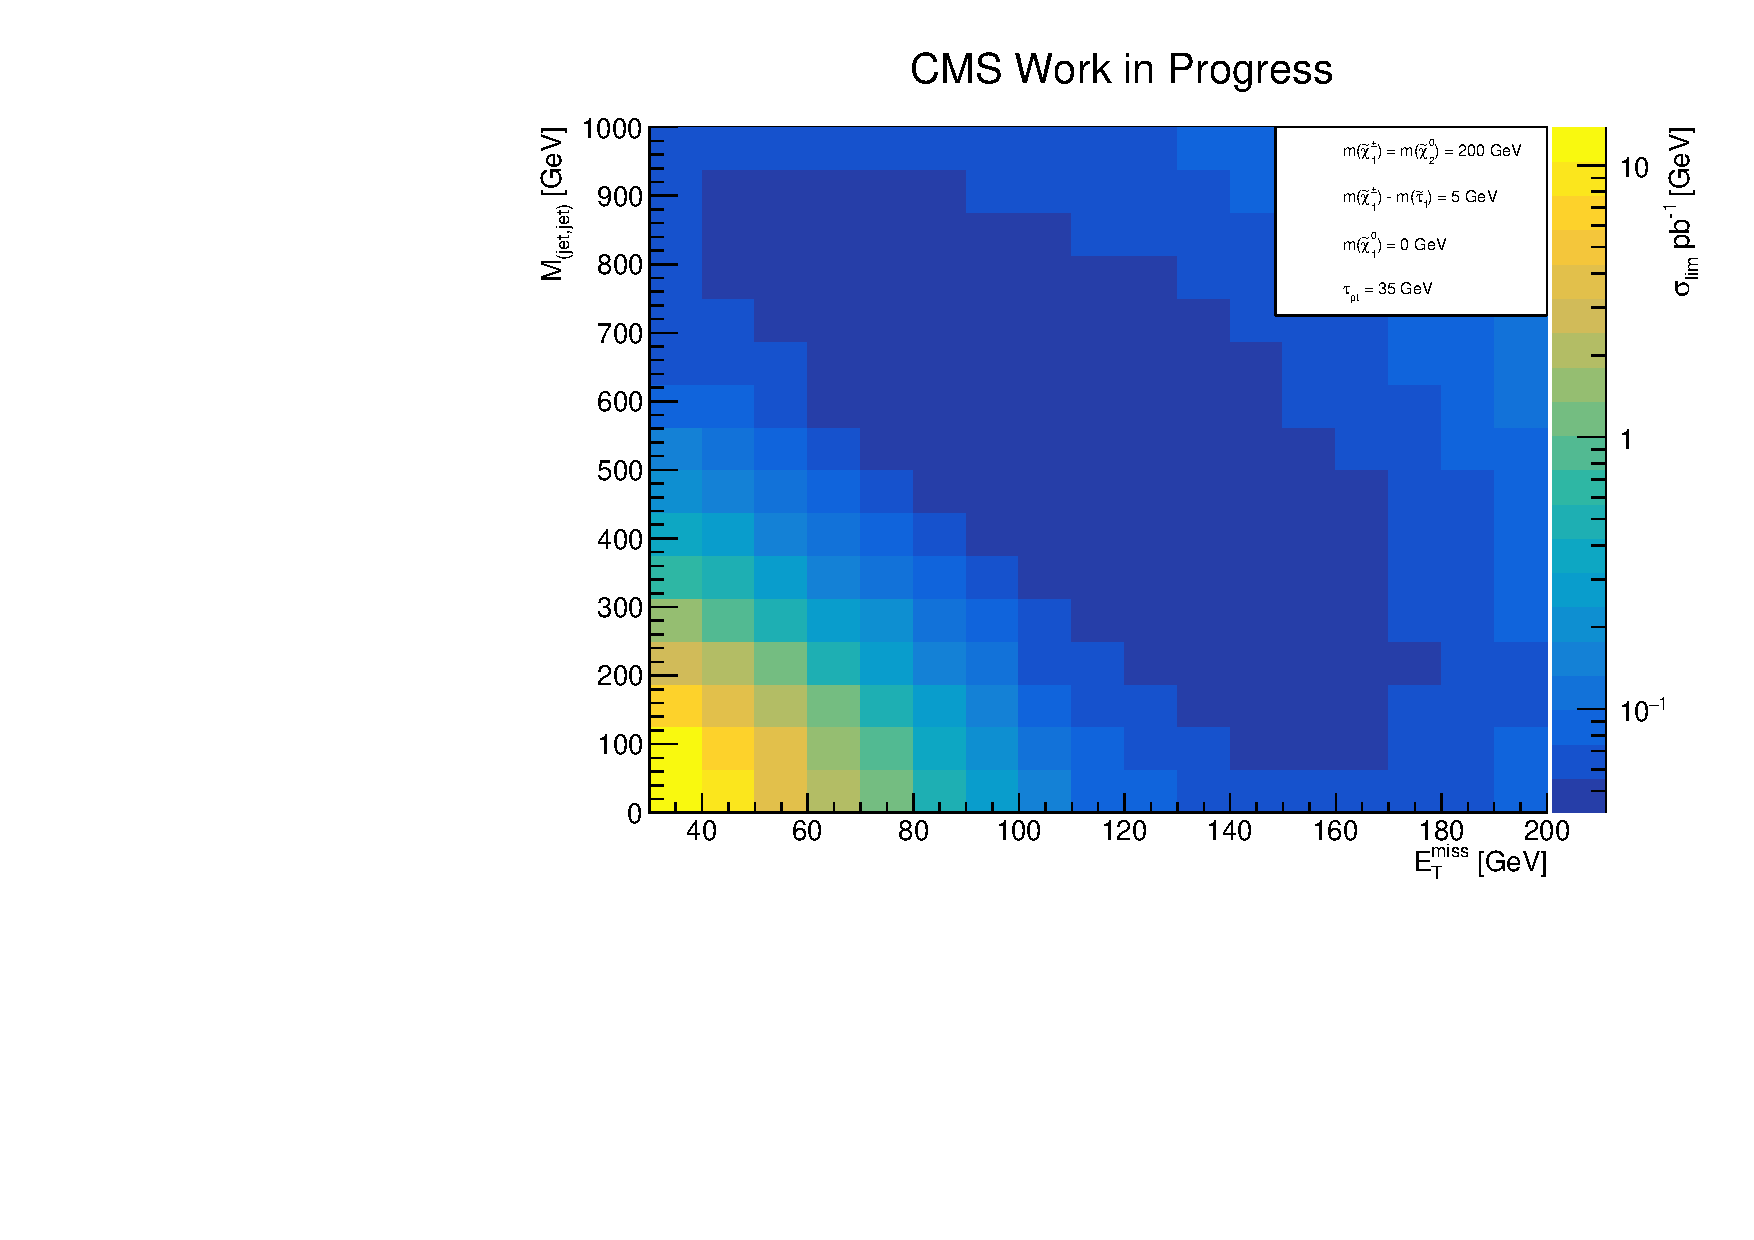
\includegraphics[width=0.45\textwidth]{analysis/pics/JetInvMass_vs_MET_xsec_chi200_lsp000_taupt35_zoom.pdf} 		
	\end{tabular}
	\caption{(Left) Cross section limit as function of $m_{jj}$ and \met for \charginopm = \neutralinotwo = 200 GeV, \neutralinoone = 0 GeV and an offline selection on $\pt(\hadtau) <  35\gev$. (Right) Zooming into the minimum cross section limit area for the same benchmark point.}
	\label{fig::JetInvMass_vs_MET_xsec_chi200_lsp000_taupt35}
\end{figure}

\begin{figure}[tbh!]
	\centering
	\begin{tabular}{cc}
		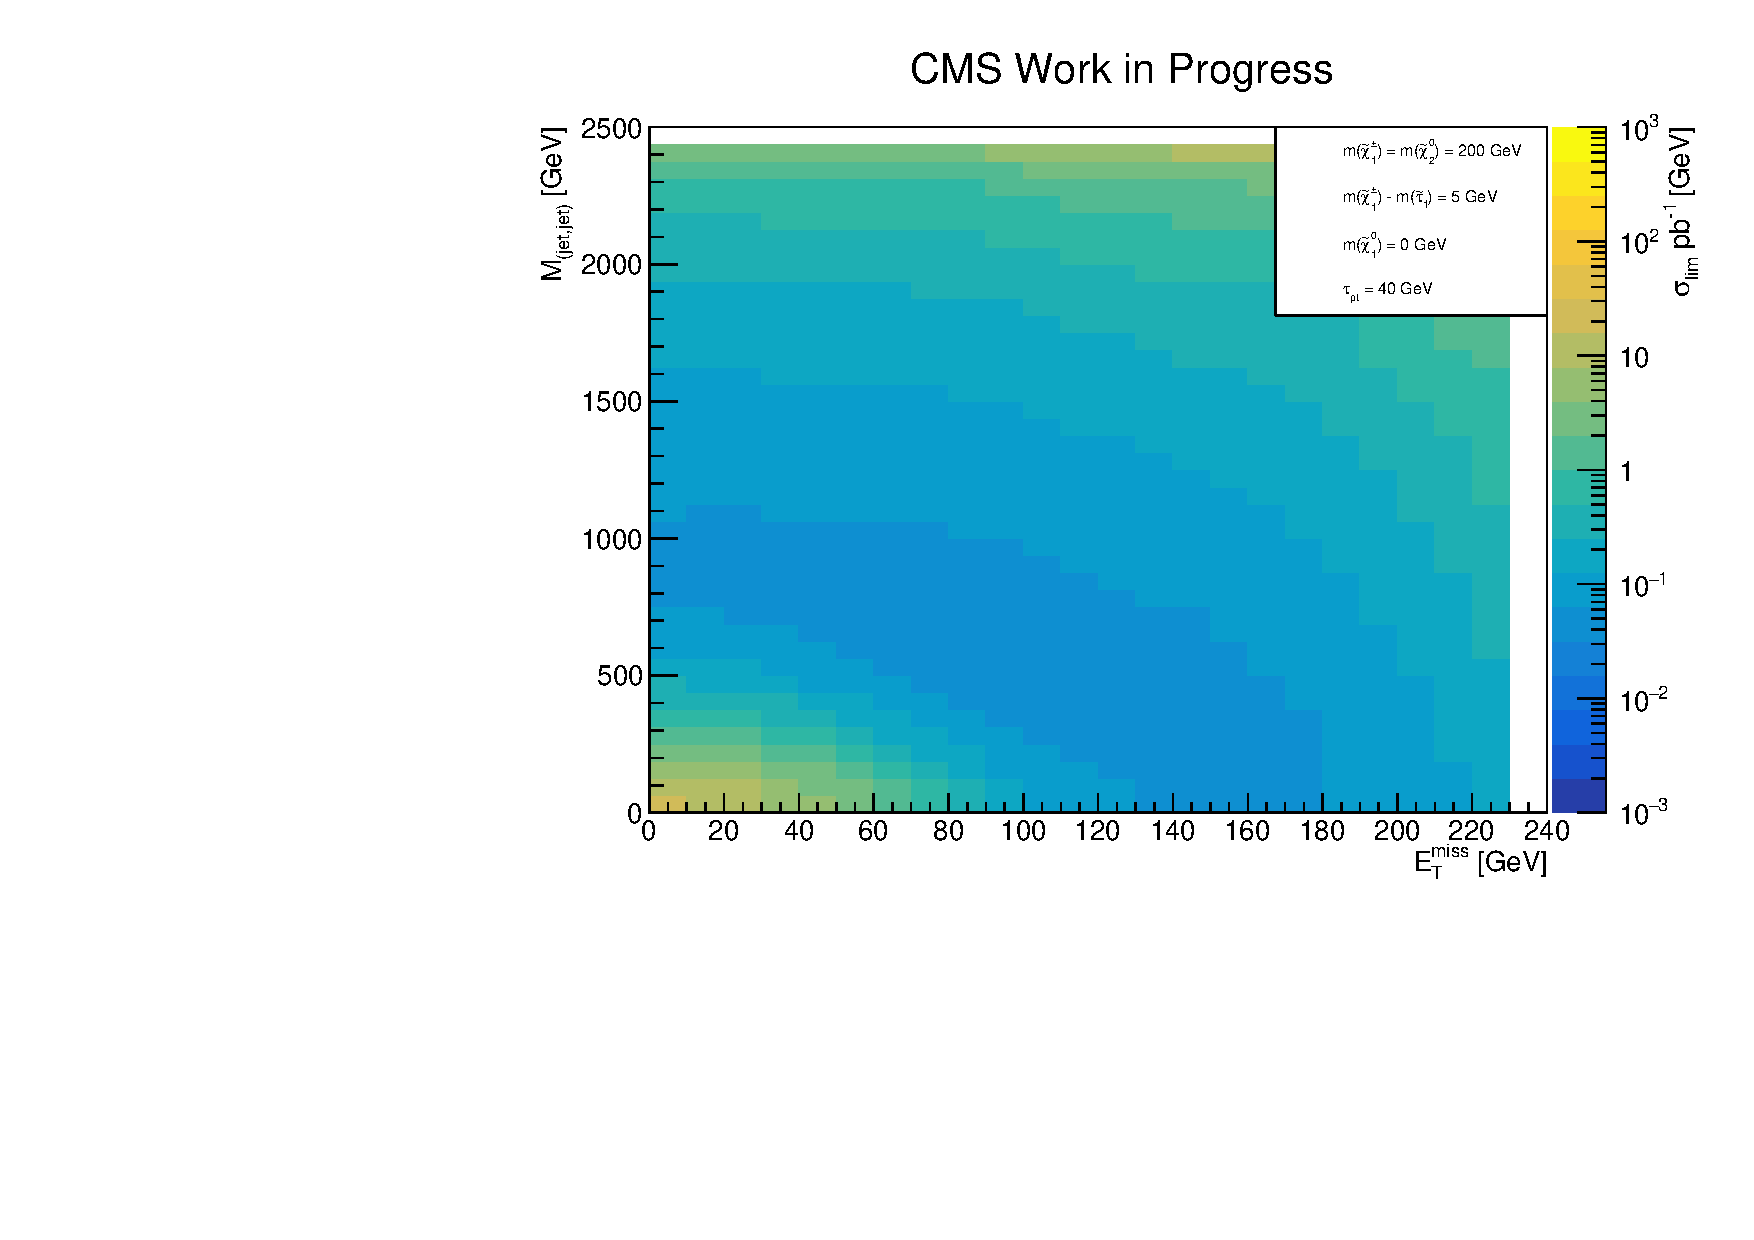
\includegraphics[width=0.45\textwidth]{analysis/pics/JetInvMass_vs_MET_xsec_chi200_lsp000_taupt40.pdf}
		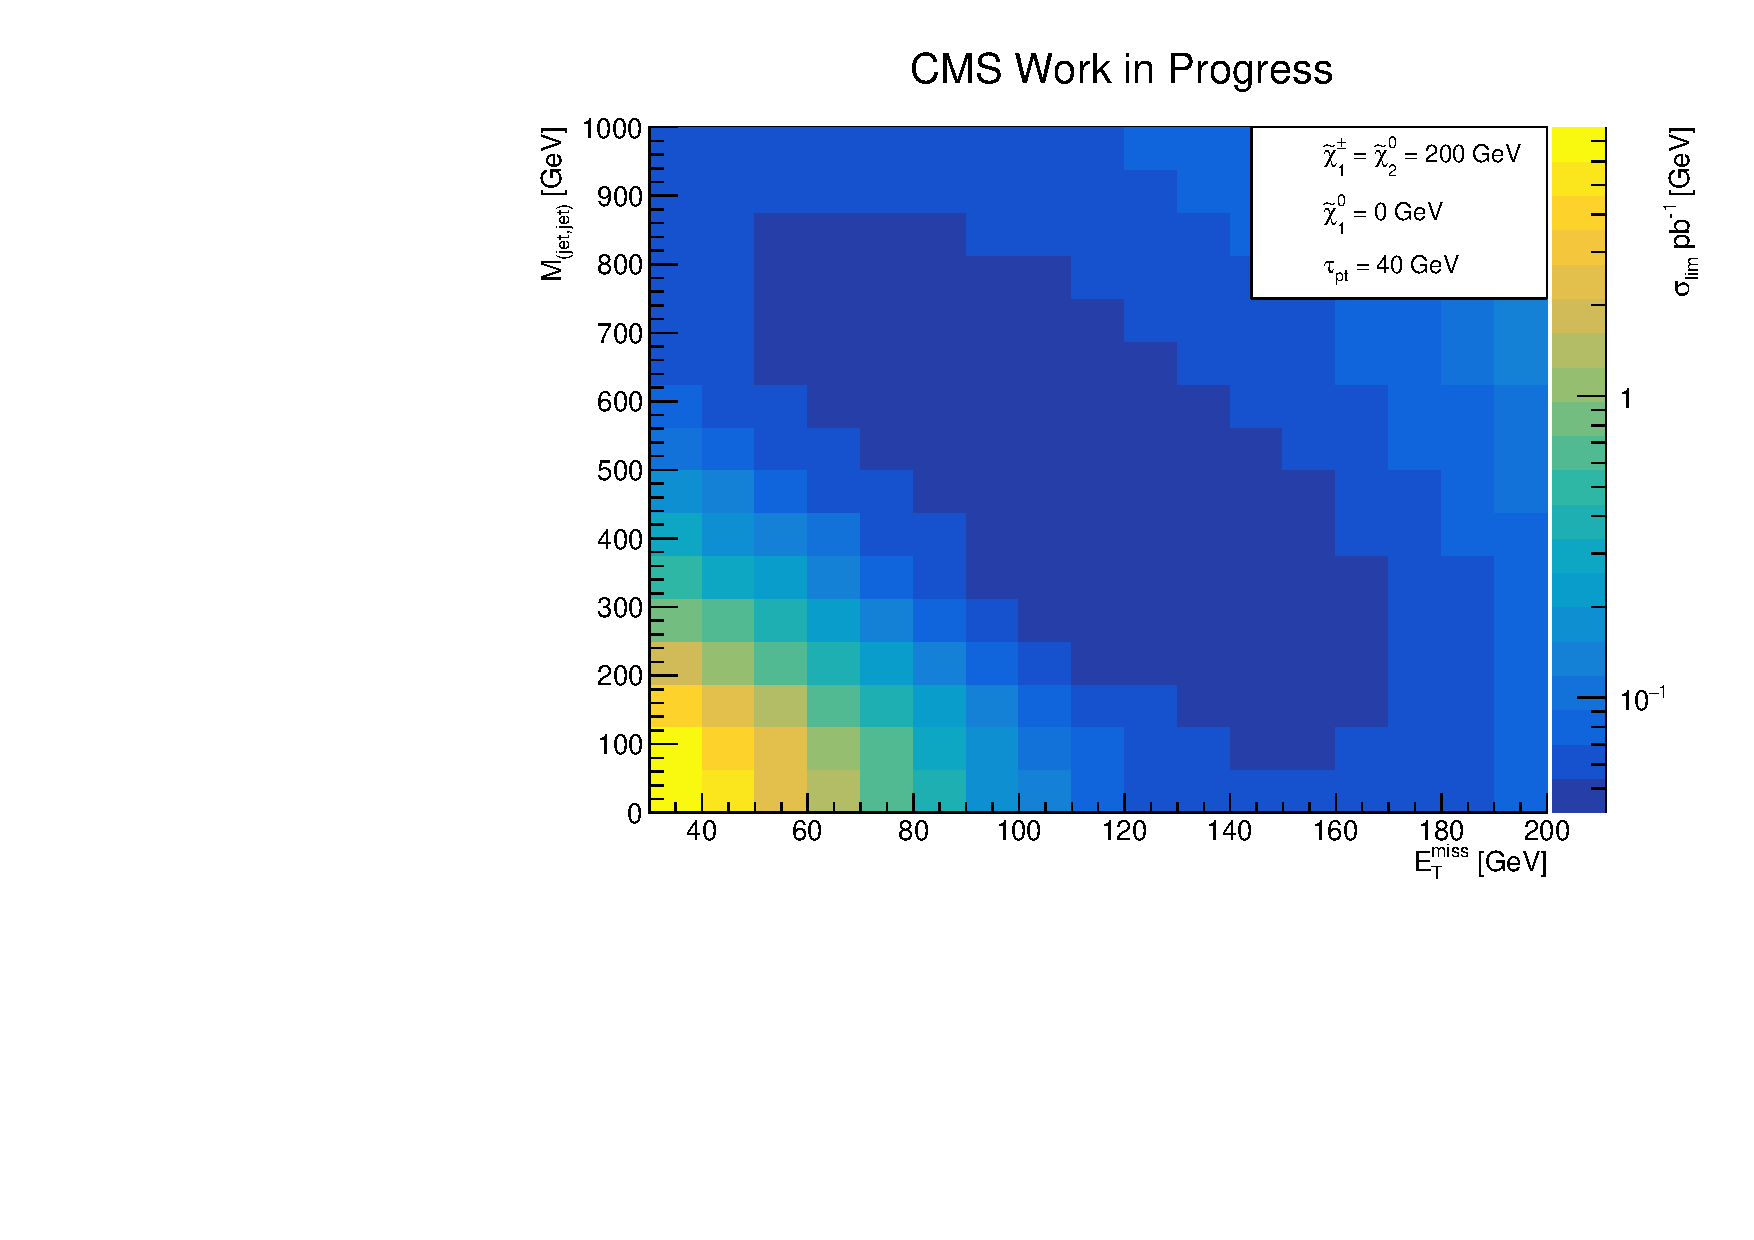
\includegraphics[width=0.45\textwidth]{analysis/pics/JetInvMass_vs_MET_xsec_chi200_lsp000_taupt40_zoom.pdf} 		
	\end{tabular}
	\caption{(Left) Cross section limit as function of $m_{jj}$ and \met for \charginopm = \neutralinotwo = 200 GeV, \neutralinoone = 0 GeV and an offline selection on $\pt(\hadtau) <  40\gev$. (Right) Zooming into the minimum cross section limit area for the same benchmark point.}
	\label{fig::JetInvMass_vs_MET_xsec_chi200_lsp000_taupt40}
\end{figure}

\begin{figure}[tbh!]
	\centering
	\begin{tabular}{cc}
		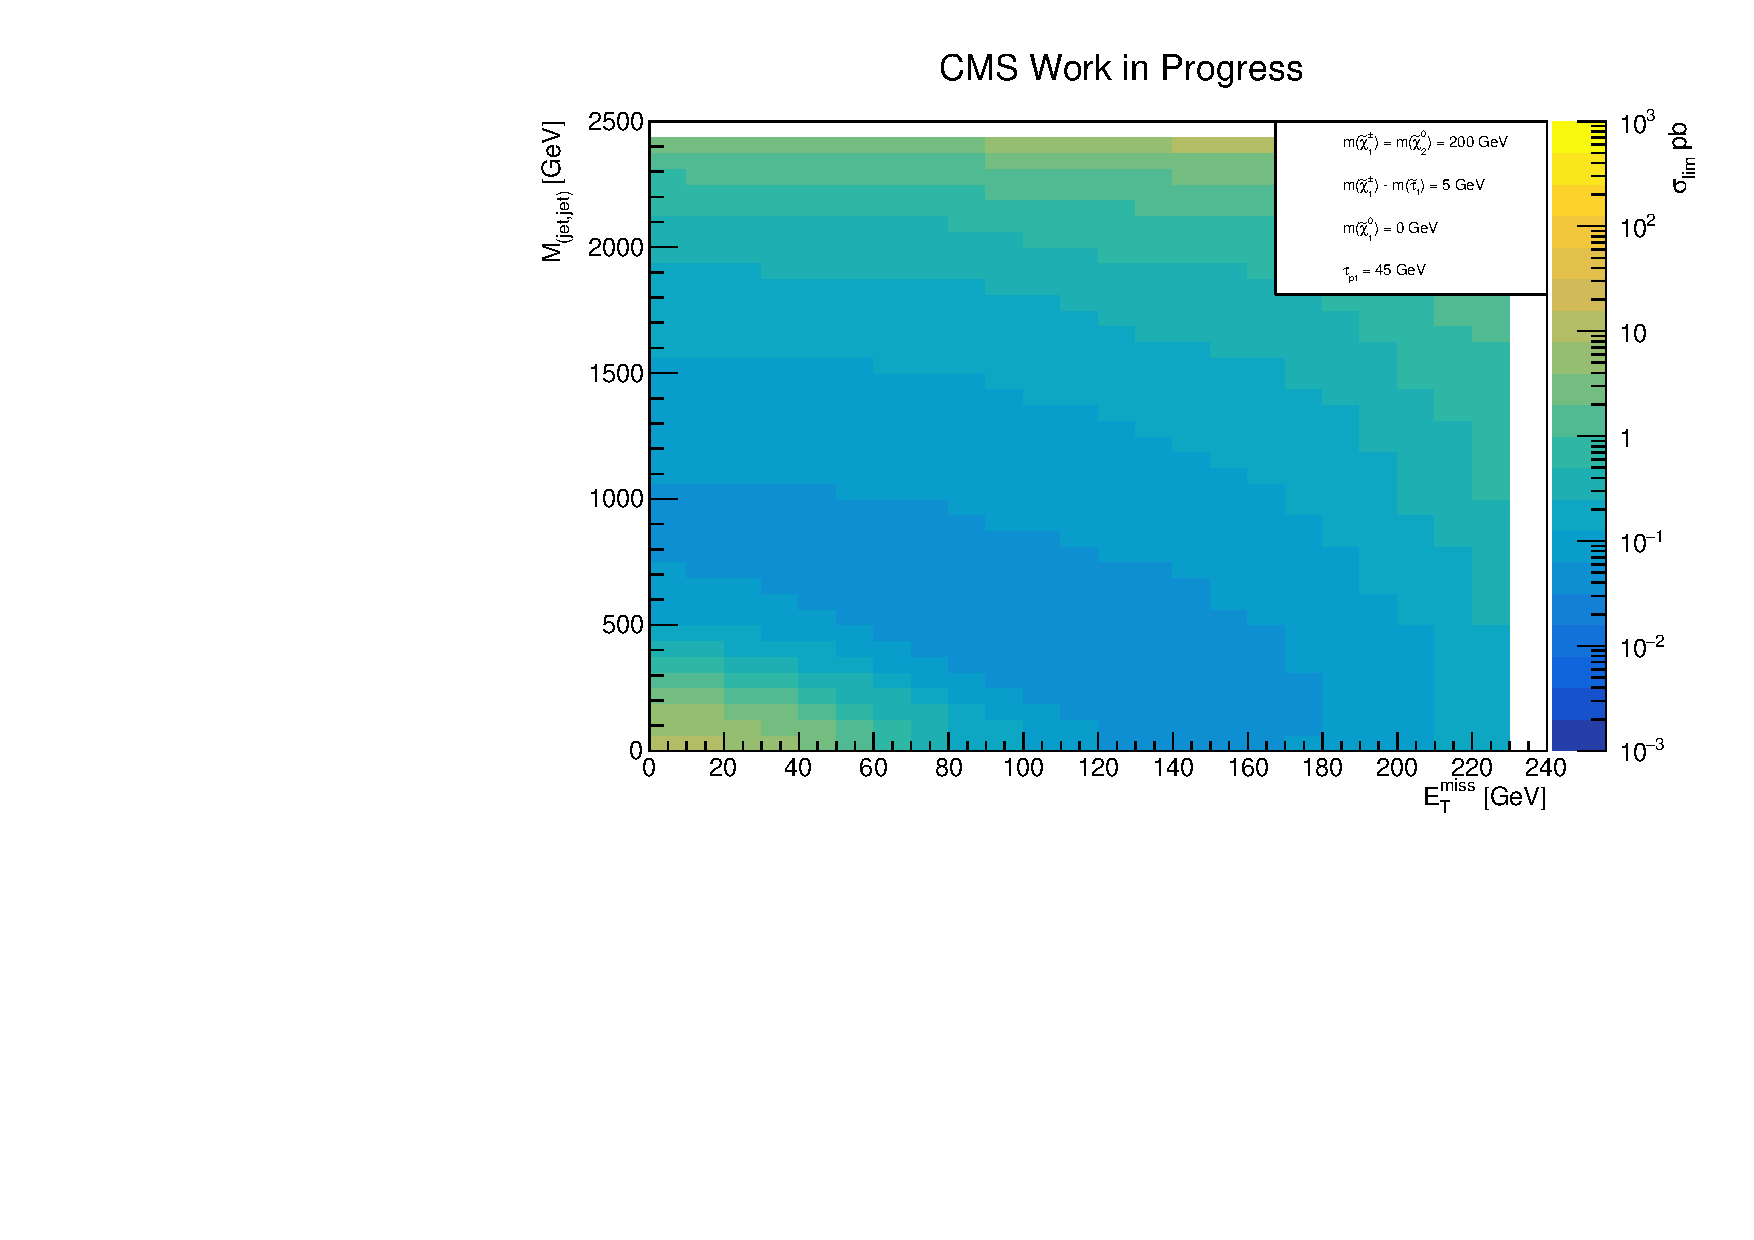
\includegraphics[width=0.45\textwidth]{analysis/pics/JetInvMass_vs_MET_xsec_chi200_lsp000_taupt45.pdf}
		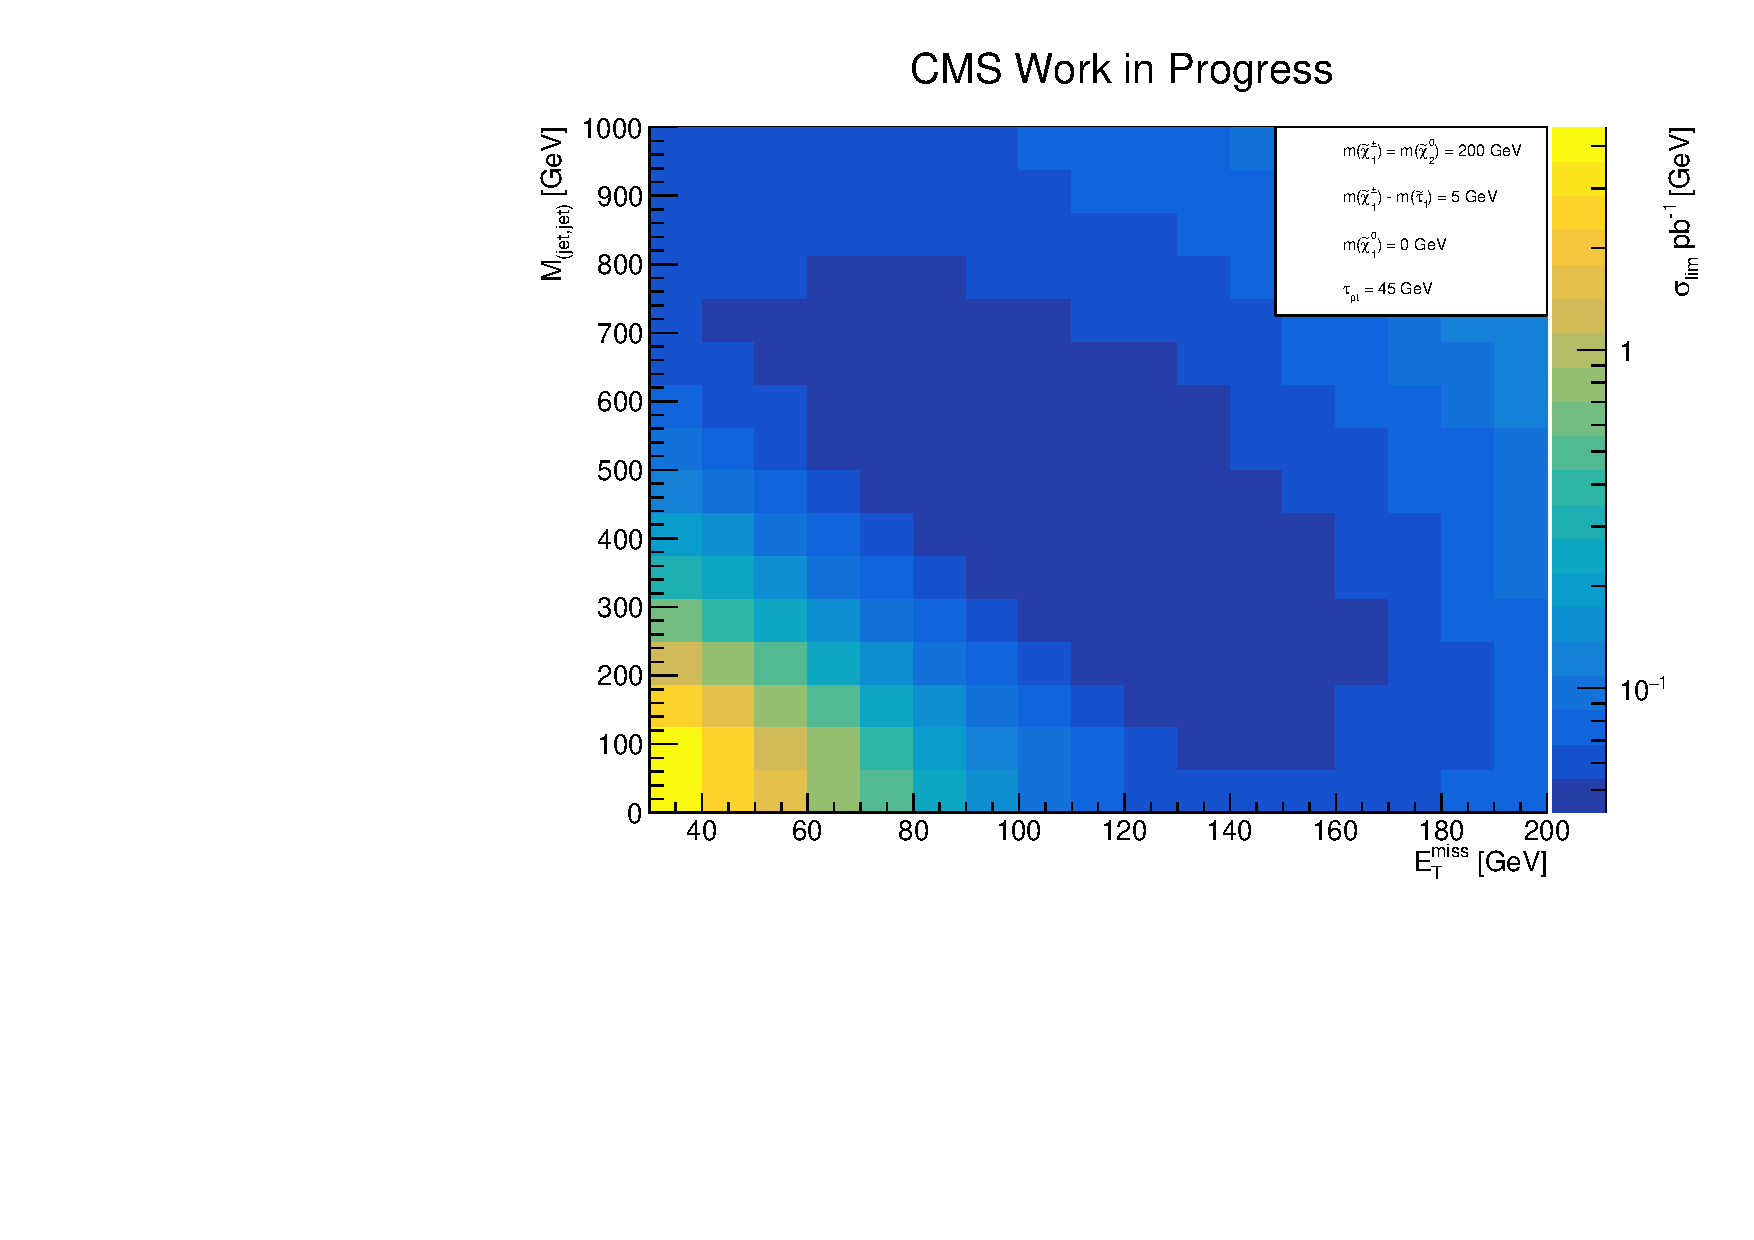
\includegraphics[width=0.45\textwidth]{analysis/pics/JetInvMass_vs_MET_xsec_chi200_lsp000_taupt45_zoom.pdf} 		
	\end{tabular}
	\caption{(Left) Cross section limit as function of $m_{jj}$ and \met for \charginopm = \neutralinotwo = 200 GeV, \neutralinoone = 0 GeV and an offline selection on $\pt(\hadtau) <  45\gev$. (Right) Zooming into the minimum cross section limit area for the same benchmark point.}
	\label{fig::JetInvMass_vs_MET_xsec_chi200_lsp000_taupt45}
\end{figure}

\FloatBarrier

\subsection*{\charginopm = \neutralinotwo = 300 GeV, \neutralinoone = 0 GeV}

\FloatBarrier

\begin{table}
	\begin{center}
		
		
		\begin{tabular}{| c | c | c | c | }
			\toprule
			\multicolumn{4}{| c | }{m(\charginopm) = m(\neutralinotwo) = 300\gev; m(\neutralinoone) = 0\gev} \\
			\midrule
			$\sigma_{lim}^{min}\pm(stat.)\pm(MC syst.)$ [pb]  & \pt(\hadtau) [GeV] & \mjj [GeV] & \met [GeV] \\
			\midrule
			$0.0345751\pm0.00701739^{+0.0032299}_{-0.00382075}$ & $<$ 20 & $<$ 312.5  & $<$ 120 \\
			
			$0.041228\pm0.00895289^{+0.00404347}_{-0.0047528}$ & $<$ 25 & $<$ 312.5  & $<$ 130 \\
			
			$0.0429305\pm0.0069006^{+0.00326412}_{-0.0039582}$ & $<$ 30 & $<$ 437.5  & $<$ 120 \\
			
			$0.0433003\pm0.00549324^{+0.00274178}_{-0.003387}$ & $<$ 35 & $<$ 437.5  & $<$ 120 \\
			
			$0.0441397\pm0.00856017^{+0.00398096}_{-0.00473039}$ & $<$ 40 & $<$ 312.5  & $<$ 120 \\
			
			$0.0451021\pm0.00746158^{+0.00356799}_{-0.00430736}$ & $<$ 45 & $<$ 312.5  & $<$ 120 \\
			
			\bottomrule
		\end{tabular}\caption{Cross section limit minimum reached at the given cuts for $m_{jj}$, \met and an increasing \pt(\hadtau) for \charginopm = \neutralinotwo = 300 GeV, \neutralinoone = 0 GeV benchmark point.}
		\label{table::xseclimmin_chi300_lsp000}
	\end{center}
\end{table}

\begin{figure}[tbh!]
	\centering
	\begin{tabular}{cc}
		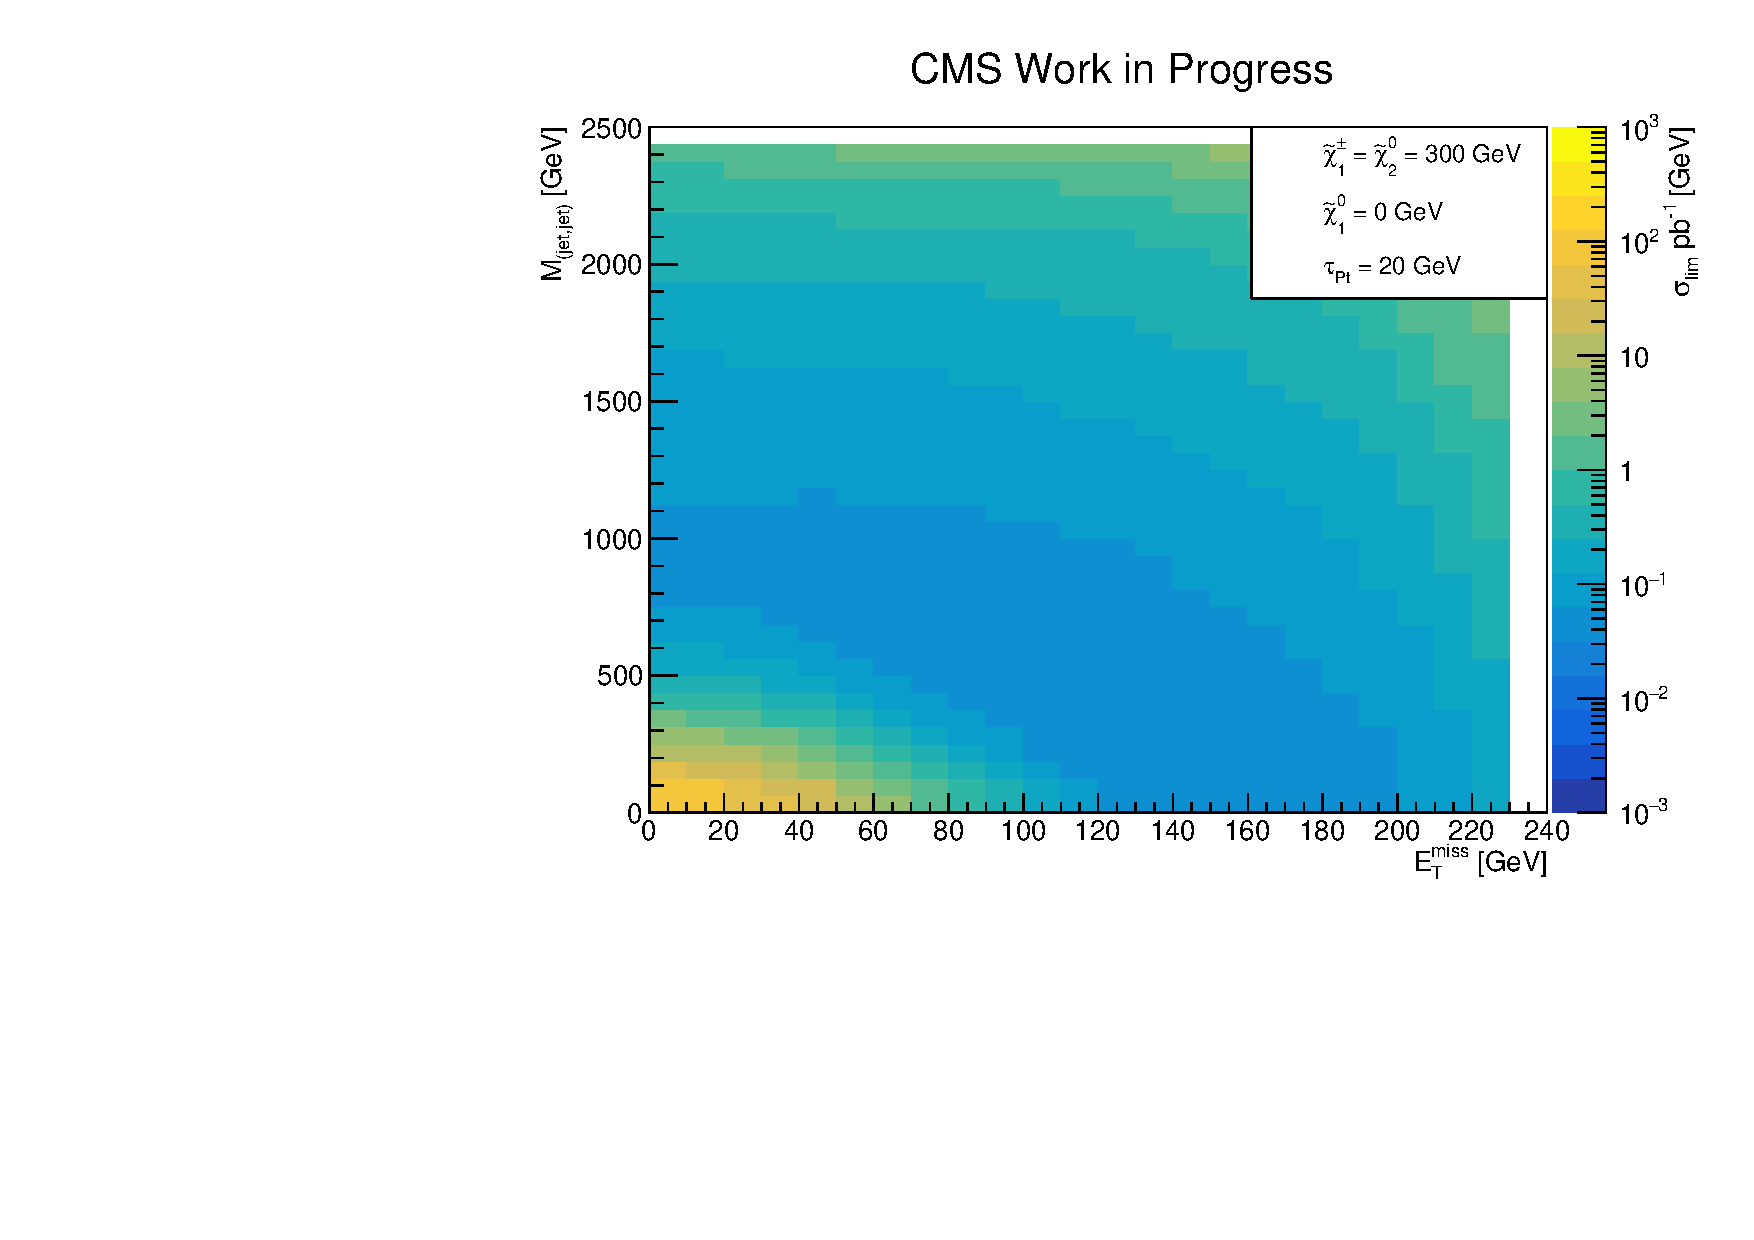
\includegraphics[width=0.45\textwidth]{analysis/pics/JetInvMass_vs_MET_xsec_chi300_lsp000_taupt20.pdf}
		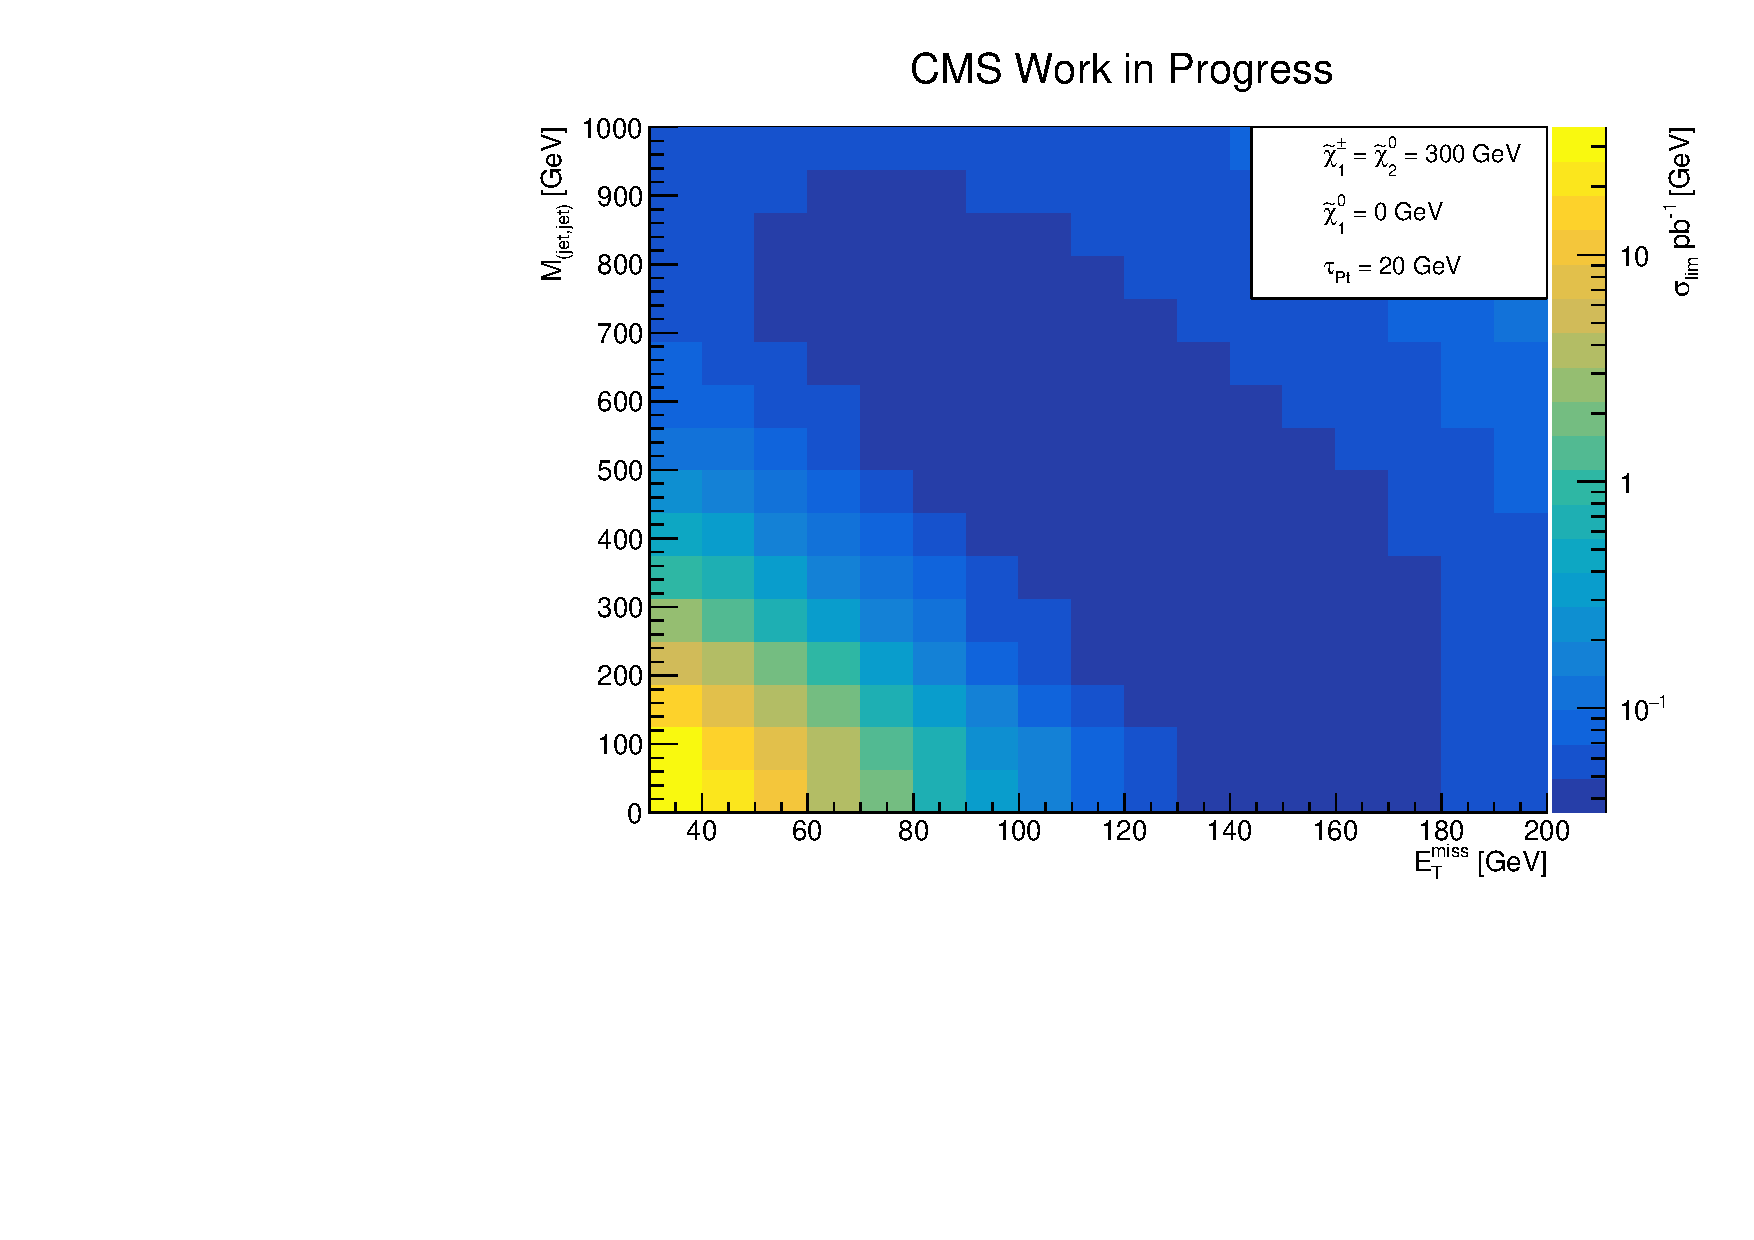
\includegraphics[width=0.45\textwidth]{analysis/pics/JetInvMass_vs_MET_xsec_chi300_lsp000_taupt20_zoom.pdf} 		
	\end{tabular}
	\caption{(Left) Cross section limit as function of $m_{jj}$ and \met for \charginopm = \neutralinotwo = 300 GeV, \neutralinoone = 0 GeV and an offline selection on $\pt(\hadtau) <  20\gev$. (Right) Zooming into the minimum cross section limit area for the same benchmark point.}
	\label{fig::JetInvMass_vs_MET_xsec_chi300_lsp000_taupt20}
\end{figure}

\begin{figure}[tbh!]
	\centering
	\begin{tabular}{cc}
		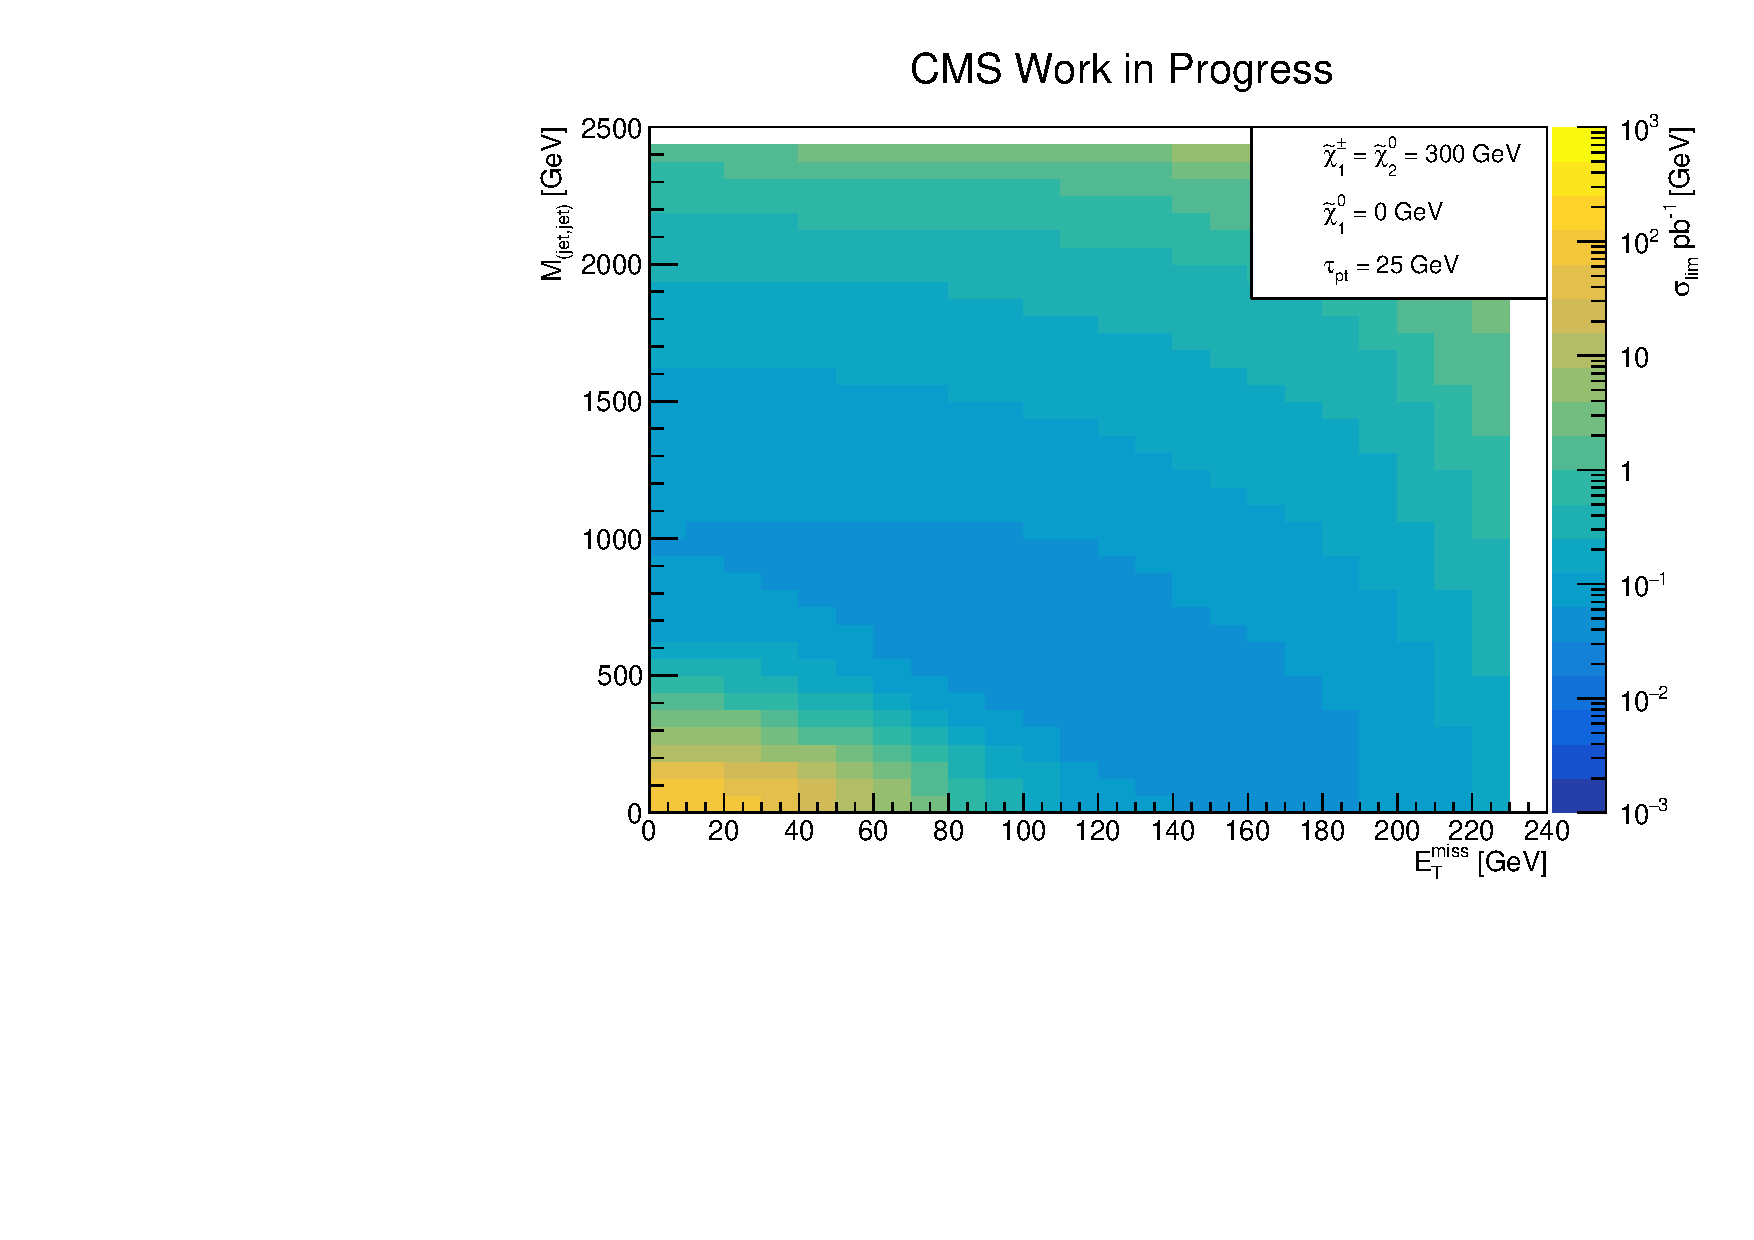
\includegraphics[width=0.45\textwidth]{analysis/pics/JetInvMass_vs_MET_xsec_chi300_lsp000_taupt25.pdf}
		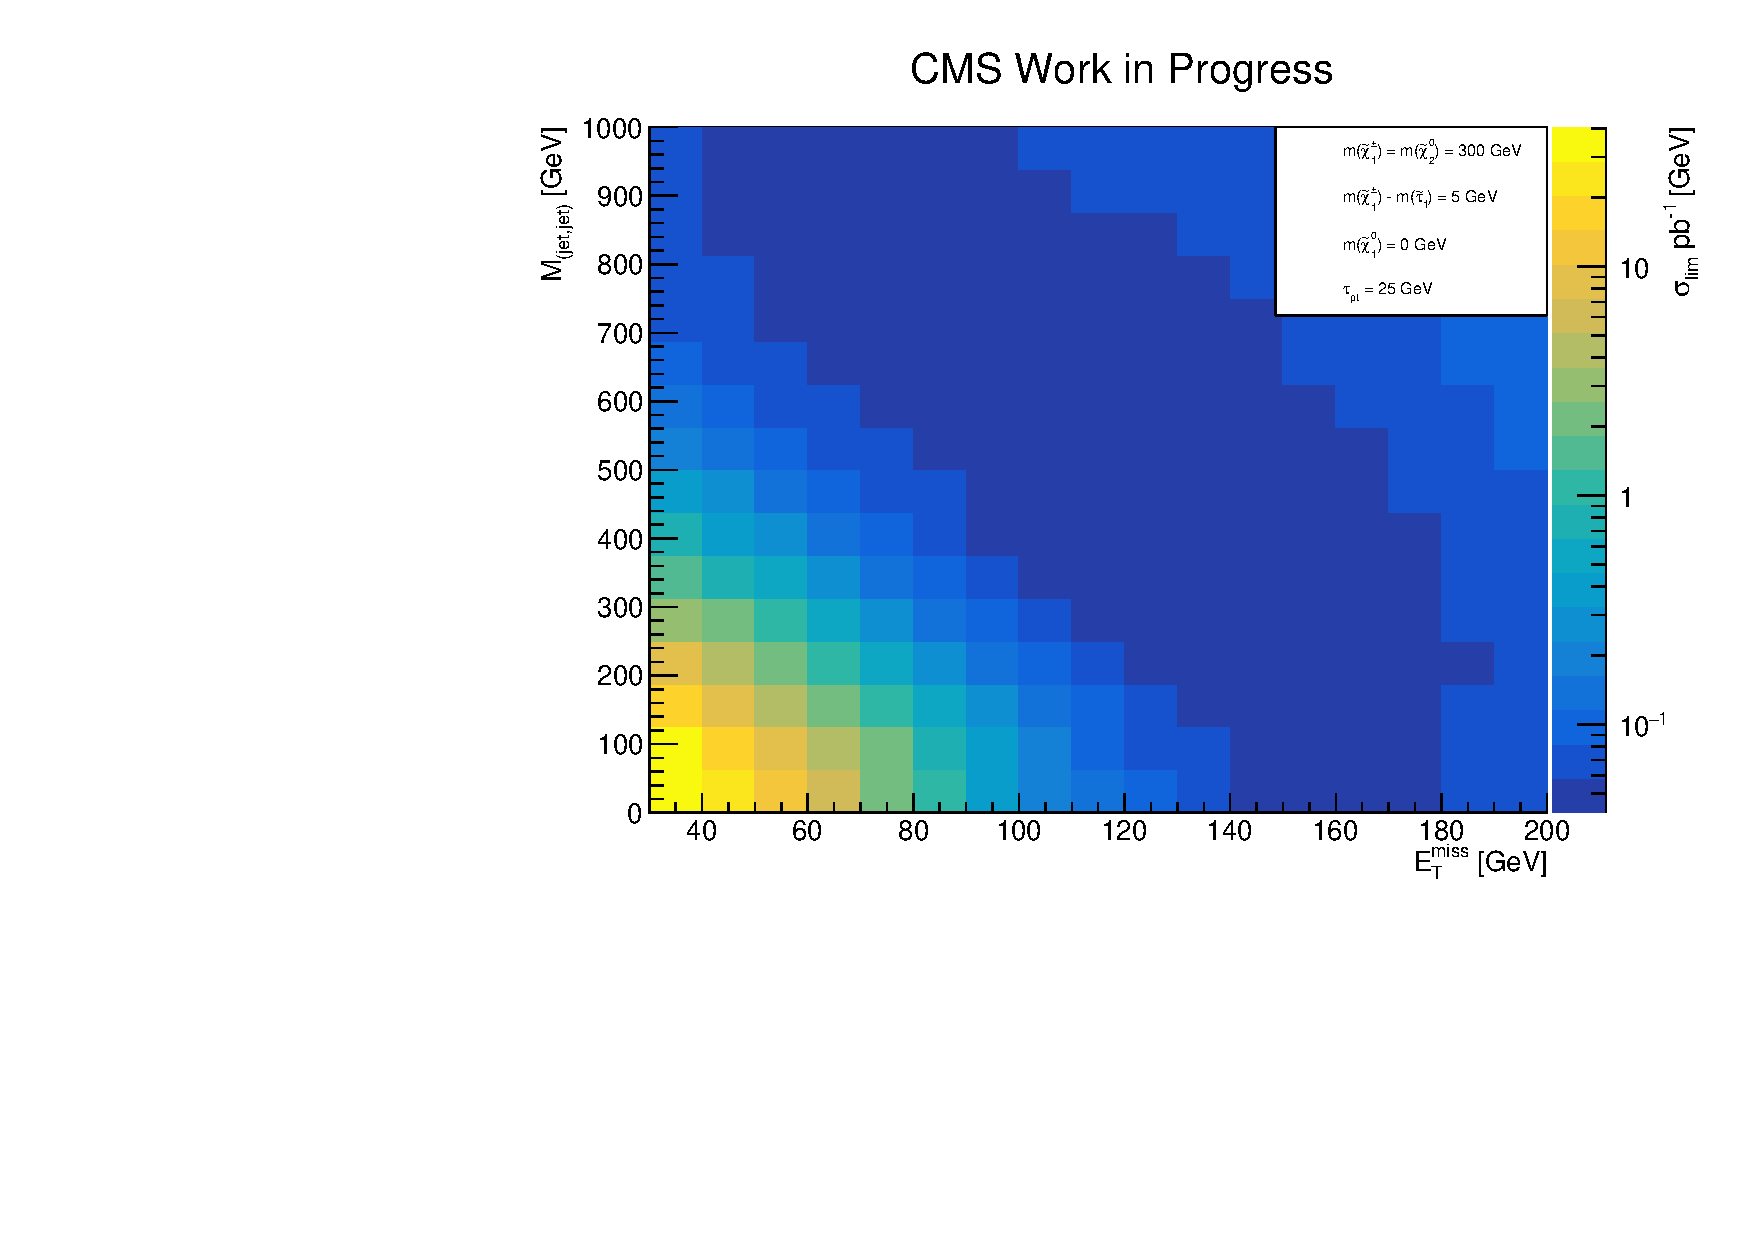
\includegraphics[width=0.45\textwidth]{analysis/pics/JetInvMass_vs_MET_xsec_chi300_lsp000_taupt25_zoom.pdf} 		
	\end{tabular}
	\caption{(Left) Cross section limit as function of $m_{jj}$ and \met for \charginopm = \neutralinotwo = 300 GeV, \neutralinoone = 0 GeV and an offline selection on $\pt(\hadtau) <  25\gev$. (Right) Zooming into the minimum cross section limit area for the same benchmark point.}
	\label{fig::JetInvMass_vs_MET_xsec_chi300_lsp000_taupt25}
\end{figure}

\begin{figure}[tbh!]
	\centering
	\begin{tabular}{cc}
		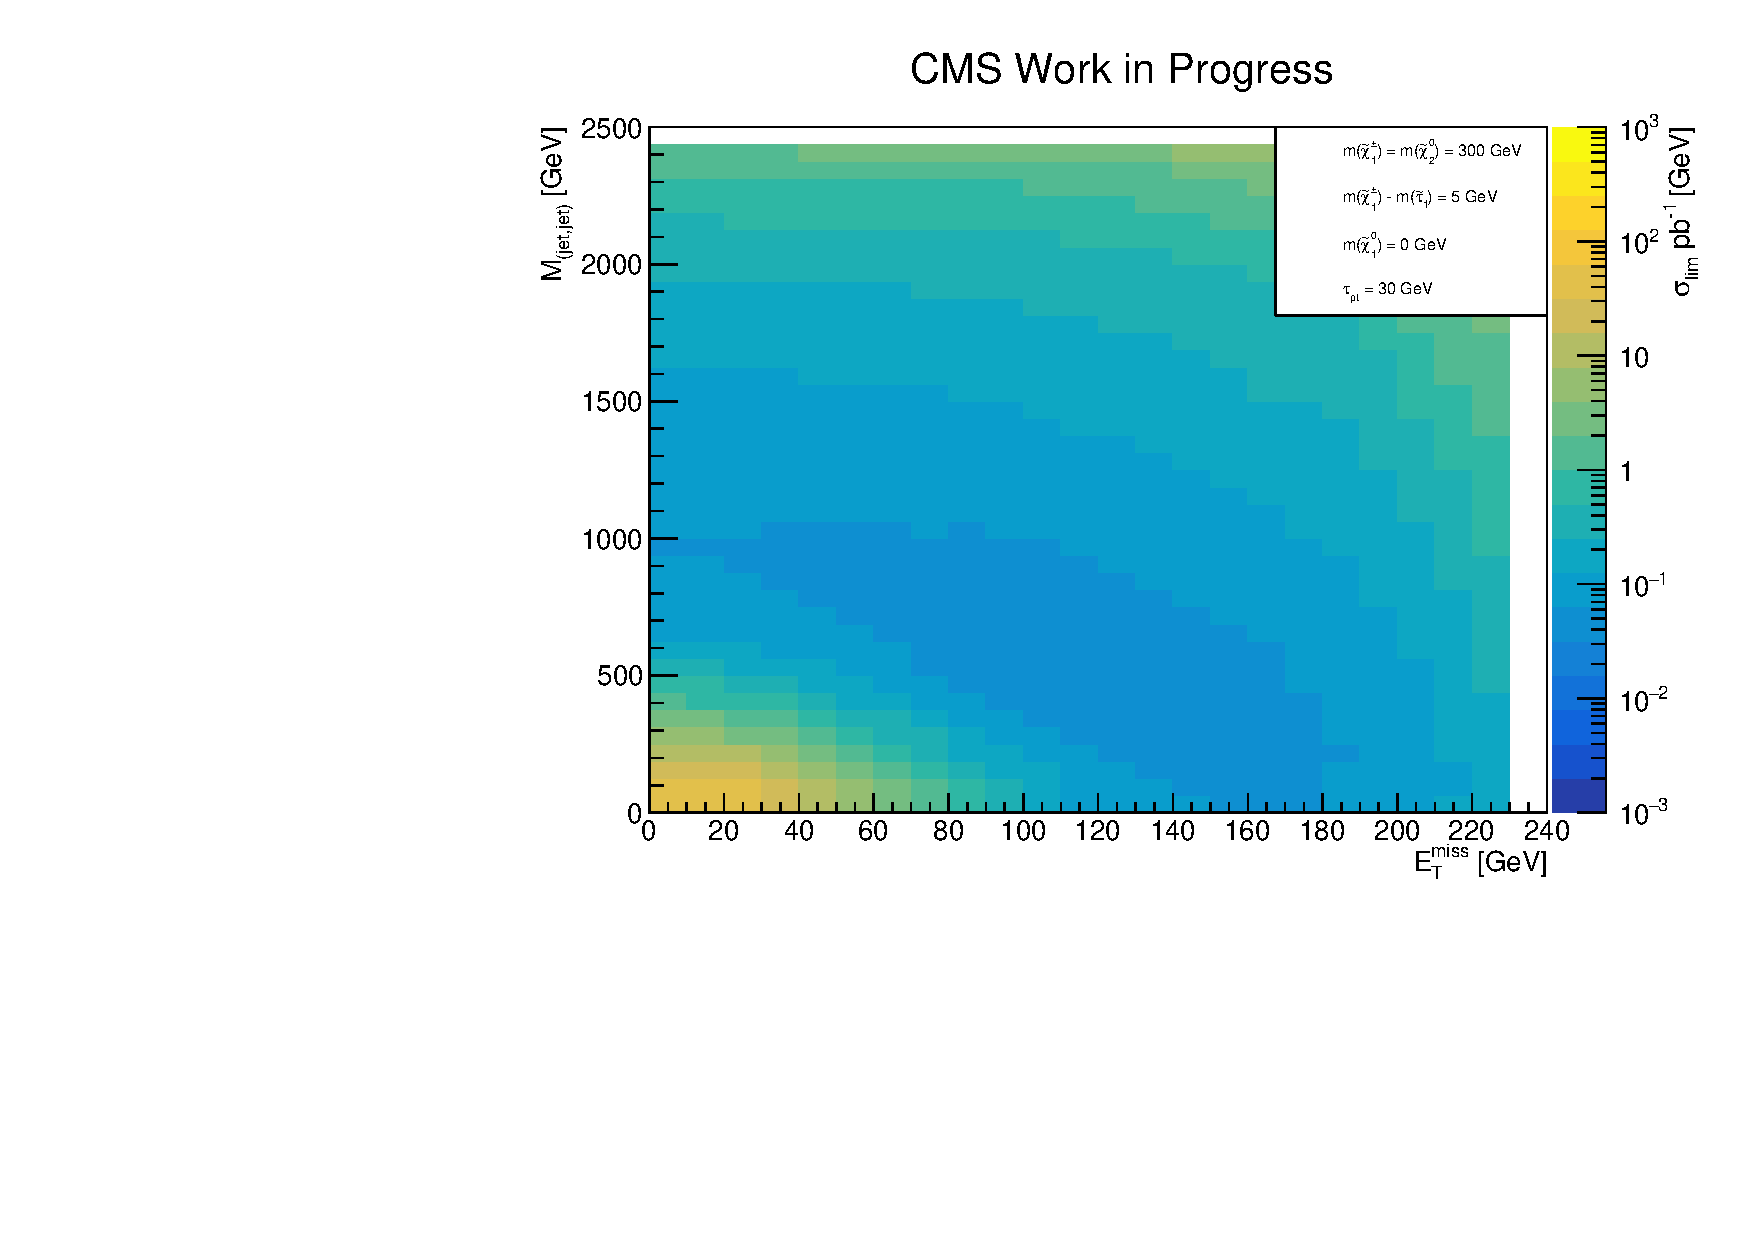
\includegraphics[width=0.45\textwidth]{analysis/pics/JetInvMass_vs_MET_xsec_chi300_lsp000_taupt30.pdf}
		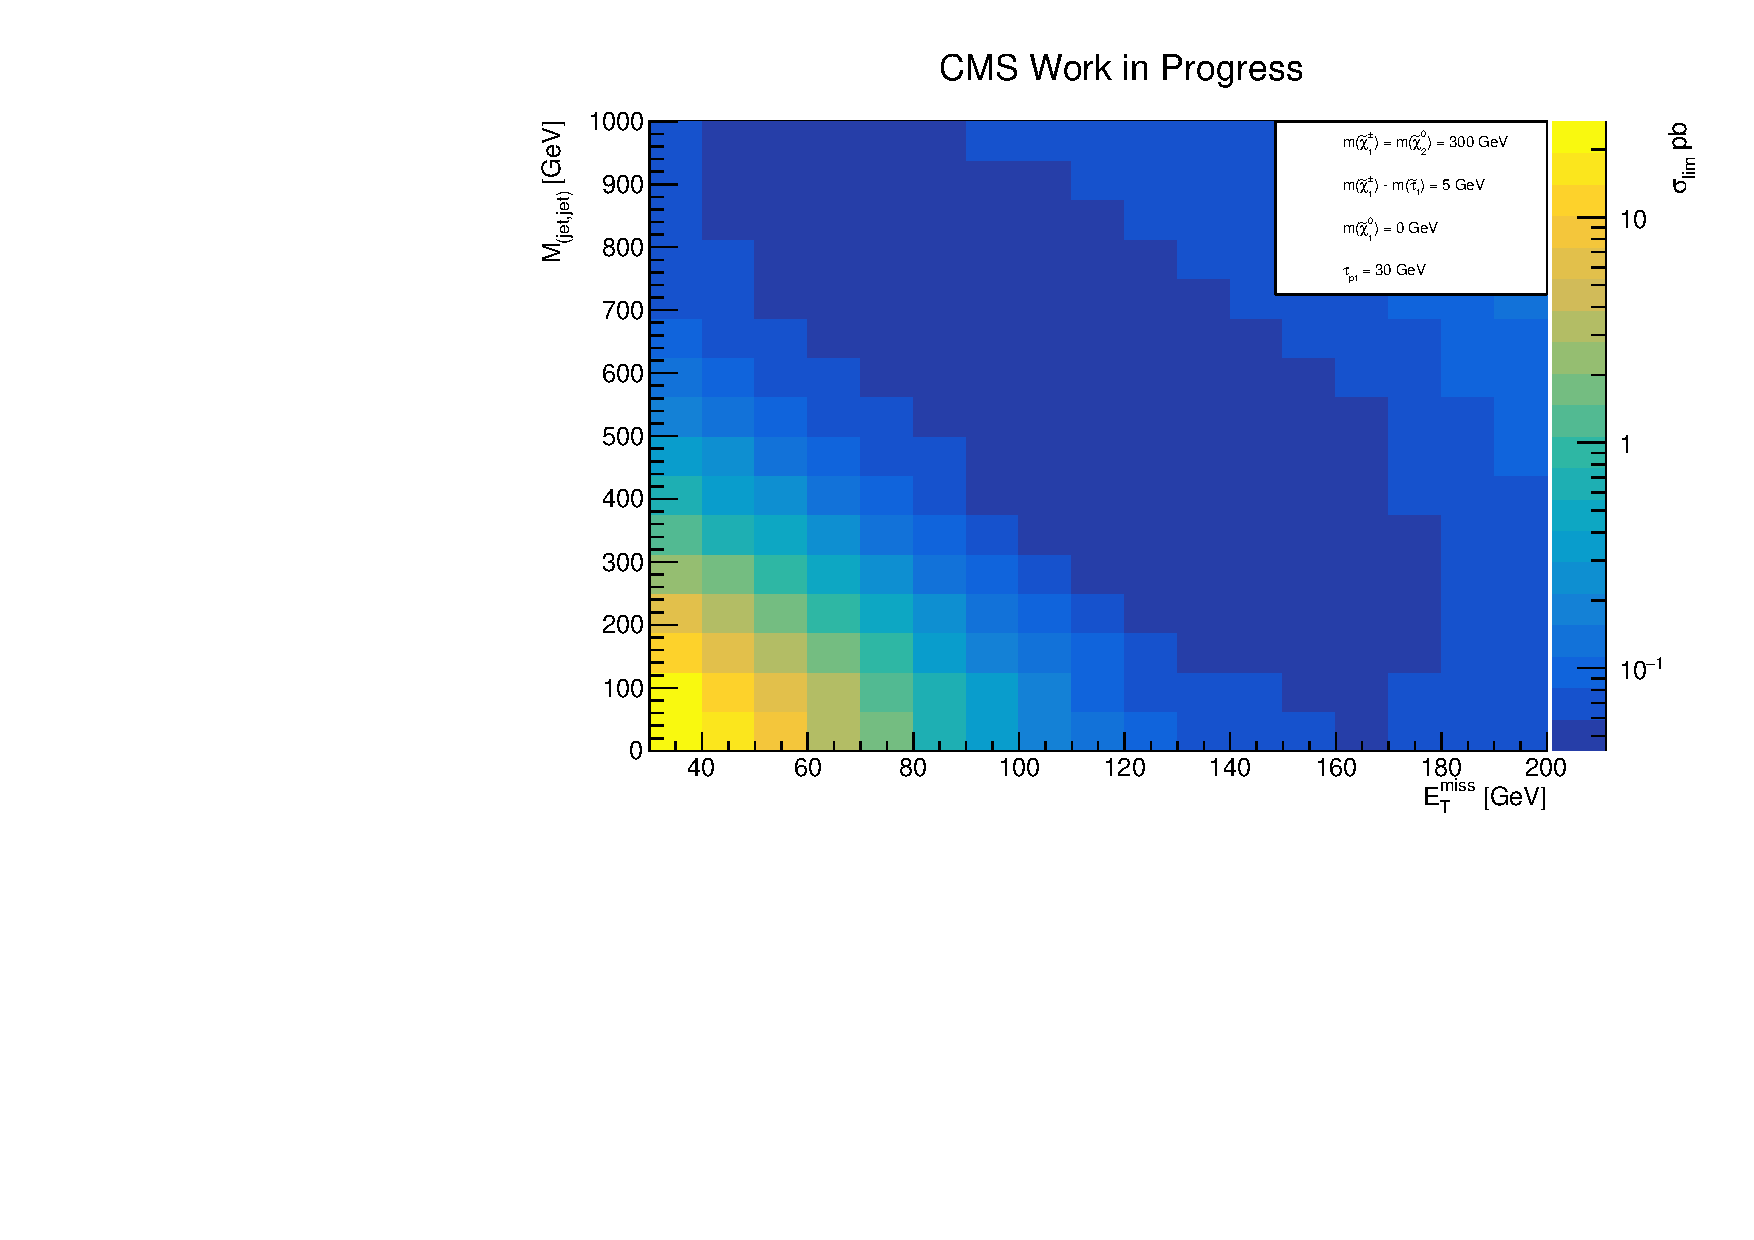
\includegraphics[width=0.45\textwidth]{analysis/pics/JetInvMass_vs_MET_xsec_chi300_lsp000_taupt30_zoom.pdf} 		
	\end{tabular}
	\caption{(Left) Cross section limit as function of $m_{jj}$ and \met for \charginopm = \neutralinotwo = 300 GeV, \neutralinoone = 0 GeV and an offline selection on $\pt(\hadtau) <  30\gev$. (Right) Zooming into the minimum cross section limit area for the same benchmark point.}
	\label{fig::JetInvMass_vs_MET_xsec_chi300_lsp000_taupt30}
\end{figure}

\begin{figure}[tbh!]
	\centering
	\begin{tabular}{cc}
		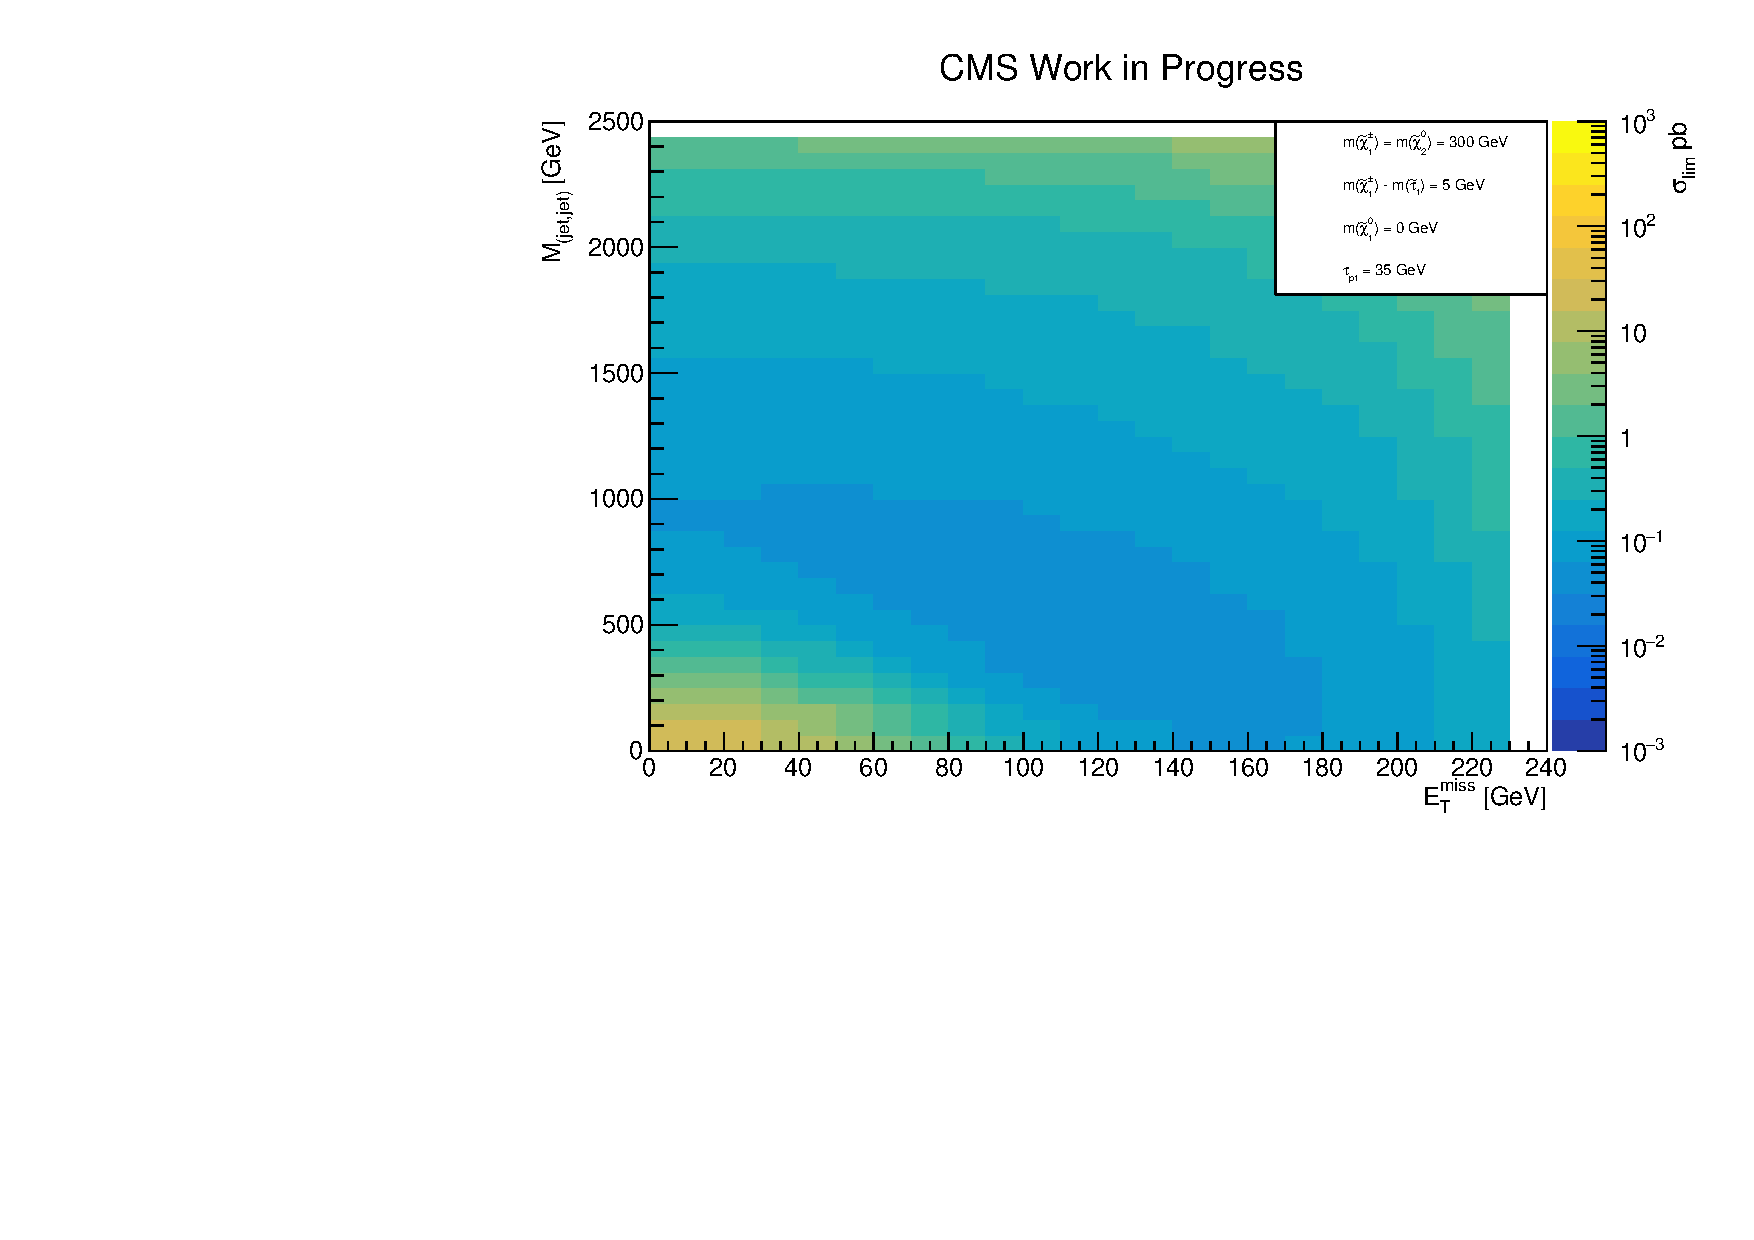
\includegraphics[width=0.45\textwidth]{analysis/pics/JetInvMass_vs_MET_xsec_chi300_lsp000_taupt35.pdf}
		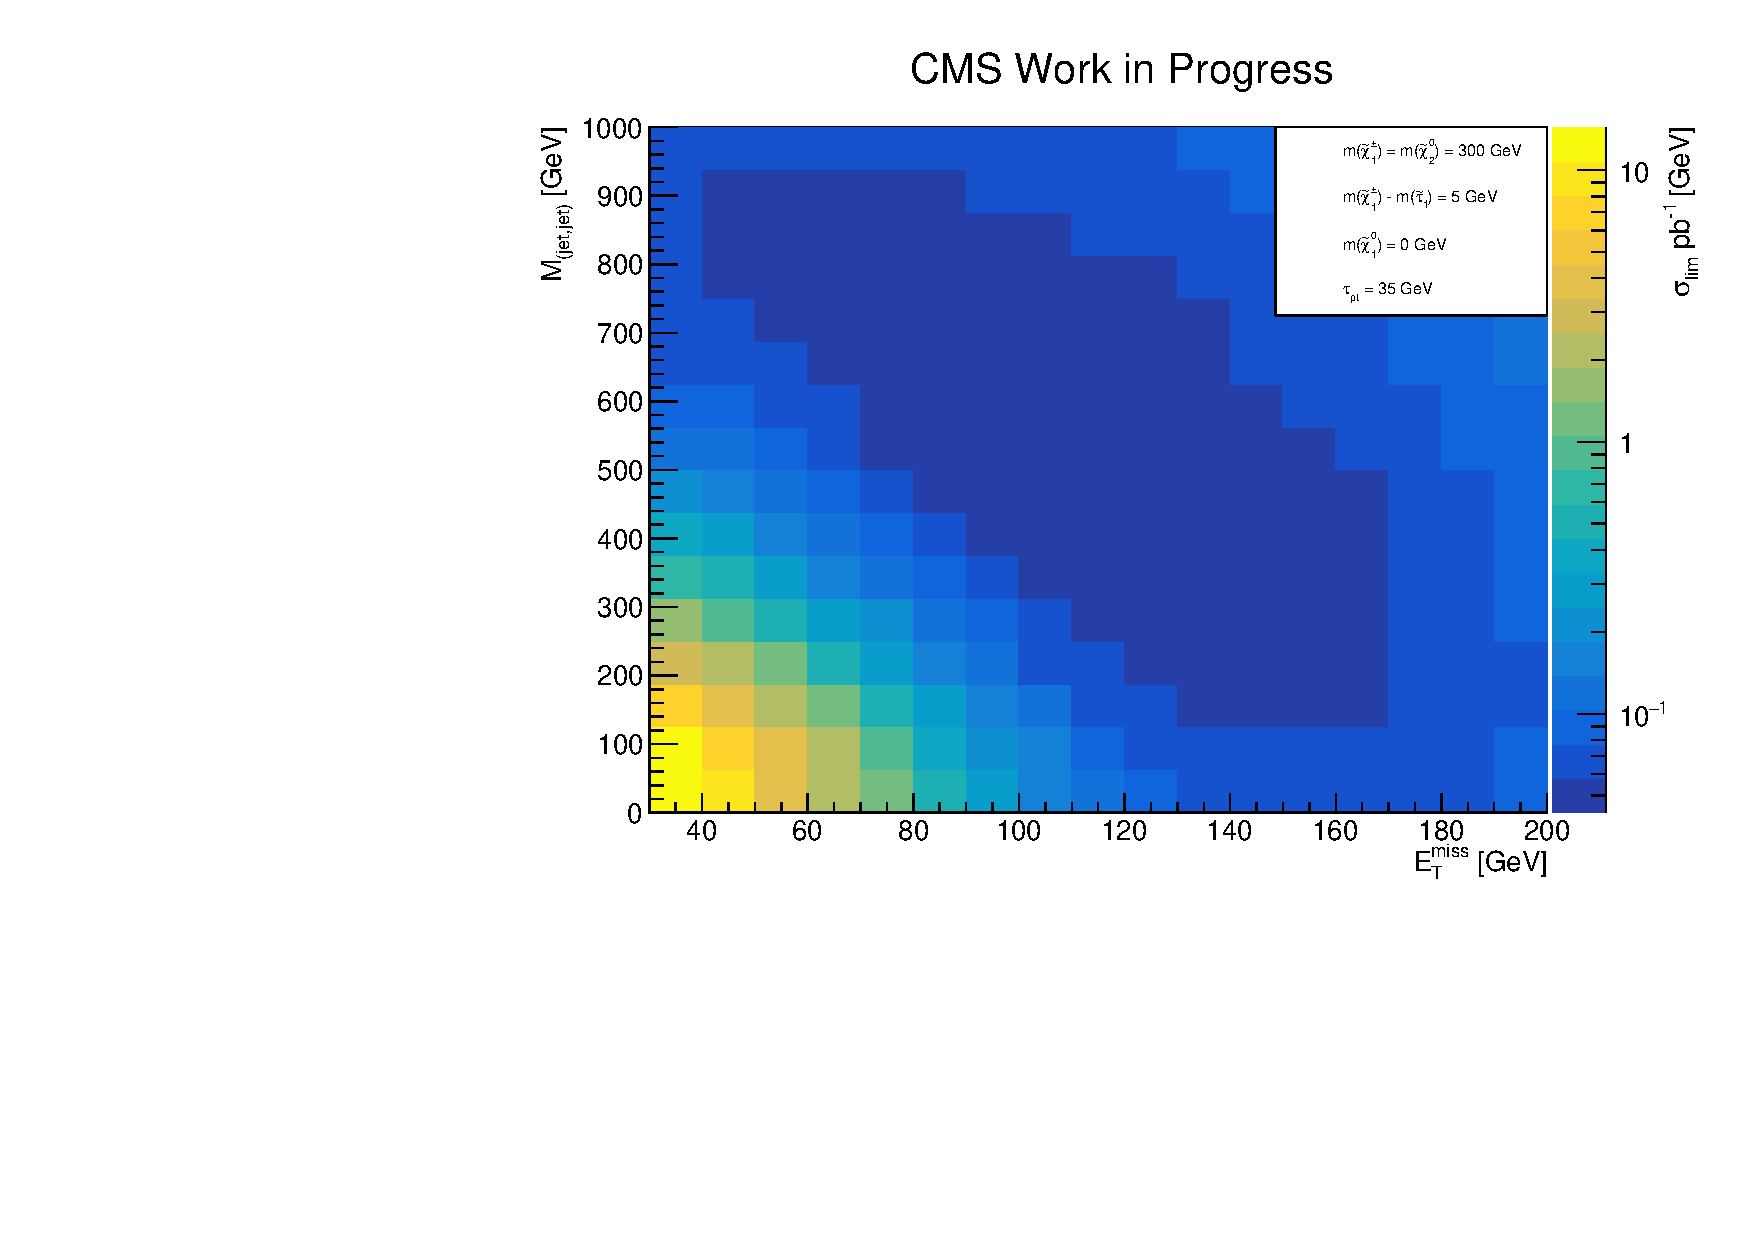
\includegraphics[width=0.45\textwidth]{analysis/pics/JetInvMass_vs_MET_xsec_chi300_lsp000_taupt35_zoom.pdf} 		
	\end{tabular}
	\caption{(Left) Cross section limit as function of $m_{jj}$ and \met for \charginopm = \neutralinotwo = 300 GeV, \neutralinoone = 0 GeV and an offline selection on $\pt(\hadtau) <  35\gev$. (Right) Zooming into the minimum cross section limit area for the same benchmark point.}
	\label{fig::JetInvMass_vs_MET_xsec_chi300_lsp000_taupt35}
\end{figure}

\begin{figure}[tbh!]
	\centering
	\begin{tabular}{cc}
		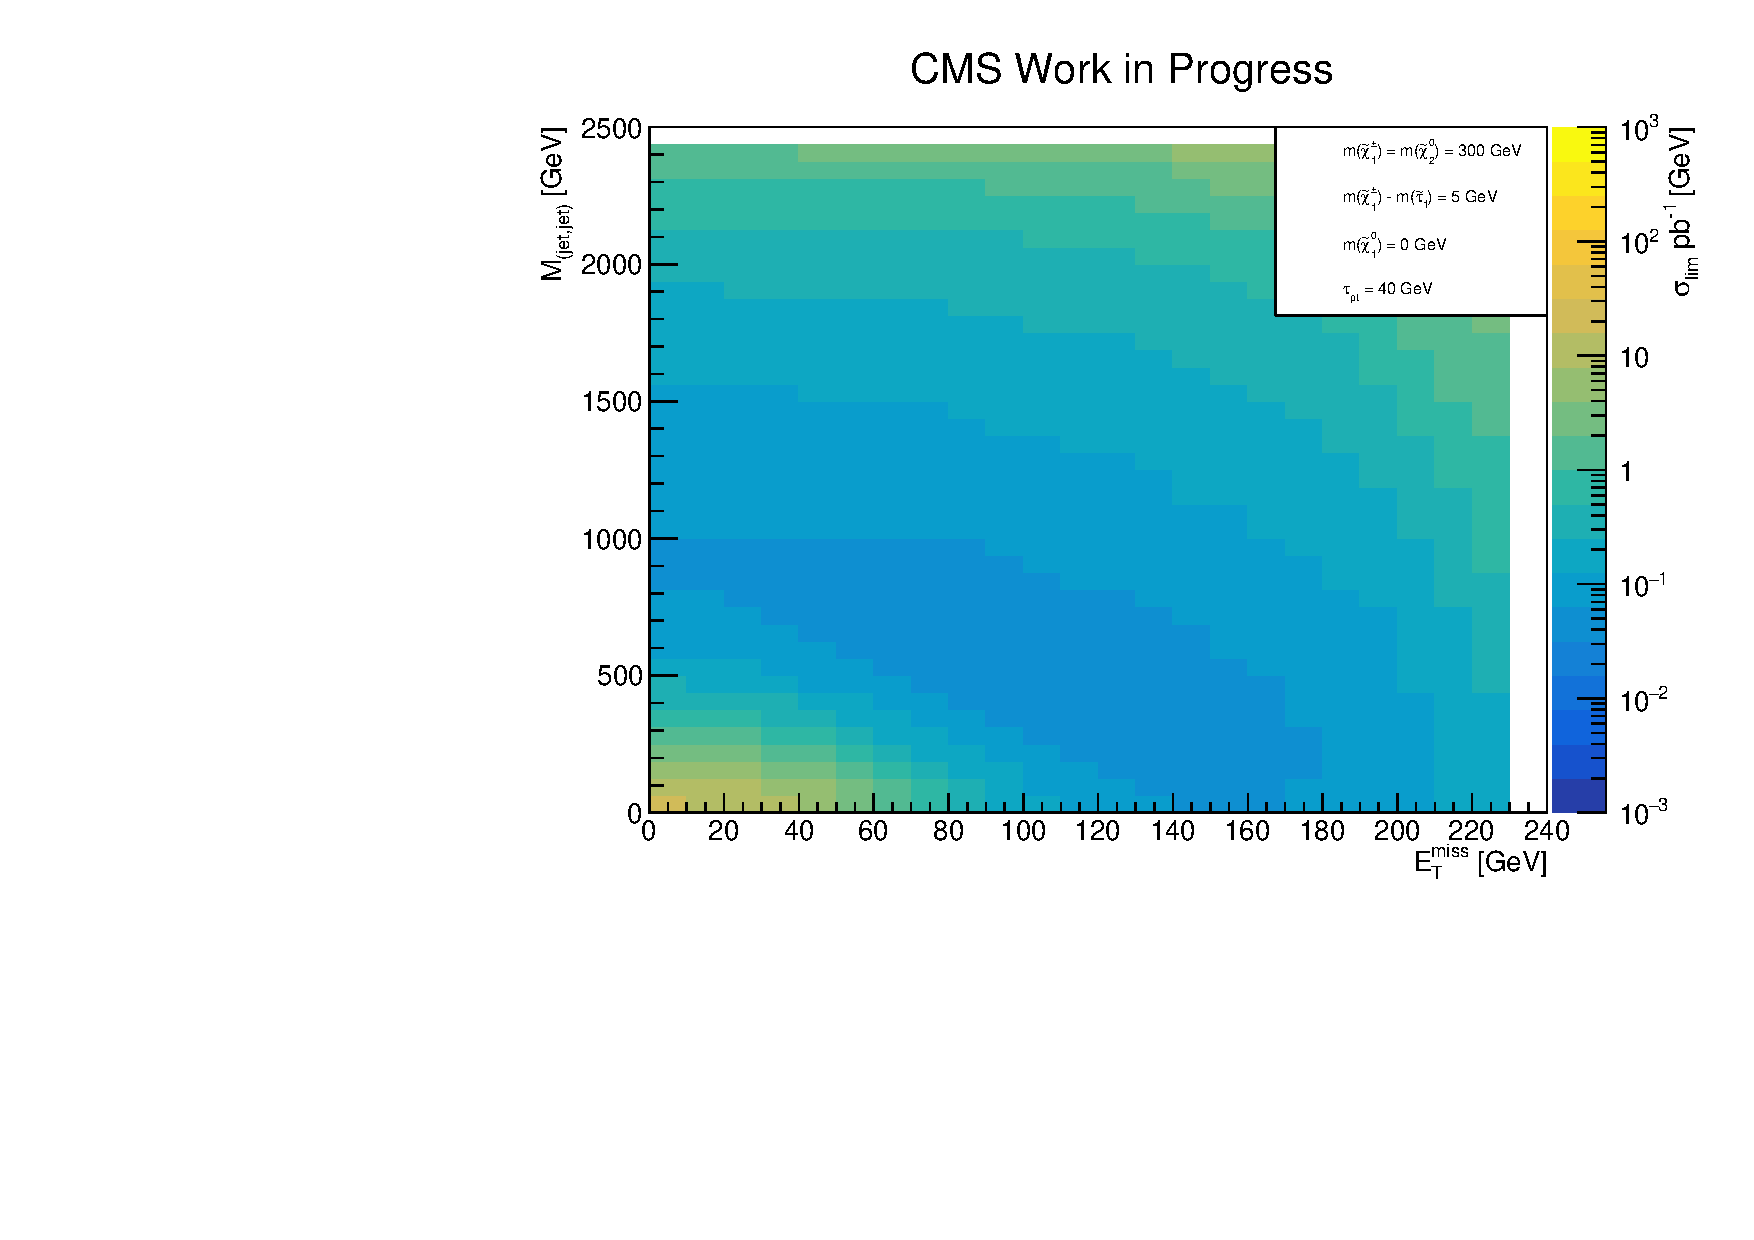
\includegraphics[width=0.45\textwidth]{analysis/pics/JetInvMass_vs_MET_xsec_chi300_lsp000_taupt40.pdf}
		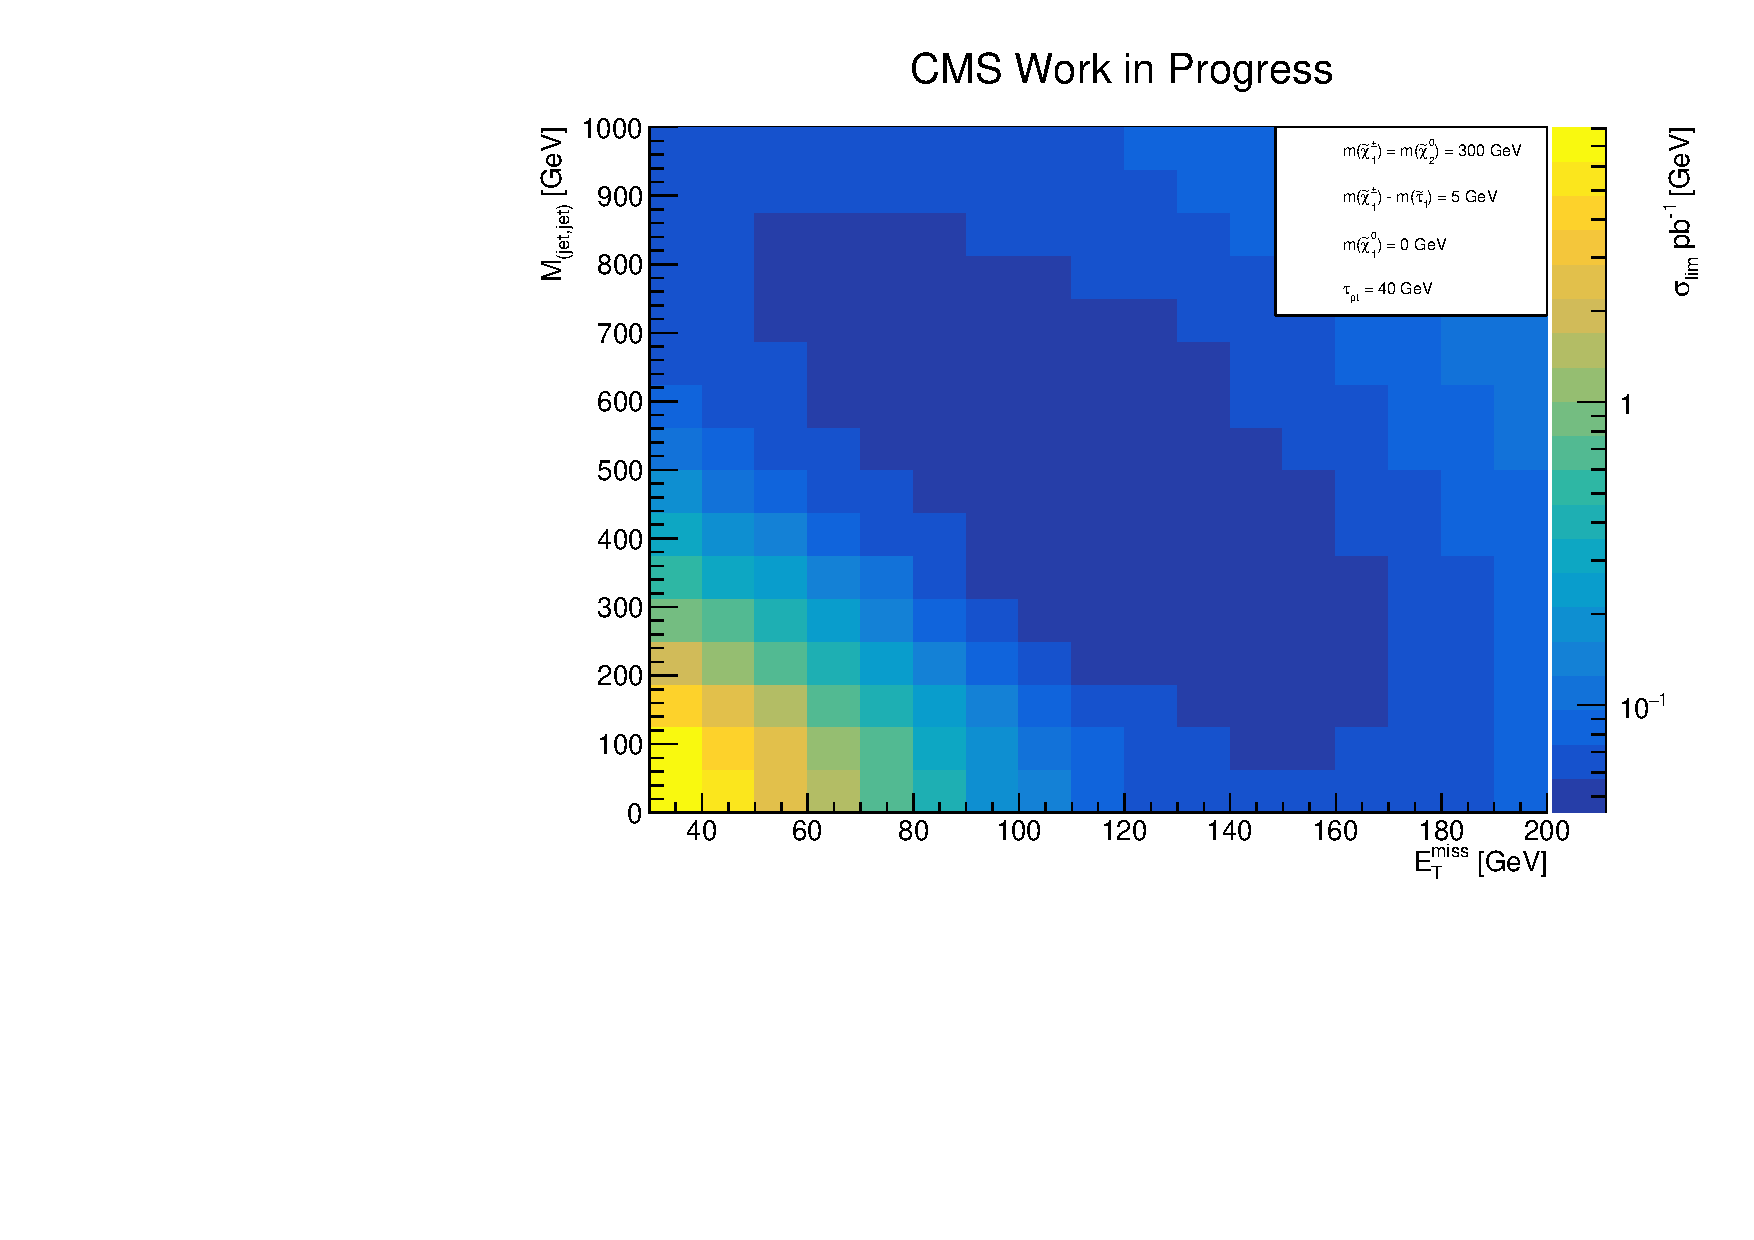
\includegraphics[width=0.45\textwidth]{analysis/pics/JetInvMass_vs_MET_xsec_chi300_lsp000_taupt40_zoom.pdf} 		
	\end{tabular}
	\caption{(Left) Cross section limit as function of $m_{jj}$ and \met for \charginopm = \neutralinotwo = 300 GeV, \neutralinoone = 0 GeV and an offline selection on $\pt(\hadtau) <  40\gev$. (Right) Zooming into the minimum cross section limit area for the same benchmark point.}
	\label{fig::JetInvMass_vs_MET_xsec_chi300_lsp000_taupt40}
\end{figure}

\begin{figure}[tbh!]
	\centering
	\begin{tabular}{cc}
		\includegraphics[width=0.45\textwidth]{analysis/pics/JetInvMass_vs_MET_xsec_chi300_lsp000_taupt45.pdf}
		\includegraphics[width=0.45\textwidth]{analysis/pics/JetInvMass_vs_MET_xsec_chi300_lsp000_taupt45_zoom.pdf} 		
	\end{tabular}
	\caption{(Left) Cross section limit as function of $m_{jj}$ and \met for \charginopm = \neutralinotwo = 300 GeV, \neutralinoone = 0 GeV and an offline selection on $\pt(\hadtau) <  45\gev$. (Right) Zooming into the minimum cross section limit area for the same benchmark point.}
	\label{fig::JetInvMass_vs_MET_xsec_chi300_lsp000_taupt45}
\end{figure}

\FloatBarrier

\subsection*{\charginopm = \neutralinotwo = 100 GeV, \neutralinoone = 50 GeV}

\FloatBarrier

\begin{table}
	\begin{center}
		
		
		\begin{tabular}{| c | c | c | c | }
			\toprule
			\multicolumn{4}{| c | }{m(\charginopm) = m(\neutralinotwo) = 100\gev; m(\neutralinoone) = 50\gev} \\
			\midrule
			$\sigma_{lim}^{min}\pm(stat.)\pm(MC syst.)$ [pb]  & \pt(\hadtau) [GeV] & \mjj [GeV] & \met [GeV] \\
			\midrule
			$0.0334451\pm0.00696054^{+0.00319223}_{-0.00376567}$ & $<$ 20 & $<$ 250  & $<$ 130 \\
			
			$0.039929\pm0.00629768^{+0.00300536}_{-0.00364849}$ & $<$ 25 & $<$ 500  & $<$ 110 \\
			
			$0.0419618\pm0.00915456^{+0.00411594}_{-0.00483792}$ & $<$ 30 & $<$ 375  & $<$ 120 \\
			
			$0.0420015\pm0.00750813^{+0.00350443}_{-0.00420426}$ & $<$ 35 & $<$ 375  & $<$ 120 \\
			
			$0.0419907\pm0.00814932^{+0.00378484}_{-0.0044977}$ & $<$ 40 & $<$ 375  & $<$ 110 \\
			
			$0.0426807\pm0.00688805^{+0.00330145}_{-0.00399578}$ & $<$ 45 & $<$ 375  & $<$ 110 \\
			
			\bottomrule
		\end{tabular}\caption{Cross section limit minimum reached at the given cuts for $m_{jj}$, \met and an increasing \pt(\hadtau) for \charginopm = \neutralinotwo = 100 GeV, \neutralinoone = 50 GeV benchmark point.}
		\label{table::xseclimmin_chi100_lsp050}
	\end{center}
\end{table}

\begin{figure}[tbh!]
	\centering
	\begin{tabular}{cc}
		\includegraphics[width=0.45\textwidth]{analysis/pics/JetInvMass_vs_MET_xsec_chi100_lsp050_taupt20.pdf}
		\includegraphics[width=0.45\textwidth]{analysis/pics/JetInvMass_vs_MET_xsec_chi100_lsp050_taupt20_zoom.pdf} 		
	\end{tabular}
	\caption{(Left) Cross section limit as function of $m_{jj}$ and \met for \charginopm = \neutralinotwo = 100 GeV, \neutralinoone = 50 GeV and an offline selection on $\pt(\hadtau) <  20\gev$. (Right) Zooming into the minimum cross section limit area for the same benchmark point.}
	\label{fig::JetInvMass_vs_MET_xsec_chi100_lsp050_taupt20}
\end{figure}

\begin{figure}[tbh!]
	\centering
	\begin{tabular}{cc}
		\includegraphics[width=0.45\textwidth]{analysis/pics/JetInvMass_vs_MET_xsec_chi100_lsp050_taupt25.pdf}
		\includegraphics[width=0.45\textwidth]{analysis/pics/JetInvMass_vs_MET_xsec_chi100_lsp050_taupt25_zoom.pdf} 		
	\end{tabular}
	\caption{(Left) Cross section limit as function of $m_{jj}$ and \met for \charginopm = \neutralinotwo = 100 GeV, \neutralinoone = 50 GeV and an offline selection on $\pt(\hadtau) <  25\gev$. (Right) Zooming into the minimum cross section limit area for the same benchmark point.}
	\label{fig::JetInvMass_vs_MET_xsec_chi100_lsp050_taupt25}
\end{figure}

\begin{figure}[tbh!]
	\centering
	\begin{tabular}{cc}
		\includegraphics[width=0.45\textwidth]{analysis/pics/JetInvMass_vs_MET_xsec_chi100_lsp050_taupt30.pdf}
		\includegraphics[width=0.45\textwidth]{analysis/pics/JetInvMass_vs_MET_xsec_chi100_lsp050_taupt30_zoom.pdf} 		
	\end{tabular}
	\caption{(Left) Cross section limit as function of $m_{jj}$ and \met for \charginopm = \neutralinotwo = 100 GeV, \neutralinoone = 50 GeV and an offline selection on $\pt(\hadtau) <  30\gev$. (Right) Zooming into the minimum cross section limit area for the same benchmark point.}
	\label{fig::JetInvMass_vs_MET_xsec_chi100_lsp050_taupt30}
\end{figure}

\begin{figure}[tbh!]
	\centering
	\begin{tabular}{cc}
		\includegraphics[width=0.45\textwidth]{analysis/pics/JetInvMass_vs_MET_xsec_chi100_lsp050_taupt35.pdf}
		\includegraphics[width=0.45\textwidth]{analysis/pics/JetInvMass_vs_MET_xsec_chi100_lsp050_taupt35_zoom.pdf} 		
	\end{tabular}
	\caption{(Left) Cross section limit as function of $m_{jj}$ and \met for \charginopm = \neutralinotwo = 100 GeV, \neutralinoone = 50 GeV and an offline selection on $\pt(\hadtau) <  35\gev$. (Right) Zooming into the minimum cross section limit area for the same benchmark point.}
	\label{fig::JetInvMass_vs_MET_xsec_chi100_lsp050_taupt35}
\end{figure}

\begin{figure}[tbh!]
	\centering
	\begin{tabular}{cc}
		\includegraphics[width=0.45\textwidth]{analysis/pics/JetInvMass_vs_MET_xsec_chi100_lsp050_taupt40.pdf}
		\includegraphics[width=0.45\textwidth]{analysis/pics/JetInvMass_vs_MET_xsec_chi100_lsp050_taupt40_zoom.pdf} 		
	\end{tabular}
	\caption{(Left) Cross section limit as function of $m_{jj}$ and \met for \charginopm = \neutralinotwo = 100 GeV, \neutralinoone = 50 GeV and an offline selection on $\pt(\hadtau) <  40\gev$. (Right) Zooming into the minimum cross section limit area for the same benchmark point.}
	\label{fig::JetInvMass_vs_MET_xsec_chi100_lsp050_taupt40}
\end{figure}

\begin{figure}[tbh!]
	\centering
	\begin{tabular}{cc}
		\includegraphics[width=0.45\textwidth]{analysis/pics/JetInvMass_vs_MET_xsec_chi100_lsp050_taupt45.pdf}
		\includegraphics[width=0.45\textwidth]{analysis/pics/JetInvMass_vs_MET_xsec_chi100_lsp050_taupt45_zoom.pdf} 		
	\end{tabular}
	\caption{(Left) Cross section limit as function of $m_{jj}$ and \met for \charginopm = \neutralinotwo = 100 GeV, \neutralinoone = 50 GeV and an offline selection on $\pt(\hadtau) <  45\gev$. (Right) Zooming into the minimum cross section limit area for the same benchmark point.}
	\label{fig::JetInvMass_vs_MET_xsec_chi100_lsp050_taupt45}
\end{figure}

\FloatBarrier

\subsection*{\charginopm = \neutralinotwo = 200 GeV, \neutralinoone = 50 GeV}

\FloatBarrier

\begin{table}
	\begin{center}
		
		
		\begin{tabular}{| c | c | c | c | }
			\toprule
			\multicolumn{4}{| c | }{m(\charginopm) = m(\neutralinotwo) = 200\gev; m(\neutralinoone) = 50\gev} \\
			\midrule
			$\sigma_{lim}^{min}\pm(stat.)\pm(MC syst.)$ [pb]  & \pt(\hadtau) [GeV] & \mjj [GeV] & \met [GeV] \\
			\midrule
			$0.0336268\pm0.00683305^{+0.00314131}_{-0.00371595}$ & $<$ 20 & $<$ 312.5  & $<$ 120 \\
			
			$0.0393934\pm0.0062121^{+0.00296505}_{-0.00359956}$ & $<$ 25 & $<$ 500  & $<$ 110 \\

			$0.0414812\pm0.00668346^{+0.00315393}_{-0.00382458}$ & $<$ 30 & $<$ 437.5  & $<$ 120 \\

			$0.0414812\pm0.00668346^{+0.00315393}_{-0.00382458}$ & $<$ 30 & $<$ 437.5  & $<$ 120 \\

			$0.0427707\pm0.00830816^{+0.00385749}_{-0.00458368}$ & $<$ 40 & $<$ 312.5  & $<$ 120 \\
			
			$0.043694\pm0.00724588^{+0.0034566}_{-0.00417288}$ & $<$ 45 & $<$ 312.5  & $<$ 120 \\
			
			\bottomrule
		\end{tabular}\caption{Cross section limit minimum reached at the given cuts for $m_{jj}$, \met and an increasing \pt(\hadtau) for \charginopm = \neutralinotwo = 200 GeV, \neutralinoone = 50 GeV benchmark point.}
		\label{table::xseclimmin_chi200_lsp050}
	\end{center}
\end{table}

\begin{figure}[tbh!]
	\centering
	\begin{tabular}{cc}
		\includegraphics[width=0.45\textwidth]{analysis/pics/JetInvMass_vs_MET_xsec_chi200_lsp050_taupt20.pdf}
		\includegraphics[width=0.45\textwidth]{analysis/pics/JetInvMass_vs_MET_xsec_chi200_lsp050_taupt20_zoom.pdf} 		
	\end{tabular}
	\caption{(Left) Cross section limit as function of $m_{jj}$ and \met for \charginopm = \neutralinotwo = 200 GeV, \neutralinoone = 50 GeV and an offline selection on $\pt(\hadtau) <  20\gev$. (Right) Zooming into the minimum cross section limit area for the same benchmark point.}
	\label{fig::JetInvMass_vs_MET_xsec_chi200_lsp050_taupt20}
\end{figure}

\begin{figure}[tbh!]
	\centering
	\begin{tabular}{cc}
		\includegraphics[width=0.45\textwidth]{analysis/pics/JetInvMass_vs_MET_xsec_chi200_lsp050_taupt25.pdf}
		\includegraphics[width=0.45\textwidth]{analysis/pics/JetInvMass_vs_MET_xsec_chi200_lsp050_taupt25_zoom.pdf} 		
	\end{tabular}
	\caption{(Left) Cross section limit as function of $m_{jj}$ and \met for \charginopm = \neutralinotwo = 200 GeV, \neutralinoone = 50 GeV and an offline selection on $\pt(\hadtau) <  25\gev$. (Right) Zooming into the minimum cross section limit area for the same benchmark point.}
	\label{fig::JetInvMass_vs_MET_xsec_chi200_lsp050_taupt25}
\end{figure}

\begin{figure}[tbh!]
	\centering
	\begin{tabular}{cc}
		\includegraphics[width=0.45\textwidth]{analysis/pics/JetInvMass_vs_MET_xsec_chi200_lsp050_taupt30.pdf}
		\includegraphics[width=0.45\textwidth]{analysis/pics/JetInvMass_vs_MET_xsec_chi200_lsp050_taupt30_zoom.pdf} 		
	\end{tabular}
	\caption{(Left) Cross section limit as function of $m_{jj}$ and \met for \charginopm = \neutralinotwo = 200 GeV, \neutralinoone = 50 GeV and an offline selection on $\pt(\hadtau) <  30\gev$. (Right) Zooming into the minimum cross section limit area for the same benchmark point.}
	\label{fig::JetInvMass_vs_MET_xsec_chi200_lsp050_taupt30}
\end{figure}

\begin{figure}[tbh!]
	\centering
	\begin{tabular}{cc}
		\includegraphics[width=0.45\textwidth]{analysis/pics/JetInvMass_vs_MET_xsec_chi200_lsp050_taupt35.pdf}
		\includegraphics[width=0.45\textwidth]{analysis/pics/JetInvMass_vs_MET_xsec_chi200_lsp050_taupt35_zoom.pdf} 		
	\end{tabular}
	\caption{(Left) Cross section limit as function of $m_{jj}$ and \met for \charginopm = \neutralinotwo = 200 GeV, \neutralinoone = 50 GeV and an offline selection on $\pt(\hadtau) <  35\gev$. (Right) Zooming into the minimum cross section limit area for the same benchmark point.}
	\label{fig::JetInvMass_vs_MET_xsec_chi200_lsp050_taupt35}
\end{figure}

\begin{figure}[tbh!]
	\centering
	\begin{tabular}{cc}
		\includegraphics[width=0.45\textwidth]{analysis/pics/JetInvMass_vs_MET_xsec_chi200_lsp050_taupt40.pdf}
		\includegraphics[width=0.45\textwidth]{analysis/pics/JetInvMass_vs_MET_xsec_chi200_lsp050_taupt40_zoom.pdf} 		
	\end{tabular}
	\caption{(Left) Cross section limit as function of $m_{jj}$ and \met for \charginopm = \neutralinotwo = 200 GeV, \neutralinoone = 50 GeV and an offline selection on $\pt(\hadtau) <  40\gev$. (Right) Zooming into the minimum cross section limit area for the same benchmark point.}
	\label{fig::JetInvMass_vs_MET_xsec_chi200_lsp050_taupt40}
\end{figure}

\begin{figure}[tbh!]
	\centering
	\begin{tabular}{cc}
		\includegraphics[width=0.45\textwidth]{analysis/pics/JetInvMass_vs_MET_xsec_chi200_lsp050_taupt45.pdf}
		\includegraphics[width=0.45\textwidth]{analysis/pics/JetInvMass_vs_MET_xsec_chi200_lsp050_taupt45_zoom.pdf} 		
	\end{tabular}
	\caption{(Left) Cross section limit as function of $m_{jj}$ and \met for \charginopm = \neutralinotwo = 200 GeV, \neutralinoone = 50 GeV and an offline selection on $\pt(\hadtau) <  45\gev$. (Right) Zooming into the minimum cross section limit area for the same benchmark point.}
	\label{fig::JetInvMass_vs_MET_xsec_chi200_lsp050_taupt45}
\end{figure}

\FloatBarrier

\subsection*{\charginopm = \neutralinotwo = 300 GeV, \neutralinoone = 50 GeV}

\FloatBarrier

\begin{table}
	\begin{center}
		
		
		\begin{tabular}{| c | c | c | c | }
			\toprule
			\multicolumn{4}{| c | }{m(\charginopm) = m(\neutralinotwo) = 300\gev; m(\neutralinoone) = 50\gev} \\
			\midrule
			$\sigma_{lim}^{min}\pm(stat.)\pm(MC syst.)$ [pb]  & \pt(\hadtau) [GeV] & \mjj [GeV] & \met [GeV] \\
			\midrule
			$0.0338743\pm0.00515699^{+0.00249324}_{-0.00303415}$ & $<$ 20 & $<$ 312.5  & $<$ 130 \\
			
			$0.0394788\pm0.00857313^{+0.00387191}_{-0.00455115}$ & $<$ 25 & $<$ 312.5  & $<$ 130 \\
			
			$0.0423392\pm0.00894109^{+0.00406293}_{-0.0047894}$ & $<$ 30 & $<$ 437.5  & $<$ 110 \\
			
			$0.0419848\pm0.00719733^{+0.00341055}_{-0.00410465}$ & $<$ 35 & $<$ 437.5  & $<$ 110 \\
			
			$0.0426056\pm0.00606123^{+0.00297067}_{-0.00363573}$ & $<$ 40 & $<$ 437.5  & $<$ 110 \\
			
			$0.043815\pm0.00706105^{+0.00338919}_{-0.00410197}$ & $<$ 45 & $<$ 375  & $<$ 110 \\
			\bottomrule
		\end{tabular}\caption{Cross section limit minimum reached at the given cuts for $m_{jj}$, \met and an increasing \pt(\hadtau) for \charginopm = \neutralinotwo = 300 GeV, \neutralinoone = 50 GeV benchmark point.}
		\label{table::xseclimmin_chi300_lsp050}
	\end{center}
\end{table}

\begin{figure}[tbh!]
	\centering
	\begin{tabular}{cc}
		\includegraphics[width=0.45\textwidth]{analysis/pics/JetInvMass_vs_MET_xsec_chi300_lsp050_taupt20.pdf}
		\includegraphics[width=0.45\textwidth]{analysis/pics/JetInvMass_vs_MET_xsec_chi300_lsp050_taupt20_zoom.pdf} 		
	\end{tabular}
	\caption{(Left) Cross section limit as function of $m_{jj}$ and \met for \charginopm = \neutralinotwo = 300 GeV, \neutralinoone = 50 GeV and an offline selection on $\pt(\hadtau) <  20\gev$. (Right) Zooming into the minimum cross section limit area for the same benchmark point.}
	\label{fig::JetInvMass_vs_MET_xsec_chi300_lsp050_taupt20}
\end{figure}

\begin{figure}[tbh!]
	\centering
	\begin{tabular}{cc}
		\includegraphics[width=0.45\textwidth]{analysis/pics/JetInvMass_vs_MET_xsec_chi300_lsp050_taupt25.pdf}
		\includegraphics[width=0.45\textwidth]{analysis/pics/JetInvMass_vs_MET_xsec_chi300_lsp050_taupt25_zoom.pdf} 		
	\end{tabular}
	\caption{(Left) Cross section limit as function of $m_{jj}$ and \met for \charginopm = \neutralinotwo = 300 GeV, \neutralinoone = 50 GeV and an offline selection on $\pt(\hadtau) <  25\gev$. (Right) Zooming into the minimum cross section limit area for the same benchmark point.}
	\label{fig::JetInvMass_vs_MET_xsec_chi300_lsp050_taupt25}
\end{figure}

\begin{figure}[tbh!]
	\centering
	\begin{tabular}{cc}
		\includegraphics[width=0.45\textwidth]{analysis/pics/JetInvMass_vs_MET_xsec_chi300_lsp050_taupt30.pdf}
		\includegraphics[width=0.45\textwidth]{analysis/pics/JetInvMass_vs_MET_xsec_chi300_lsp050_taupt30_zoom.pdf} 		
	\end{tabular}
	\caption{(Left) Cross section limit as function of $m_{jj}$ and \met for \charginopm = \neutralinotwo = 300 GeV, \neutralinoone = 50 GeV and an offline selection on $\pt(\hadtau) <  30\gev$. (Right) Zooming into the minimum cross section limit area for the same benchmark point.}
	\label{fig::JetInvMass_vs_MET_xsec_chi300_lsp050_taupt30}
\end{figure}

\begin{figure}[tbh!]
	\centering
	\begin{tabular}{cc}
		\includegraphics[width=0.45\textwidth]{analysis/pics/JetInvMass_vs_MET_xsec_chi300_lsp050_taupt35.pdf}
		\includegraphics[width=0.45\textwidth]{analysis/pics/JetInvMass_vs_MET_xsec_chi300_lsp050_taupt35_zoom.pdf} 		
	\end{tabular}
	\caption{(Left) Cross section limit as function of $m_{jj}$ and \met for \charginopm = \neutralinotwo = 300 GeV, \neutralinoone = 50 GeV and an offline selection on $\pt(\hadtau) <  35\gev$. (Right) Zooming into the minimum cross section limit area for the same benchmark point.}
	\label{fig::JetInvMass_vs_MET_xsec_chi300_lsp050_taupt35}
\end{figure}

\begin{figure}[tbh!]
	\centering
	\begin{tabular}{cc}
		\includegraphics[width=0.45\textwidth]{analysis/pics/JetInvMass_vs_MET_xsec_chi300_lsp050_taupt40.pdf}
		\includegraphics[width=0.45\textwidth]{analysis/pics/JetInvMass_vs_MET_xsec_chi300_lsp050_taupt40_zoom.pdf} 		
	\end{tabular}
	\caption{(Left) Cross section limit as function of $m_{jj}$ and \met for \charginopm = \neutralinotwo = 300 GeV, \neutralinoone = 50 GeV and an offline selection on $\pt(\hadtau) <  40\gev$. (Right) Zooming into the minimum cross section limit area for the same benchmark point.}
	\label{fig::JetInvMass_vs_MET_xsec_chi300_lsp050_taupt40}
\end{figure}

\begin{figure}[tbh!]
	\centering
	\begin{tabular}{cc}
		\includegraphics[width=0.45\textwidth]{analysis/pics/JetInvMass_vs_MET_xsec_chi300_lsp050_taupt45.pdf}
		\includegraphics[width=0.45\textwidth]{analysis/pics/JetInvMass_vs_MET_xsec_chi300_lsp050_taupt45_zoom.pdf} 		
	\end{tabular}
	\caption{(Left) Cross section limit as function of $m_{jj}$ and \met for \charginopm = \neutralinotwo = 300 GeV, \neutralinoone = 50 GeV and an offline selection on $\pt(\hadtau) <  45\gev$. (Right) Zooming into the minimum cross section limit area for the same benchmark point.}
	\label{fig::JetInvMass_vs_MET_xsec_chi300_lsp050_taupt45}
\end{figure}

\FloatBarrier

